\documentclass[aspectratio=169,usenames,dvipsnames]{beamer}
%%%CHOOSE ASPECT RATIO ABOVE%%% ... Other possible values are: 1610, 149, 54, 43 and 32

% the Lund University theme
\usetheme{LundUniversity}

% this tells LaTeX how the latex file is encoded
\usepackage[utf8]{inputenc}
\usepackage[british]{babel}

% align the text
\usepackage{ragged2e}

% colors
\usepackage{xcolor}

% to draw feynman diagrams
\usepackage{axodraw2}

% list in line
\usepackage{paralist}

% Dirac notation
\usepackage{physics}

\usepackage{mathtools}

%\usepackage{cancel}
\definecolor{redcancel}{RGB}{255,127,0}
\usepackage[makeroom]{cancel}
\renewcommand{\CancelColor}{\color{redcancel}}

%For use the minipage environment (figures side-by-side)
\usepackage{caption}
\usepackage{subcaption}

% add note to the table
\usepackage{threeparttable}

\usepackage{array}
% add space between rows for the table
\renewcommand{\arraystretch}{1.2}
% make array for the table
\newcolumntype{C}{>{$}c<{$}}
\newcolumntype{L}{>{$}l<{$}}

% this defines the \includegraphics command used for including figures
\usepackage{graphicx}
% Manipulate the placement of figure and tables.
\usepackage{float}

% the amsmath package has a lot of useful stuff for equations,
% especially for ligning up multiple equations
\usepackage{amsmath}
\usepackage{latexsym}
% count equation inside starred align
\newcommand\numberthis{\addtocounter{equation}{1}\tag{\theequation}}

% Fancy verbatim
\usepackage{fancyvrb}

\usepackage[many]{tcolorbox}
\usepackage{empheq}
\usetikzlibrary{shadows}

%\begin{empheq}[box=\tcbhighmath]{align}
%\end{empheq}
%\begin{empheq}[box=\fbox]{align}
%\end{empheq}

\tcbset{
  highlight math style={
    enhanced,
%    colframe=red!60!black,
    colframe=LUCopper,
%    colback=yellow!50,
    arc=4pt,
    boxrule=1pt,
    drop fuzzy shadow
  }
}

% For hyper references that can be browsable
\usepackage{hyperref}
\hypersetup{
    colorlinks=true,
    linkcolor=blue,
    filecolor=magenta,      
    urlcolor=cyan,
}

\newcommand{\tabitem}{%
  \usebeamertemplate{itemize item}\hspace*{\labelsep}}  
\newcommand{\marrow}[5]{%
    \fmfcmd{style_def marrow#1
    expr p = drawarrow subpath (1/4, 3/4) of p shifted 6 #2 withpen pencircle scaled 0.4;
    label.#3(btex #4 etex, point 0.5 of p shifted 6 #2);
    enddef;}
    \fmf{marrow#1,tension=0}{#5}}

%\boldmath
  
\setbeamercovered{transparent}

\setbeamercolor{alerted text}{fg=black}

%%%%%%%%%%%%%%%%%%%%%%%%%%%%%%%%%%%%%%%%%%%%%%%%%%%%%%%%%%%%%%%%%%%%%%%%
\title[Master Thesis Presentation]{\large{SIMPLIFYING QUANTUM GRAVITY CALCULATIONS}}
\titlecolor{LUGreen} % Choose between LUPink, LULBlue, LUIvory, LUGreen
\titleimage{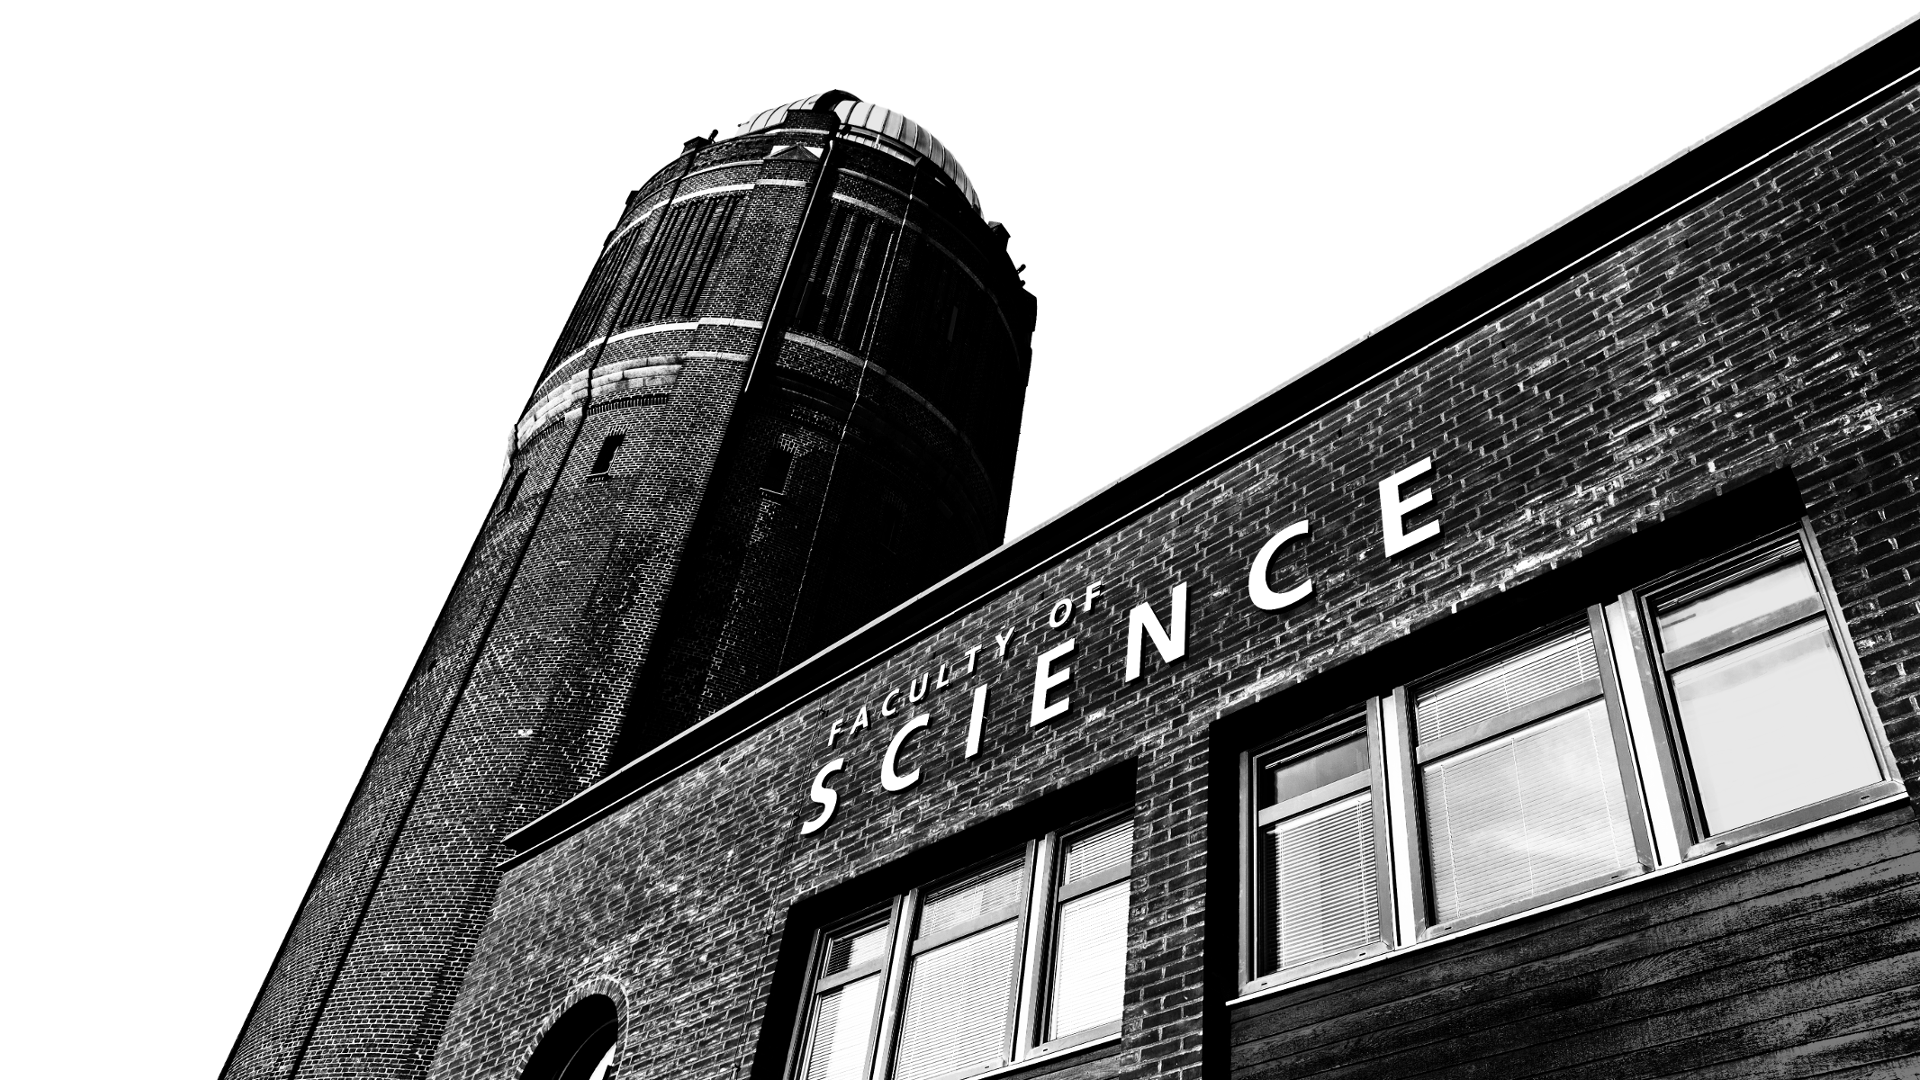
\includegraphics[scale=.5]{images/astro.png}}
%\titleimage{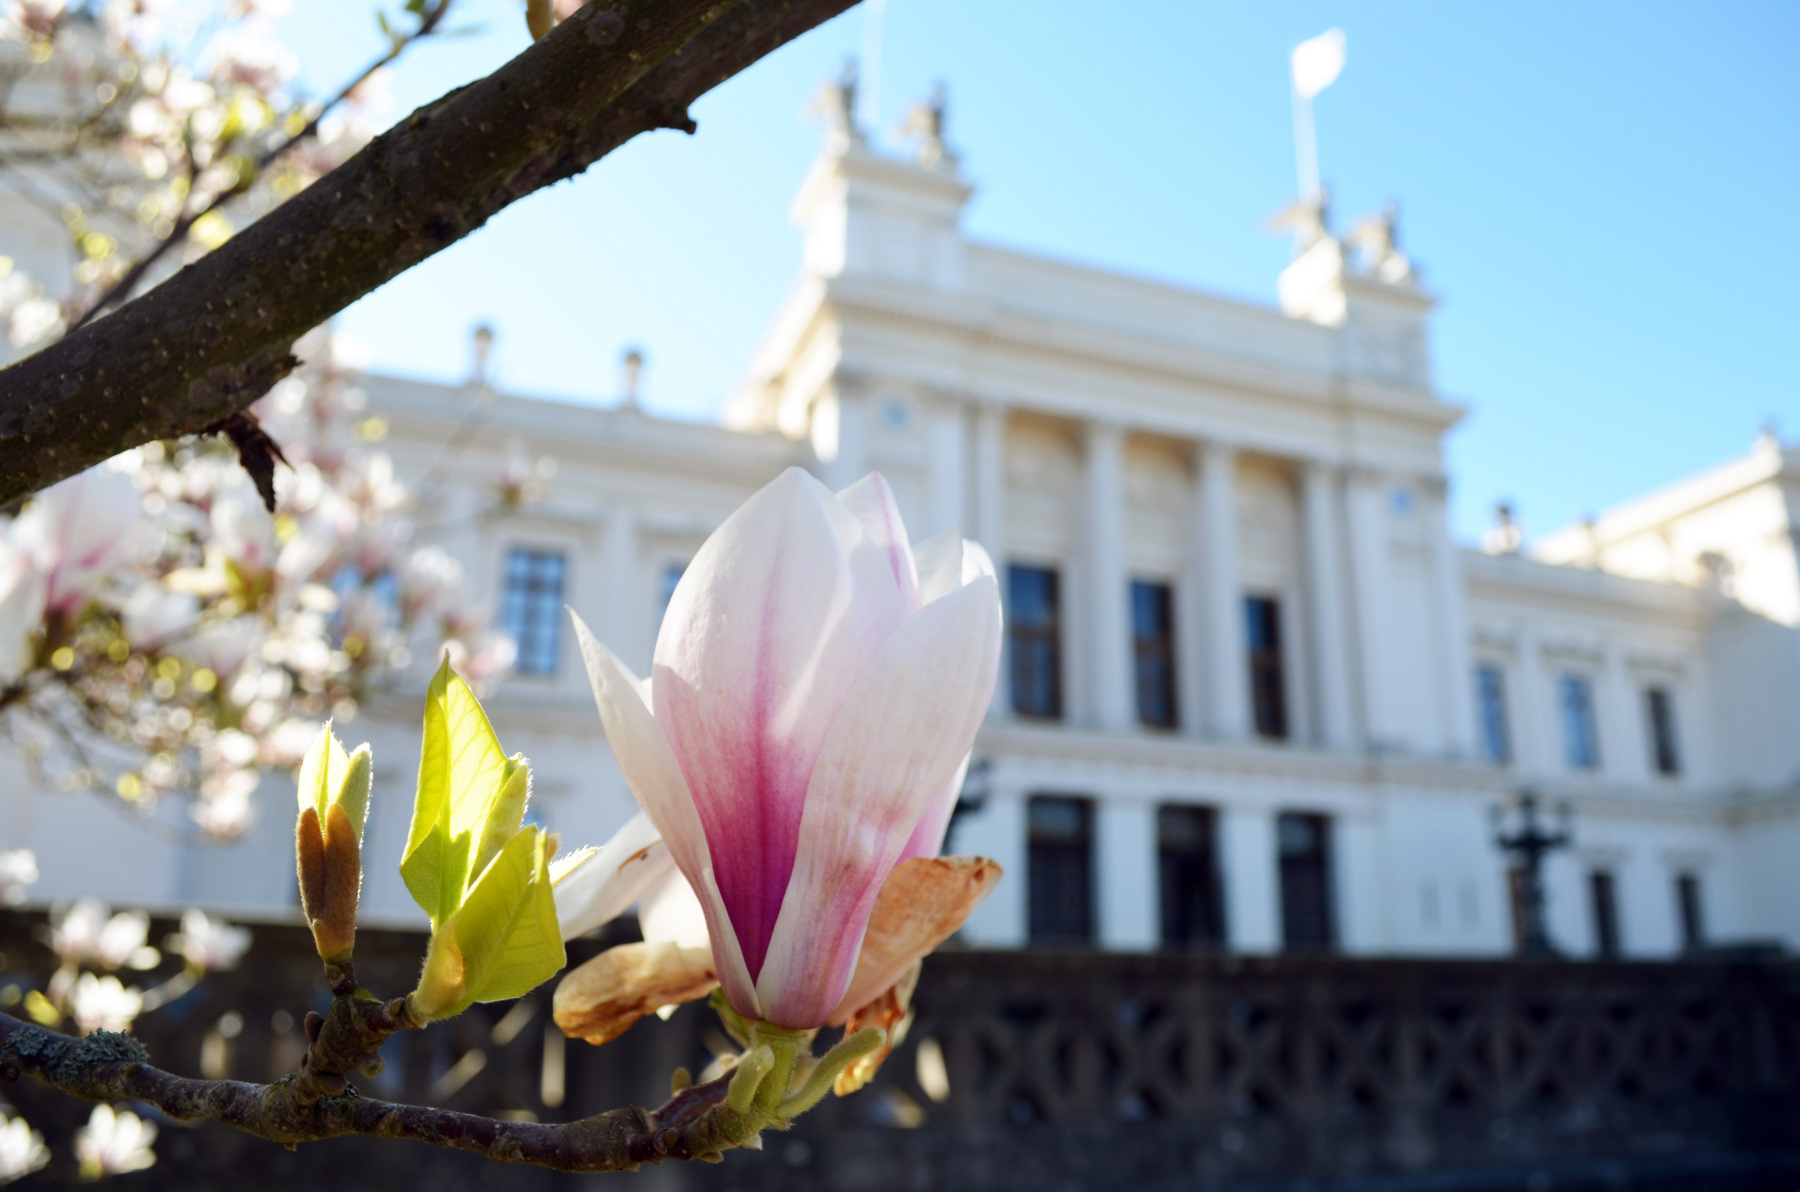
\includegraphics[scale=.6]{images/lumainb.jpg}}
\author{Safi Rafie-Zinedine}
\subtitle{\qquad\, \lowercase{\uppercase{S}afi \uppercase{R}afie-\uppercase{Z}inedine \;\qquad --- \;\qquad \uppercase{S}upervisor: \uppercase{P}rof. \uppercase{J}ohan \uppercase{B}ijnens}}
\date{\today}
\institute{Lund University\\Department of Portals}

\begin{document}
\titleframe

%%%%%%%%%%%%%%%%%%%%%%%%%%%%%%%%%%%%%%%%%%%%%%%%%%%%%%%%%%%%%%%%%%%%%%%%%%%%%%%%%%%%%%
\begin{frame}{Overview} \bf
  \begin{center}
    \begin{minipage}{0.42\textwidth}
      \begin{itemize}
        \item[$\bullet$]      Introduction    \vspace{5.0pt}  \\
        \item[$\bullet$]      Deriving Lagrangian  \\ \vspace{5.0pt} 
        \item[$\bullet$]      Manipulating Lagrangian  \\ \vspace{5.0pt}
        \item[$\bullet$]      Loop Integral  \\ \vspace{5.0pt}
        \item[$\bullet$]      Our Strategies \\ \vspace{5.0pt}
        \item[$\bullet$]      Our Results \\ \vspace{5.0pt}
        \item[$\bullet$]      Scattering at Tree Level \\ \vspace{5.0pt}
        \item[$\bullet$]      Scattering at One-loop Level \\ \vspace{5.0pt}
        \item[$\bullet$]      Conclusions \\ \vspace{40.0pt}
      \end{itemize}
    \end{minipage}
    \vfill
  \end{center}

\vspace*{100mm}
\end{frame}

%%%%%%%%%%%%%%%%%%%%%%%%%%%%%%%%%%%%%%%%%%%%%%%%%%%%%%%%%%%%%%%%%%%%%%%%%%%%%%%%%%%%%%
\section{\bf Introduction}

\begin{frame}{What are the main reasons behind this thesis?}
  \begin{itemize}
  \item[$\bullet$]  The Feynman rules are very complicated although the resulting amplitudes are often simple.
    \vspace{8mm}
  \item[$\bullet$]
    A better understanding of the math in this theory when fewer terms actually contribute.
    \vspace{8mm}
  \item[$\bullet$]  Reducing the running time in FORM program.
    \vspace{8mm}
  \item[$\bullet$]  Following the belief that nature should be described in a beautiful and simple mathematical way.
    \vspace{8mm}
  \end{itemize}
%did you get some deeper understanding??
\end{frame}

\begin{frame}{Spin-2 Graviton}
  \begin{itemize}
    \item[$\bullet$] Spin 0: \\
     $\Rightarrow$ \quad a Newtonian gravitational potential which considers that the mass, fixed Yukawa coupling, is the only source for gravity.
    \linebreak
    \item[$\bullet$] Spin 1: \\
     $\Rightarrow$ \quad an attractive and repulsive gravitational potential.
    \linebreak
    \item[$\bullet$] Spin 2: \\
     $\Rightarrow$ \quad a gravitational potential which considers that the EMT is the source for gravity.
    \linebreak
    \item[$\bullet$] The higher spin is not consistent with QFT. 
  \end{itemize}
\end{frame}


%%%%%%%%%%%%%%%%%%%%%%%%%%%%%%%%%%%%%%%%%%%%%%%%%%%%%%%%%%%%%%%%%%%%%%%%%%%%%%%%%%%%%%
\section{\bf Deriving Lagrangian}
\begin{frame}{Analogy With Yang-Mills Theory} 
  \setbeamercovered{invisible}
  \begin{itemize}
     \item[] Considering the real scalar field Lagrangian:\\[2mm]
    \centering $\mathcal{L}_{\text{Matter}}  = \frac{1}{2} \eta^{ab}
    \partial_a\phi \partial_b\phi - \frac{1}{2} m^2 \phi^2 $\\[7mm] \justifying
     \item[] Invariant under the global translational symmetry: \qquad $y^a = y^a + d^a $ \\[7mm]
     \item[] Gauging the global symmetry \; $\Rightarrow$ \; The general coordinate transformations.\\[2mm]
    \centering \fbox{ $y^a = y^a + d^a $ \; $\Rightarrow$ \; $x^{\mu} = x^{\mu} +
      d^{\mu}(x)$}  \\[5mm]
     \item[] \hspace{19mm} \textbf{(A)}   \hspace{79mm} \textbf{(B)} \\[1mm]
     $ a,b,c,\cdots \;\rightarrow\;
    \mu,\nu,\alpha,\cdots$  \hfill  $ d^a \;\rightarrow\; d^a(x) $ \\[1mm]
    \raggedright\scriptsize{Interval invariant: $ds^2 = \eta_{ab} dy^a dy^b  =
      g_{\mu\nu} dx^{\mu} dx^{\nu}$}   \\[3mm]
    \textcolor{LUCopper}{\rule{\textwidth}{1pt}}
    \tiny{Measure correction: $d^4y=\sqrt{-\det(g_{\mu\nu})}\, d^4x=\sqrt{-g}\, d^4x$}\\[50mm]
  \end{itemize}
  \vspace{50mm}
\end{frame}

\begin{frame}{Analogy With Yang-Mills Theory} 
  \begin{itemize}
    \item[] The Lagrangian for matter becomes: \scriptsize{(invariant under GCT)} \normalsize \\[1mm]
    \centering \fbox{$\mathcal{L}_{\text{Matter}}  = \frac{1}{2} g^{\mu\nu}
   \partial_{\mu}\phi \partial_{\nu}\phi - \frac{1}{2} m^2 \phi^2$}  \\[6mm]
   \raggedright\item[] The commutator of covariant derivatives: \scriptsize{($\Rightarrow$
   Analogy with the field strengh tensor)} \normalsize \\[1mm]
   \centering $[D_{\mu},D_{\nu}] V^{\beta} =R_{\mu\nu\alpha}^{\;\;\;\;\;\;\beta}
   V^{\alpha} $ \qquad $\Rightarrow$ \qquad ($R_{\mu\nu\alpha\beta},
   R_{\nu\alpha},R$) \\[6mm]
   \raggedright\item[] The Lagrangian for gravity: \scriptsize{(invariant under
     GCT)} \normalsize \\[1mm]
   \centering \fbox{$\mathcal{L}_{\text{Gravity}} = - \frac{2}{\kappa^2} R $}  \\[6mm]
   \raggedright\item[] Equation of motion: \scriptsize{(Einstein’s equation)} \normalsize \\[1mm]
   \centering $R_{\mu\nu} - \frac{1}{2} g_{\mu\nu} R = \frac{\kappa^2}{4}
   \mathcal{T}_{\mu\nu}$\\[1mm]
   \textcolor{LUCopper}{\rule{\textwidth}{1pt}}
   \raggedright\tiny{Where $\frac{\kappa^2}{4} = 8 \pi G$ \hfill $
   \frac{2}{\sqrt{-g}} \frac{\delta \mathcal{S}_{\text{Matter}}}{\delta g^{\mu\nu}} = \mathcal{T}_{\mu\nu} $ }  \\[8mm]
 \end{itemize}
\end{frame}



\begin{frame}{Effective Field Theory (EFT)} \small
  \setbeamercovered{invisible}
  \begin{itemize}
	\item[$\bullet$] EFT is to study the physics in particular ranges
  of energy while neglecting the physics at higher energy.\\[1mm]
  \centering $\mathcal{L}_{\textsf{eff}}  = \mathcal{L}_0 + \mathcal{L}_1 + \mathcal{L}_2
    + \mathcal{L}_3 + \cdots$ \\[6mm] \justifying
  \item[$\bullet$] Weinberg’s power counting theorem: $\mathcal{D} = 2 +
    \sum_{n} V_n (n-2) + 2 L$  \\[6mm]
  \item[$\bullet$] The most general effective Lagrangian for gravity in energy expansion: 
   \begin{empheq}[box=\fbox]{align*}
    \mathcal{L}_{\text{eff}} & = \mathcal{L}_0 + \mathcal{L}_2 + \mathcal{L}_4 + \cdots \\
                             & = - \Lambda - \frac{2}{\kappa^2} R + c_1 R^2 + c_2 R_{\mu\nu} R^{\mu\nu} + c_3 R_{\mu\nu\alpha\beta} R^{\mu\nu\alpha\beta} + \cdots
    \end{empheq} \footnotesize
    $\circ$\; \(\Lambda \) is Cosmological constant: this term is \( \mathcal{O}(E^0) \)\\
    $\circ$\; \(\kappa \) is Newtonian strength of gravitational interactions:
    this term is \( \mathcal{O}(E^2) \) $\Rightarrow$ (tree level)\\
    $\circ$\; \(c_i \) are higher order corrections: these terms are \(
    \mathcal{O}(E^4) \) $\Rightarrow$ (one-loop level) \\ \vspace{1mm}
  \textcolor{LUCopper}{\rule{\textwidth}{1pt}}
  \raggedright\tiny{Where $R_{\mu\nu\alpha\beta},
   R_{\nu\alpha},R\sim(\partial\Gamma,\Gamma\Gamma)\sim(\partial g\partial
   g,\partial\partial g)$ \hfill $n$ the \# derivatives in vertex, $L$ the \# loops }  \\[50mm]
  \end{itemize}
%can be renormalized at one loop.
\end{frame}

%%%%%%%%%%%%%%%%%%%%%%%%%%%%%%%%%%%%%%%%%%%%%%%%%%%%%%%%%%%%%%%%%%%%%%%%%%%%%%%%%%%%%%
\section{\bf Manipulating Lagrangian}
\begin{frame}{\centering \fbox{\tiny{First Freedom -- Choosing A Gauge}}\\ Why do we need a gauge condition?} \small
\setbeamercovered{invisible}
  \begin{itemize}
  \item[$\bullet$] Considering an infinitesimal coordinate transformation: \footnotesize
    \Big (\unboldmath $x^{\mu} \; \rightarrow x'^{\mu} = x^{\mu} - \xi^{\mu}(x)$
    \Big)
   $$ h_{\mu\nu} \; \rightarrow h'_{\mu\nu}  = h_{\mu\nu} + \partial_{\mu}
   \xi_{\nu}(x) + \partial_{\nu} \xi_{\mu}(x) + h_{\mu\sigma} \partial_{\nu}
   \xi^{\sigma}(x) + h_{\nu\sigma} \partial_{\mu} \xi^{\sigma}(x) +
   \xi^{\sigma}(x)  \partial_{\sigma} h_{\mu\nu} $$ \\ 
   \begin{itemize}
   \scriptsize\item[$\circ$] $\mathcal{L}$ invariant under GCT \, $\Rightarrow$ \, a redundancy of the description.
   \item[$\circ$] Insert $\mathcal{L}_{\text{FG}},\mathcal{L}_{\text{GH}}$ \, $\Rightarrow$ \, break this gauge symmetry \, $\Rightarrow$ \, remove this redundancy.
   \end{itemize} \vspace{2.5mm}
   \small\item[$\bullet$]{In the path integral formalism:}\footnotesize
    $$ \mathcal{Z} = \int D[h] \; \exp( i \, S(h)  ) = \int D[h] \; \exp( i
    \,\int d^4x  \mathcal{L} (h)  ) $$\\
   \begin{itemize}
   \scriptsize\item[$\circ$] The measure $\int [h] $\, $\Rightarrow$ \, over all configurations of \(h\).
   \item[$\circ$] Insert $\mathcal{L}_{\text{FG}},\mathcal{L}_{\text{GH}}$ \,
     $\Rightarrow$ \, over the correct
     configurations of \(h\).
   \end{itemize} \vspace{2.5mm}
   \small\item[$\bullet$]{Degrees of freedom:}\\ 
   \begin{itemize}
   \scriptsize\item[$\circ$] $\mathcal{L}$ has more degrees of freedom than its gauge boson.
   \item[$\circ$] Insert $\mathcal{L}_{\text{FG}},\mathcal{L}_{\text{GH}}$ \, $\Rightarrow$ \, get rid of the extra degrees of freedom.
   \end{itemize}
   \textcolor{LUCopper}{\rule{\textwidth}{1pt}}
   \raggedright\tiny{Where $ g_{\mu\nu} \; \rightarrow g'_{\mu\nu}(x')  = g_{\alpha\beta}(x) (\frac{\partial x^{\alpha}}{\partial x'^{\mu}}) (\frac{\partial x^{\beta}}{\partial x'^{\nu}})  $ \hfill $g_{\mu\nu}=   \eta_{\mu\nu} +  \kappa \; h_{\mu \nu}$ }  \\[50mm]
  \end{itemize}
\end{frame}

\begin{frame}{\centering \fbox{\tiny{First Freedom -- Choosing A Gauge}}\\ \small How
    do we derive $\mathcal{L}_{\text{FG}},\mathcal{L}_{\text{GH}}$ using Faddeev-Popov Method?} \footnotesize
  \setbeamercovered{invisible}
  \begin{itemize}
    \onslide<1-> \item[$\bullet$] Using the identities:\\ 
    \fbox{$ 1 =  \int D[\xi_{\nu}] \delta \Big (  \mathcal{C}_{\mu} (h) - F_{\mu}(x) \Big
      ) \; \Delta(h)  $} \;\;  \;\;  \fbox{$ 1 =   N(\epsilon)  \int D[F]  \exp \Big ( -
      \frac{i}{2\epsilon} \int d^4 x  F_{\mu}(x)F^{\mu}(x) \Big )$} \\ \vspace{1mm}
    \scriptsize Where $\mathcal{C}_{\mu}(h) = F_{\mu}(x)$ is the gauge condition and $\Delta(h)$ is
    Faddeev-Popov determinant.\\ \vspace{2mm} \footnotesize
    \item<only@1>[$\bullet$] Inserting these identities into the generating functional: \footnotesize
    $$   \mathcal{Z} = \int D[h] \; \exp( i \, S(h)  ) = \int D[h] \; \exp( i
    \,\int d^4x  \mathcal{L} (h)  )  $$ \\
    \item<2->[$\bullet$] It yields: \footnotesize
    $$   \mathcal{Z} = N(\epsilon) \; N'^{-1} \; \int D[F] \; D[h] \; D[\xi_{\nu}]
    \; \delta \Big (  \mathcal{C}_{\mu} (h) - F_{\mu}(x) \Big ) \; \Delta(h) \; \exp \Big ( i
    S - \frac{i}{2\epsilon} \int d^4 x  F_{\mu}(x)F^{\mu}(x) \Big ) $$ \\ \vspace{2mm}
    \item<2->[$\bullet$] Integrating over \(\xi_{\nu}, F(x) \): \footnotesize
    $$  \mathcal{Z} = N^{-1} \; \int D[h] \; D[\bar{\chi}_{\mu}] \; D[\chi_{\nu}]  \; \exp \Big ( i S -
    \frac{i}{2\epsilon} \int d^4 x \; \mathcal{C}_{\mu}(h) \mathcal{C}^{\mu}(h)  + i \int d^4 x \; \bar{\chi}_{\mu}
    \; \frac{\partial \mathcal{C}_{\mu}(h) }{\partial \xi_{\nu}} \; \chi_{\nu} \Big )  $$
    \\ \vspace{2mm}
    \onslide<2->  \small \hspace{15mm} \textbf{(A)}  \onslide<2-> \hspace{75mm} \textbf{(B)} \\
    \fbox{$\mathcal{L}_{\text{FG}}(h) = \frac{1}{2\epsilon} \mathcal{C}_{\mu}(h) \mathcal{C}^{\mu}(h)$} \hfill \fbox{$\mathcal{L}_{\text{GH}}(\bar{\chi}_{\mu},\chi_{\mu},h) = \bar{\chi}_{\mu} \; \frac{\partial \mathcal{C}_{\mu}(h) }{\partial \xi_{\nu}}
      \; \chi_{\nu} $} \\ \vspace{2mm}
    \onslide<2-> \textcolor{LUCopper}{\rule{\textwidth}{1pt}}
    \tiny{The Faddeev-Popov determinant $ \Delta(h)  = \det \Big (
      \frac{\partial \mathcal{C}_{\mu}(h) }{\partial \xi_{\nu}} \Big ) = \int
      D[\bar{\chi}_{\mu}] D[\chi_{\nu}]  \exp \Big ( i \int d^4 x \; \bar{\chi}_{\mu}
      \; \frac{\partial \mathcal{C}_{\mu}(h) }{\partial \xi_{\nu}} \; \chi_{\nu} \Big ) $} \vspace{30mm}
  \end{itemize}
\end{frame}

\begin{frame}{\centering \fbox{\tiny{First Freedom -- Choosing A Gauge}}\\ What
    gauge condition did we use?} \small
\setbeamercovered{invisible}
\begin{itemize}
  \item[$\bullet$] The de Donder (harmonic) gauge condition: \footnotesize
  $$\mathcal{C}_{\mu}(h) = \partial_{\nu} h_{\mu}^{\;\;\nu} - \frac{1}{2} \partial_{\mu}
  h_{\lambda}^{\;\;\lambda} \hspace{30cm} $$  \\[2mm]
\small \item[$\bullet$] The general parameterized gauge condition: \footnotesize
\begin{align*}
  \mathcal{C}_{\mu}(h)  =  & \;\; \kappa \Big [
                      b_1 \partial^{\nu} h_{ \nu \mu}
                     +b_2 \partial_{\mu} h_{ \nu}^{\;\;\nu}
                     \Big ]
\\ &  +\kappa^2 \Big [
                   b_3 \partial_{\mu} h_{ \nu}^{\;\;\nu} h_{\alpha}^{\;\;\alpha}
                  +b_4 \partial_{\mu} h^{ \nu \alpha} h_{\nu \alpha}
                  +b_5 \partial^{\nu} h_{ \mu \nu} h_{\alpha}^{\;\;\alpha}
                  +b_6 \partial_{\nu} h_{ \mu \alpha} h^{\nu \alpha}
  \\ &  \qquad\quad               +b_7 \partial_{\nu} h^{ \nu \alpha} h_{\mu \alpha}
                  +b_8 \partial^{\nu} h_{ \alpha}^{\;\;\alpha} h_{\mu \nu}
                  \Big ]
\\ &   +\kappa^3 \Big [
                 b_9 \partial_{\mu} h_{ \nu}^{\;\;\nu} h_{\alpha}^{\;\;\alpha} h_{\beta}^{\;\;\beta}
                + b_{10} \partial_{\mu} h_{ \nu}^{\;\;\nu} h^{\alpha \beta} h_{\alpha \beta}
                + b_{11} \partial_{\mu} h^{ \nu \alpha} h_{\nu \alpha} h_{\beta}^{\;\;\beta}
                + b_{12} \partial_{\mu} h^{ \nu \alpha} h_{\alpha}^{\;\;\beta} h_{\beta \nu}
  \\ & \qquad\quad                + b_{13} \partial^{\nu} h_{ \mu \nu} h_{\alpha}^{\;\;\alpha} h_{\beta}^{\;\;\beta}
                + b_{14} \partial^{\nu} h_{ \mu \nu} h^{\alpha \beta} h_{\alpha \beta}
                + b_{15} \partial_{\nu} h_{ \mu \alpha} h^{\nu \alpha} h_{\beta}^{\;\;\beta}
                + b_{16} \partial^{\nu} h_{ \mu \alpha} h^{\alpha \beta} h_{\beta \nu}
 \\ & \qquad\quad                + b_{17} \partial_{\nu} h^{ \nu \alpha} h_{\mu \alpha} h_{\beta}^{\;\;\beta}
                + b_{18} \partial^{\nu} h^{ \alpha \beta} h_{\mu \alpha} h_{\nu \beta}
                + b_{19} \partial^{\nu} h_{ \nu \alpha} h_{\mu \beta} h^{\alpha \beta}
                + b_{20} \partial_{\alpha} h_{ \nu}^{\;\;\nu} h_{\mu \beta} h^{\alpha \beta}
 \\ & \qquad\quad                + b_{21} \partial^{\nu} h_{ \alpha}^{\;\;\alpha} h_{\mu \nu} h_{\beta}^{\;\;\beta}
                + b_{22} \partial^{\nu} h^{ \alpha \beta} h_{\mu \nu} h_{\alpha \beta}
      \Big ] + \cdots
\end{align*}
\end{itemize}
\vspace{50mm}
\end{frame}



\begin{frame}{\centering \fbox{\tiny{Second Freedom -- Adding Total Derivative}}\\ Why is it allowed to add total derivative terms?} \small
\setbeamercovered{invisible}
\begin{itemize}
  \item[$\bullet$] Principle of least action: \scriptsize
  \begin{align*}
    \tilde{\mathcal{L}} & = \mathcal{L} + \partial_{\mu} F^{\mu} (h) \quad \Rightarrow \\[3mm]
    \delta \mathcal{\tilde{S}} = \delta \int d^4x \tilde{\mathcal{L}} = \delta \int d^4x \big( \mathcal{L} + \partial_{\mu} & F^{\mu} (h) \big ) = \delta \int d^4x \mathcal{L} + \delta \int d^4x \partial_{\mu} F^{\mu} (h) = 0
  \end{align*}

\scriptsize{Where \(\delta \mathcal{S} =\delta \int d^4x \mathcal{L} = 0\), and the infinitesimal variation let the total derivative part to vanish at the boundary of the integration.} \\[4mm]

\small\item[$\bullet$] Integration by parts: \\[1mm] \scriptsize

\begin{align*}
&  \int d^4x\, ({\color{blue}\phi\; \partial_{\mu}\partial^{\mu}\phi} ) = \phi
  \; \partial^{\mu}\phi \Big\rvert_{\delta} - \int d^4 x\, \partial_{\mu}\phi\;
  \partial^{\mu}\phi =   - \int d^4 x\, \partial_{\mu}\phi\; \partial^{\mu}\phi  \\[3mm]
& \int d^4 x\, ({\color{blue}\phi\; \partial_{\mu}\partial^{\mu}\phi} - \partial_{\mu} (\phi\;\partial^{\mu}\phi)) = \int d^4 x\, (\phi\;\partial_{\mu}\partial^{\mu}\phi - \partial_{\mu}\phi\; \partial^{\mu}\phi - \phi\;
 \partial_{\mu}\partial^{\mu}\phi) = - \int d^4 x\, \partial_{\mu}\phi\; \partial^{\mu}\phi    
\end{align*}
\vspace{1mm}
\textcolor{LUCopper}{\rule{\textwidth}{1pt}}
\tiny{The transformation of fields will be a symmetry transformation if the
  Lagrangian changes by a total derivative.\\ }
\tiny{The momentum conservation in a vertex.}
\end{itemize}
\vspace{30mm}
\end{frame}


\begin{frame}{\centering \fbox{\tiny{Second Freedom -- Adding Total
        Derivative}}\\ Total Derivative Lagrangian For $h$} \scriptsize
  \noindent\begin{flalign*}
  \mathcal{L}_{\text{TD}}(h) = \frac{1}{\kappa^{2}} \partial^{\mu} \Bigg [ &
       \kappa \Big [
             a_1  \partial_{\mu} h_{ \nu}^{\;\;\nu}
            +a_2  \partial^{\nu} h_{ \mu \nu}
            \Big ]
      +\kappa^2 \Big [
               a_3  \partial_{\mu} h_{ \alpha}^{\;\;\alpha} h_{\beta}^{\;\;\beta}
              +a_4  \partial_{\mu} h^{ \alpha \nu} h_{\alpha \nu}
              +a_5  \partial^{\alpha} h_{ \mu \alpha} h_{\nu}^{\;\;\nu}
         \\ & +a_6  \partial_{\alpha} h_{ \mu \nu} h^{\alpha \nu}
              +a_7  h_{\mu \nu} \partial_{\alpha} h^{ \alpha \nu}
              +a_8  h_{\mu \alpha} \partial^{\alpha} h_{ \nu}^{\;\;\nu}
                \Big ]
       +\kappa^3 \Big [
             a_9  \partial_{\mu} h_{ \nu}^{\;\;\nu} h_{\alpha}^{\;\;\alpha} h_{\beta}^{\;\;\beta}
      \\ &  +a_{10}  \partial_{\mu} h_{ \nu}^{\;\;\nu} h^{\alpha \beta} h_{\alpha \beta}
            +a_{11}  \partial_{\mu} h_{ \nu \alpha} h^{\nu \alpha} h_{\beta}^{\;\;\beta}
            +a_{12}  \partial_{\mu} h^{ \nu \alpha} h_{\nu}^{\;\; \beta} h_{\alpha \beta}
            +a_{13}  \partial^{\nu} h_{ \mu \nu} h_{\alpha}^{\;\;\alpha} h_{\beta}^{\;\;\beta}
     \\ &   +a_{14}  \partial^{\nu} h_{ \mu \nu} h^{\alpha \beta} h_{\alpha \beta}
            +a_{15}  \partial_{\nu} h_{ \mu \alpha} h^{\nu \alpha} h_{\beta}^{\;\;\beta}
            +a_{16}  \partial^{\nu} h_{ \mu \alpha} h_{\nu \beta} h^{\alpha \beta}
            +a_{17}  \partial_{\nu} h^{ \nu \alpha} h_{\mu \alpha} h_{\beta}^{\;\;\beta}
     \\ &   +a_{18}  \partial_{\nu} h^{ \nu \alpha} h_{\mu \beta} h_{\alpha}^{\;\; \beta}
            +a_{19}  \partial^{\nu} h_{ \alpha}^{\;\;\alpha} h_{\mu \nu} h_{\beta}^{\;\;\beta}
            +a_{20}  \partial^{\nu} h^{ \alpha \beta} h_{\mu \nu} h_{\alpha \beta}
            +a_{21}  \partial_{\nu} h_{ \alpha}^{\;\;\alpha} h_{\mu \beta} h^{\nu \beta}
   \\  &   +a_{22}  \partial^{\nu} h^{ \alpha \beta} h_{\mu \alpha} h_{\nu \beta}
                \Big ]
        +\kappa^4 \Big [
            a_{23}  \partial_{\mu} h_{ \alpha}^{\;\;\alpha} h_{\beta}^{\;\;\beta} h_{\gamma}^{\;\;\gamma} h_{\delta}^{\;\;\delta}
            +a_{24}  \partial_{\mu} h_{ \alpha}^{\;\;\alpha} h_{\beta}^{\;\;\beta} h^{\gamma \delta} h_{\gamma \delta}
    \\ &    +a_{25}  \partial_{\mu} h_{ \alpha}^{\;\;\alpha} h^{\beta \gamma} h_{\gamma}^{\;\; \delta} h_{\delta \beta}
            +a_{26}  \partial^{\alpha} h_{ \mu \alpha} h_{\beta}^{\;\;\beta} h_{\gamma}^{\;\;\gamma} h_{\delta}^{\;\;\delta}
            +a_{27}  \partial^{\alpha} h_{ \mu \alpha} h_{\beta}^{\;\;\beta} h^{\gamma \delta} h_{\gamma \delta}
     \\ &   +a_{28}  \partial^{\alpha} h_{ \mu \alpha} h^{\beta \gamma} h_{\gamma}^{\;\; \delta} h_{\delta \beta}
            +a_{29}  \partial_{\mu} h_{ \alpha \beta} h^{\alpha \beta} h_{\gamma}^{\;\;\gamma} h_{\delta}^{\;\;\delta}
            +a_{30}  \partial_{\mu} h_{ \alpha \beta} h^{\alpha \beta} h_{\gamma \delta} h^{\gamma \delta}
     \\ &   +a_{31}  \partial_{\alpha} h_{ \mu \beta} h^{\alpha \beta} h_{\gamma}^{\;\;\gamma} h_{\delta}^{\;\;\delta}
            +a_{32}  \partial_{\alpha} h_{ \mu \beta} h^{\alpha \beta} h^{\gamma \delta} h_{\gamma \delta}
            +a_{33}  \partial^{\beta} h_{ \alpha}^{\;\;\alpha} h_{\mu \beta} h_{\gamma}^{\;\;\gamma} h_{\delta}^{\;\;\delta}
            \\[2mm]  &        + \cdots
     \\ & +a_{48}  \partial_{\alpha} h_{ \mu \beta} h^{\alpha \gamma} h^{\beta \delta} h_{\gamma \delta}
            +a_{49}  \partial_{\mu} h^{ \alpha \beta} h_{\alpha}^{\;\; \gamma} h_{\beta \gamma} h_{\delta}^{\;\;\delta}
            +a_{50}  \partial_{\mu} h^{ \alpha \beta} h_{\alpha}^{\;\; \gamma} h_{\beta }^{\;\;\delta} h_{\gamma \delta}         \Big ]
          \Bigg ] + \cdots  &&
\end{flalign*}\vspace{30mm}
\vspace*{30mm}
\end{frame}

\begin{frame}{\centering \fbox{\tiny{Second Freedom -- Adding Total
        Derivative}}\\ Total Derivative Lagrangian For $\phi,h$} \scriptsize
\begin{flalign*}
  \mathcal{L}_{\text{TD}}(\phi,h) =  \partial^{\mu} \Bigg [
&         d_1  \phi \partial_{\mu} \phi
      +\kappa \Big [
          d_2  \phi^2\partial_{\mu} h_{ \nu}^{\;\;\nu}
         +d_3  \phi^2 \partial^{\nu} h_{ \nu \mu}
         +d_4  \phi \partial_{\mu} \phi h_{\nu}^{\;\;\nu}
         +d_5  \phi \partial^{\nu} \phi h_{\nu \mu}
                 \Big ]
\\ &      +\kappa^2 \Big [
          d_6  \phi^2\partial_{\mu} h_{ \nu}^{\;\;\nu} h_{\alpha}^{\;\;\alpha}
         +d_7  \phi^2\partial_{\mu} h^{ \nu \alpha} h_{\nu \alpha}
         +d_8  \phi^2\partial^{\nu} h_{ \mu \nu} h_{\alpha}^{\;\;\alpha}
         +d_9  \phi^2\partial_{\nu} h_{ \mu \alpha} h^{\nu \alpha}
\\ &         +d_{10}  \phi^2\partial_{\nu} h^{ \nu \alpha} h_{\mu \alpha}
        +d_{11}  \phi^2\partial^{\nu} h_{ \alpha}^{\;\;\alpha} h_{\mu \nu}
        +d_{12}  \phi \partial_{\mu} \phi h_{\nu}^{\;\;\nu} h_{\alpha}^{\;\;\alpha}
        +d_{13}  \phi \partial_{\mu} \phi h^{\nu \alpha} h_{\nu \alpha}
\\ &        +d_{14}  \phi \partial^{\nu} \phi h_{\mu \nu} h_{\alpha}^{\;\;\alpha}
        +d_{15}  \phi \partial_{\nu} \phi h_{\mu \alpha} h^{\nu \alpha}
       \Big ]
      +\kappa^3 \Big [
        d_{16}  \phi^2\partial_{\mu} h^{ \nu \alpha} h_{\nu \alpha} h_{\beta}^{\;\;\beta}
\\ &        +d_{17}  \phi^2\partial^{\nu} h_{ \mu \nu} h_{\alpha}^{\;\;\alpha} h_{\beta}^{\;\;\beta}
        +d_{18}  \phi^2\partial_{\nu} h_{ \mu \alpha} h^{\nu \alpha} h_{\beta}^{\;\;\beta}
        +d_{19}  \phi^2\partial_{\nu} h^{ \nu \alpha} h_{\mu \alpha} h_{\beta}^{\;\;\beta}
\\ &        +d_{20}  \phi^2\partial^{\nu} h_{ \alpha}^{\;\;\alpha} h_{\mu \nu} h_{\beta}^{\;\;\beta}
        +d_{21}  \phi \partial_{\mu} \phi h_{\nu}^{\;\;\nu} h_{\alpha}^{\;\;\alpha} h_{\beta}^{\;\;\beta}
        +d_{22}  \phi \partial_{\mu} \phi h^{\nu \alpha} h_{\nu \alpha} h_{\beta}^{\;\;\beta}
\\  &   +d_{23}  \phi \partial^{\nu} \phi h_{\mu \nu} h_{\alpha}^{\;\;\alpha} h_{\beta}^{\;\;\beta}
        +d_{24}  \phi \partial_{\nu} \phi h_{\mu \alpha} h^{\nu \alpha} h_{\beta}^{\;\;\beta}
        +d_{25}  \phi^2\partial_{\mu} h_{ \nu}^{\;\;\nu} h_{\alpha}^{\;\;\alpha} h_{\beta}^{\;\;\beta} 
       \Big  ]
   \Bigg  ] + \cdots &&
\end{flalign*}
\vspace*{30mm}
\end{frame}

\begin{frame}{\centering \fbox{\tiny{Second Freedom -- Adding Total
        Derivative}}\\ Total Derivative Lagrangian For $\chi, \bar{\chi},h$} \scriptsize
\begin{flalign*}
  \mathcal{L}_{\text{TD}} (\chi, \bar{\chi},h) = \partial^{\mu} \Bigg    [
   &      h_1  \bar{\chi}^{\nu} \partial_{\mu} \chi_{ \nu}
      +\kappa \Big [
          h_2  h^{\nu \alpha} \bar{\chi}_{\nu} \partial_{\mu} \chi_{ \alpha}
         +h_3  \bar{\chi}_{\nu} \partial_{\alpha} \chi_{ \mu} h^{\nu \alpha}
         +h_4  \bar{\chi}^{\nu} \partial_{\mu} \chi_{ \nu} h_{\alpha}^{\;\;\alpha}
\\ &         +h_5  \bar{\chi}^{\nu} \partial_{\nu} \chi_{ \mu} h_{\alpha}^{\;\;\alpha}
         +h_6  \bar{\chi}^{\nu} \partial^{\alpha} \chi_{ \alpha} h_{\mu \nu}
         +h_7  \bar{\chi}^{\nu} \partial^{\alpha} \chi_{ \nu} h_{\mu \alpha}
         +h_8  \bar{\chi}_{\nu} \partial^{\nu} \chi^{ \alpha} h_{\mu \alpha}
\\ &         +h_9  \bar{\chi}_{\mu} \partial^{\nu} \chi_{ \nu} h_{\alpha}^{\;\;\alpha}
         +h_{10}  \bar{\chi}_{\mu} \partial^{\nu} \chi^{ \alpha} h_{\nu \alpha}
         +h_{11}  \bar{\chi}^{\nu} \partial^{\alpha} \chi_{ \nu} h_{\mu \alpha}
         +h_{12}  \bar{\chi}^{\nu} \partial^{\alpha} \chi_{ \alpha} h_{\nu \mu}
\\ &         +h_{13}  \bar{\chi}_{\nu} \partial_{\mu} \chi_{ \alpha} h^{\nu \alpha}
         +h_{14}  \bar{\chi}_{\nu} \partial_{\mu} \chi^{\nu} h_{\alpha}^{\;\;\alpha}
         +h_{15}  \bar{\chi}_{\mu} \partial_{\nu} \chi_{ \alpha} h^{\nu \alpha}
         \Big ]
\\ &      +\kappa^2 \Big [
         h_{20}  \bar{\chi}_{\mu} \partial^{\nu} \chi_{ \nu} h_{\alpha}^{\;\;\alpha} h_{\beta}^{\;\;\beta}         
         +h_{21}  \bar{\chi}_{\mu} \partial_{\nu} \chi_{ \alpha} h^{\nu \alpha} h_{\beta}^{\;\;\beta}
         +h_{22}  \bar{\chi}_{\mu} \partial^{\nu} \chi_{ \alpha} h_{\nu \beta} h^{\alpha \beta}
\\ &         +h_{23}  \bar{\chi}_{\nu} \partial_{\mu} \chi^{ \nu} h_{\alpha}^{\;\;\alpha} h_{\beta}^{\;\;\beta}
         +h_{24}  \bar{\chi}_{\nu} \partial_{\mu} \chi^{\nu} h^{\alpha \beta} h_{\alpha \beta}
         +h_{25}  \bar{\chi}_{\nu} \partial_{\mu} \chi_{ \alpha} h^{\nu \alpha} h_{\beta}^{\;\;\beta}
\\ &         +h_{26}  \bar{\chi}^{\nu} \partial_{\mu} \chi_{ \alpha} h_{\nu \beta} h^{\alpha \beta}
         +h_{27}  \bar{\chi}^{\nu} \partial^{\alpha} \chi_{ \nu} h_{\mu \alpha} h_{\beta}^{\;\;\beta}
         +h_{28}  \bar{\chi}^{\nu} \partial_{\alpha} \chi_{ \nu} h_{\mu \beta} h^{\alpha \beta}
\\ &         +h_{29}  \bar{\chi}_{\nu} \partial_{\alpha} \chi_{ \mu} h^{\nu \alpha} h_{\beta}^{\;\;\beta}
         +h_{30}  \bar{\chi}^{\nu} \partial_{\alpha} \chi_{ \mu} h_{\nu \beta} h^{\alpha \beta}
         +h_{31}  \bar{\chi}^{\nu} \partial^{\alpha} \chi_{ \alpha} h_{\nu \mu} h_{\beta}^{\;\;\beta}
\\ &         +h_{32}  \bar{\chi}_{\nu} \partial^{\alpha} \chi_{ \alpha} h^{\nu \beta} h_{\mu \beta}
         +h_{33}  \bar{\chi}^{\nu} \partial_{\alpha} \chi_{ \beta} h_{\nu \mu} h^{\alpha \beta}
         +h_{34}  \bar{\chi}^{\nu} \partial^{\alpha} \chi^{ \beta} h_{\nu \alpha} h_{\mu \beta}
\\ &     +h_{35}  \bar{\chi}_{\nu} \partial^{\alpha} \chi_{ \beta} h^{\nu\beta} h_{\mu \alpha}
         +h_{36}  \bar{\chi}_{\mu} \partial^{\nu} \chi_{ \nu} h^{\alpha \beta} h_{\alpha \beta}
          \Big ]
     \Bigg  ]  + \cdots && 
\end{flalign*}
\vspace*{30mm}
\end{frame}

\begin{frame}{\centering \fbox{\tiny{Third Freedom -- Field Redefinition}}\\ The Equivalence Theorem} \small
\setbeamercovered{invisible}
\begin{tcolorbox}[enhanced,width=\textwidth,colframe=LUCopper,arc=4pt,boxrule=1pt,drop fuzzy shadow]
  The S-matrix in quantum field theory remains unchanged under reparameterization of the field operators.
\end{tcolorbox}
For scalar field $\phi$, the generating functional is given by:
    \begin{align*}
    \mathcal{Z} = \int D[\phi] \; \exp \Big ( i\; \int d^4x \; \mathcal{L}(\phi,\partial_{\mu} \phi) \Big ) 
    \end{align*}
     If we redefine the scalar field:
    \begin{align*}
      \phi = \tilde{\phi} \qquad\qquad \;\; \text{Where,}\; \tilde{\phi} = a_1 \phi + a_2 \phi^2 + \cdots
    \end{align*}
     We get:
    \begin{align*}
    \mathcal{Z} = \int D[\tilde{\phi}] \; \exp \Big ( i\; \int d^4x \; \mathcal{L} (\tilde{\phi},\partial_{\mu} \tilde{\phi}) \Big ) 
    \end{align*}
    \textcolor{LUCopper}{\rule{\textwidth}{1pt}}
    \tiny{This redefinition is allowed as long as the Jacobian of the integral is essentially one.}
\end{frame}


\begin{frame}{\centering \fbox{\tiny{Third Freedom -- Field Redefinition}}\\ How
    can field redefinition simplify Lagrangian?} \small
\setbeamercovered{invisible}
\noindent\begin{align*}
      h_{\mu \nu} \; \rightarrow \; \tilde{h}_{\mu \nu}    = h_{\mu \nu} +\kappa \Big [
      a_{1} h_{\mu \gamma} h_{\nu}^{\;\; \gamma} +a_{2} h_{\mu \nu} h_{\gamma}^{\;\; \gamma} \Big ] + \cdots
                     \end{align*}\vspace{3mm}
    \small A term of the triple graviton vertex: 
    \begin{align*}
      {\color{blue} h_{\mu\nu}}\, \partial^{\mu} h^{\nu\alpha} \partial_{\alpha}h_{\beta}^{\;\;\beta} \qquad  \,\rightarrow\,\qquad {\color{blue} h_{\mu\nu}} \, \partial^{\mu} h^{\nu\alpha} \partial_{\alpha}h_{\beta}^{\;\;\beta} +& {\color{blue} a_{1}\, \kappa\, h_{\mu \gamma} h_{\nu}^{\;\; \gamma}} \, \partial^{\mu} h^{\nu\alpha} \partial_{\alpha}h_{\beta}^{\;\;\beta} \\
      +& {\color{blue} a_{2}\, \kappa\, h_{\mu \nu} h_{\gamma}^{\;\; \gamma}} \, \partial^{\mu} h^{\nu\alpha} \partial_{\alpha}h_{\beta}^{\;\;\beta} + \cdots 
    \end{align*}\\[2mm]
    \small Schematically:\\
\begin{figure}
  ~~~
  \begin{axopicture}(50,50)
    \SetWidth{1.}
    \DoublePhoton(25,25)(25,50){2}{5}{2}
    \DoublePhoton(25,25)(0,0){2}{5}{2}
    \DoublePhoton(25,25)(50,0){2}{5}{2}
    \SetWidth{0.8}
    \Vertex(25,25){3}
  \end{axopicture}\hspace{2mm}
  ~~~
  \begin{axopicture}(10,50)(-10,0)
    \SetWidth{1.5}
    \Line(-10,25)(10,25)
    \SetWidth{1.}
    \Line(5,30)(10,25)
    \Line(5,20)(10,25)
  \end{axopicture}\hspace{5mm}
  ~~~
  \begin{axopicture}(50,50)
    \SetWidth{1.}
    \DoublePhoton(25,25)(25,50){2}{5}{2}
    \DoublePhoton(25,25)(0,0){2}{5}{2}
    \DoublePhoton(25,25)(50,0){2}{5}{2}
    \SetWidth{0.8}
    \Vertex(25,25){3}
  \end{axopicture}\hspace{3mm}
  ~~~
  \begin{axopicture}(10,50)
    \SetWidth{1}
    \Line(0,25)(10,25)
    \Line(5,20)(5,30)
  \end{axopicture}\hspace{3mm}
  ~~~
  \begin{axopicture}(50,50)
    \SetWidth{1.}
    \DoublePhoton(25,25)(0,50){2}{5}{2}
    \DoublePhoton(25,25)(50,50){2}{5}{2}
    \DoublePhoton(25,25)(0,0){2}{5}{2}
    \DoublePhoton(25,25)(50,0){2}{5}{2}
    \SetWidth{0.8}
    \Vertex(25,25){3}
  \end{axopicture}\hspace{3mm}
  ~~~
  \begin{axopicture}(10,50)
    \SetWidth{1}
    \Line(0,25)(10,25)
    \Line(5,20)(5,30)
  \end{axopicture}
  ~~~
  \begin{axopicture}(50,50)
    \SetWidth{0.8}
    \Vertex(25,25){1}
    \Vertex(15,25){1}
    \Vertex(35,25){1}
  \end{axopicture}
\end{figure}
\end{frame}


\begin{frame}{\centering \fbox{\tiny{Third Freedom -- Field Redefinition}}\\
    Field Redefinition For $h$ and $\phi$} \small

\noindent\begin{flalign*}
h_{\mu \nu} =  h_{\mu \nu}
&           +\kappa \Big [
                             c_{1} h_{\mu \alpha} h_{\nu}^{\;\; \alpha}
                       +c_{2} h_{\mu \nu} h_{\alpha}^{\;\; \alpha}
                       \Big ]
\\ &     +\kappa^2 \Big [
                c_{3} h_{\mu \nu} h_{\alpha}^{\;\; \alpha} h_{\beta}^{\;\; \beta}
               +c_{4} h_{\mu \nu} h^{\alpha \beta} h_{\alpha \beta}
               +c_{5} h_{\mu \alpha} h_{\nu}^{\;\; \alpha} h_{\beta}^{\;\; \beta}
               +c_{6} h_{\mu \alpha} h_{\nu \beta} h^{\alpha \beta}
                      \Big ]
\\ &     +\kappa^3 \Big [
        c_{7 } h_{\mu \nu} h_{\alpha}^{\;\; \alpha} h_{\beta}^{\;\; \beta} h_{\gamma}^{\;\; \gamma}
       +c_{8 } h_{\mu \nu} h_{\alpha}^{\;\; \alpha} h^{\beta \gamma} h_{\beta \gamma}
       +c_{9} h_{\mu \nu} h^{\alpha \beta} h_{\beta}^{\;\; \gamma} h_{\gamma \alpha}
  \\ & \qquad\quad       +c_{10} h_{\mu \alpha} h_{\nu}^{\;\; \alpha} h_{\beta}^{\;\; \beta} h_{\gamma}^{\;\; \gamma}
       +c_{11} h_{\mu \alpha} h_{\nu}^{\;\; \alpha} h_{\beta \gamma} h^{\beta \gamma}
       +c_{12} h_{\mu \alpha} h_{\nu \beta} h^{\alpha \beta} h_{\gamma}^{\;\; \gamma}
\\ &   \qquad\quad    +c_{13} h_{\mu \alpha} h_{\nu}^{\;\; \beta} h^{\alpha \gamma} h_{\beta \gamma}
     \Big ] + \cdots  &&
\end{flalign*}
\begin{flalign*}
  \phi = \phi 
&       +\kappa \Big [
               e_1 h_{\alpha}^{\;\; \alpha} \phi
                   \Big ]
\\ &       +\kappa^2 \Big [
          e_2 h_{\alpha}^{\;\; \alpha} h_{\beta}^{\;\; \beta} \phi
         +e_3 h_{\alpha \beta} h^{\alpha \beta} \phi
                   \Big ]
\\ &       +\kappa^3 \Big [
          e_4 h_{\alpha }^{\;\;\alpha} h_{\beta}^{\;\; \beta} h_{\gamma}^{\;\; \gamma} \phi
         +e_5 h_{\alpha \beta} h^{\alpha \beta} h_{\gamma}^{\;\; \gamma} \phi
         +e_6 h^{\alpha \beta} h_{\beta}^{\;\; \gamma} h_{\gamma \alpha} \phi
     \Big ] + \cdots  &&
   \end{flalign*} \vspace{2mm}
\textcolor{LUCopper}{\rule{\textwidth}{1pt}}
\tiny{For the lowest order vertices.}
\vspace{30mm}
\end{frame}


\begin{frame}{\centering \fbox{\tiny{Third Freedom -- Field Redefinition}}\\ Field Redefinition For
    $\chi$ and $\bar{\chi}$} \small
\begin{flalign*}
  \chi_{\mu} = \chi_{\mu}
&       +\kappa \Big [
               g_{1} h_{\alpha }^{\;\;\alpha} \chi_{\mu}
              +g_{2} h_{\alpha \mu} \chi^{\alpha}
                   \Big ]
\\ &       +\kappa^2 \Big [
          g_{3} h_{\alpha}^{\;\; \alpha} h_{\beta}^{\;\; \beta} \chi_{\mu}
          +g_{4} h^{\alpha \beta} h_{\alpha \beta} \chi_{\mu}
          +g_{5} h_{\alpha }^{\;\;\alpha} h_{\beta \mu} \chi_{\beta}
          +g_{6} h^{\alpha \beta} h_{\alpha \mu} \chi_{\beta}
     \Big ] + \cdots  &&
\end{flalign*}
\vspace{4mm}
\begin{flalign*}
  \bar{\chi}_{\mu} = \bar{\chi}_{\mu}
&       +\kappa \Big [
               f_{1} h_{\alpha}^{\;\; \alpha} \bar{\chi}_{\mu}
              +f_{2} h_{\alpha \mu} \bar{\chi}^{\alpha}
                   \Big ]
\\ &       +\kappa^2 \Big [
          f_{3 }h_{\alpha}^{\;\; \alpha} h_{\beta}^{\;\; \beta} \bar{\chi}_{\mu}
          +f_{4} h^{\alpha \beta} h_{\alpha \beta} \bar{\chi}_{\mu}
          +f_{5} h_{\alpha}^{\;\; \alpha} h_{\beta \mu} \bar{\chi}^{\beta}
          +f_{6} h^{\alpha \beta} h_{\alpha \mu} \bar{\chi}_{\beta}
     \Big ] + \cdots &&
\end{flalign*}
\vspace*{14.2mm}
\textcolor{LUCopper}{\rule{\textwidth}{1pt}}
\tiny{For the lowest order vertices.}
\end{frame}


%%%%%%%%%%%%%%%%%%%%%%%%%%%%%%%%%%%%%%%%%%%%%%%%%%%%%%%%%%%%%%%%%%%%%%%%%%%%%%%%%%%%%%
\section{\bf Loop Integral}
\begin{frame}[t]{Dimensional Regularization} \small
\setbeamercovered{invisible}
%\only<1>{\begin{columns}[onlytextwidth]
%    \column{.30\textwidth}
%{\begin{tcolorbox}[enhanced,width=\textwidth,colframe=LUCopper,arc=4pt,boxrule=1pt,drop fuzzy shadow]
%  \centering Dimension $x$
%\end{tcolorbox}
%\centering  \footnotesize{The loop integral diverges}}
%    \column{.40\textwidth}
%    \Large\centering $\xRightarrow{\qquad d=x-2\epsilon \qquad}$  \\
%    \Large\centering $\xLeftarrow[\text{\small{analytic continuation}}]{}$
%    \column{.30\textwidth}
%{\begin{tcolorbox}[enhanced,width=\textwidth,colframe=LUCopper,arc=4pt,boxrule=1pt,drop fuzzy shadow]
%  \centering Dimension $d$
%\end{tcolorbox}
%\centering  \footnotesize{The loop integral converges}}
%\end{columns}}
\onslide<1>\begin{columns}[onlytextwidth]
    \column{.30\textwidth}
\begin{tcolorbox}[enhanced,width=\textwidth,colframe=LUCopper,arc=4pt,boxrule=1pt,drop fuzzy shadow]
  \centering Dimension $4$
\end{tcolorbox}
\centering  \footnotesize{The loop integral diverges}
    \column{.40\textwidth}
    \Large\centering $\xRightarrow{\qquad d=4-2\epsilon \qquad}$\\
    \Large\centering $\xLeftarrow[\text{\small{analytic continuation}}]{}$
    \column{.30\textwidth}
 \begin{tcolorbox}[enhanced,width=\textwidth,colframe=LUCopper,arc=4pt,boxrule=1pt,drop fuzzy shadow]
  \centering Dimension $d$
\end{tcolorbox}
\centering  \footnotesize{The loop integral converges}
\end{columns}
\begin{itemize}
\item[$\bullet$] Some considerations: \footnotesize
    \begin{align*}
      g^{\mu \nu}_4 \qquad &\rightarrow \qquad g^{\mu \nu}_d \qquad\qquad\qquad\qquad \Rightarrow \qquad g^{\mu
       \nu} g_{\mu \nu} = \delta^\mu_\mu = d = 4-2\epsilon \\
     \int \frac{d^4 p}{(2\pi)^4} \qquad  &\rightarrow \qquad  \int \frac{(\mu)^{2\epsilon} \; d^d p}{(2\pi)^d}
    \end{align*}
    \scriptsize Where $\mu$ is a regulator parameter of dimensional regularization with dimension $[\mu]=M^{\epsilon}$.
    \small\item[$\bullet$] Mathematically:\\
    Transfer to Euclidean space, do the Wick rotation, apply Feynman parameters, shift the integration variable, perform the integral, go back to Minkowski space.
  \end{itemize}\vspace{2mm}
\onslide<1->\textcolor{LUCopper}{\rule{\textwidth}{1pt}}
\tiny{This scheme preserves the gauge and Lorentz invariances.}
\end{frame}

\begin{frame}[t]{\centering \fbox{\tiny{Loop Integrals -- Scalar Integrals}}\\ Classifying the loop Integrals} 
\setbeamercovered{invisible}
\setlength{\abovedisplayskip}{0.5pt}
\setlength{\belowdisplayskip}{0pt}
\begin{columns}
  \begin{column}{0.75\textwidth}
\centering\scriptsize\begin{align*}
  & I^N  ( p_1,...,p_{N-1},m_0,...,m_{N-1}) \sim \\
  &\;\;\;\;  \int \frac{d^d k}{(2\pi)^d} \frac{1}{(k^2-m_0^2+i\epsilon)((k+q_1)^2-m_1^2+i\epsilon)\, \cdots \, ((k+q_{N-1})^2-m_{N-1}^2+i\epsilon)} 
\end{align*}

\vspace*{5mm}
\raggedright\tiny Where $q_i=p_1+...+p_i=\sum_{k=1}^i p_k$
\end{column}
\begin{column}{0.25\textwidth}
\begin{figure}
  \centering
  \scalebox{.42}{
  \begin{axopicture}(140,120)
    \SetWidth{1.5}
    \Arc[arrow](70,70)(50,0,45)
    \Arc[arrow](70,70)(50,45,90)
    \Arc[arrow](70,70)(50,90,135)
    \Arc[arrow](70,70)(50,135,270)
    \Arc[arrow](70,70)(50,270,315)
    \Arc[arrow](70,70)(50,315,360)
    \Line[arrow](170,70)(120,70) %p1
    \Text(112,55)[r]{$ m_0 $}
    \Text(123,45)(40){$ k $}
    \Text(160,75){$p_1$}
    \Text(115,83)[r]{$ m_1 $}
    \Text(132,100)(40){$ k+q_1 $}
    \Line[arrow](70,-10)(70,20) %pN-1
    \Text(65,0)[r]{$p_{N-1}$}
    \Text(88,33)(35){$ m_{N-1} $}
    \Line[arrow](70,160)(70,120) %p3
    \Text(65,140)[r]{$p_3$}
    \Text(65,106)[r]{$ m_3 $}
    \Line[arrow](140,0)(105,35) %pN
    \Text(115,5)[l]{$p_{N}$}
    \Line[arrow](140,140)(105,105) %p2
    \Text(135,130)[l]{$p_2$}
    \Text(95,106)[r]{$ m_2 $}
    \Text(97,135)(70){$ k+q_2 $}
    \Line[arrow](0,140)(35,105)
    \Vertex(0,80){2.5}
    \Vertex(0,53){2.5}
    \Vertex(12,30){2.5}
    \Vertex(120,70){2}
    \Vertex(70,120){2}
    \Vertex(70,20){2}
    \Vertex(105,105){2}
    \Vertex(35,105){2}
  \end{axopicture}}
\end{figure}
%\vspace*{1mm}
\end{column}
\end{columns}
\vspace{1mm}
\begin{tcolorbox}[enhanced,width=\textwidth,colframe=LUCopper,arc=4pt,boxrule=1pt,drop fuzzy shadow]
\scriptsize\begin{align*} 
  &A_0(m_0) =  \int \frac{d^d k}{(2\pi)^d}  \frac{1}{(k^2-{m}^2_0+i\epsilon)}   \\
  &B_0(p_1,m_0,m_1) =  \int \frac{d^d k}{(2\pi)^d}  \frac{1}{(k^2-{m}^2_0+i\epsilon)((k+q_1)^2-{m}^2_1+i\epsilon)} \\
  & C_0(p_1,p_2,m_0,m_1,m_2) =  \int \frac{d^d k}{(2\pi)^d}  \frac{1}{(k^2-{m}^2_0+i\epsilon)((k+q_1)^2-{m}^2_1+i\epsilon)((k+q_2)^2-{m}^2_2+i\epsilon)} \\
  & D_0(p_1,p_2,p_3,m_0,m_1,m_2,m_3) =  \\
  & \qquad\;\,\, \int \frac{d^d k}{(2\pi)^d} \frac{1}{(k^2-{m}^2_0+i\epsilon)((k+q_1)^2-{m}^2_1+i\epsilon)((k+q_2)^2-{m}^2_2+i\epsilon)((k+q_3)^2-{m}^2_3+i\epsilon)} 
\end{align*}  
  \end{tcolorbox}
%\textcolor{LUCopper}{\rule{\textwidth}{1pt}}
%\tiny{In our case $m_0,...,m_{N-1}=\{0,m\}$ \hfill calculated by the standard procedure}}
\vspace{100mm}
\end{frame}



\begin{frame}[t]{\centering \fbox{\tiny{Loop Integrals -- Tensor Integrals}}\\ Classifying the loop Integrals} 
\setbeamercovered{invisible}
\setlength{\abovedisplayskip}{0pt}
\setlength{\belowdisplayskip}{0pt}
\begin{columns}
  \begin{column}{0.75\textwidth}
\centering\scriptsize\begin{align*}
  &I^N_{\mu_1, ..., \mu_M}(p_1,...,p_{N-1},m_0,...,m_{N-1}) \sim \\
 &\;\;\;\;  \int \frac{d^d k}{(2\pi)^d} \frac{k_{\mu_1} \,\cdots\, k_{\mu_M}}{(k^2-m_0^2+i\epsilon)((k+q_1)^2-m_1^2+i\epsilon)\,\cdots\, ((k+q_{N-1})^2-m_{N-1}^2+i\epsilon)} 
\end{align*}

\vspace*{5mm}
\raggedright\tiny Where $q_i=p_1+...+p_i=\sum_{k=1}^i p_k$
\end{column}
\begin{column}{0.25\textwidth}
\begin{figure}
  \centering
  \scalebox{.42}{
  \begin{axopicture}(140,120)
    \SetWidth{1.5}
    \Arc[arrow](70,70)(50,0,45)
    \Arc[arrow](70,70)(50,45,90)
    \Arc[arrow](70,70)(50,90,135)
    \Arc[arrow](70,70)(50,135,270)
    \Arc[arrow](70,70)(50,270,315)
    \Arc[arrow](70,70)(50,315,360)
    \Line[arrow](170,70)(120,70) %p1
    \Text(112,55)[r]{$ m_0 $}
    \Text(123,45)(40){$ k $}
    \Text(160,75){$p_1$}
    \Text(115,83)[r]{$ m_1 $}
    \Text(132,100)(40){$ k+q_1 $}
    \Line[arrow](70,-10)(70,20) %pN-1
    \Text(65,0)[r]{$p_{N-1}$}
    \Text(88,33)(35){$ m_{N-1} $}
    \Line[arrow](70,160)(70,120) %p3
    \Text(65,140)[r]{$p_3$}
    \Text(65,106)[r]{$ m_3 $}
    \Line[arrow](140,0)(105,35) %pN
    \Text(115,5)[l]{$p_{N}$}
    \Line[arrow](140,140)(105,105) %p2
    \Text(135,130)[l]{$p_2$}
    \Text(95,106)[r]{$ m_2 $}
    \Text(97,135)(70){$ k+q_2 $}
    \Line[arrow](0,140)(35,105)
    \Vertex(0,80){2.5}
    \Vertex(0,53){2.5}
    \Vertex(12,30){2.5}
    \Vertex(120,70){2}
    \Vertex(70,120){2}
    \Vertex(70,20){2}
    \Vertex(105,105){2}
    \Vertex(35,105){2}
  \end{axopicture}}
\end{figure}
%\vspace*{1mm}
\end{column}
\end{columns}
\vspace{6.5mm}
\begin{tcolorbox}[enhanced,width=\textwidth,colframe=LUCopper,arc=4pt,boxrule=1pt,drop fuzzy shadow]
\scriptsize\begin{align*}
  & A_{\mu}\qquad , \qquad A_{\mu\nu}\qquad , \qquad A_{\mu\nu\alpha}\qquad , \qquad A_{\mu\nu\alpha\beta} \\[3mm]
  & B_{\mu}\qquad , \qquad B_{\mu\nu}\qquad , \qquad B_{\mu\nu\alpha}\qquad , \qquad B_{\mu\nu\alpha\beta}\qquad , \qquad B_{\mu\nu\alpha\beta\rho} \\[3mm]
  & C_{\mu}\qquad , \qquad C_{\mu\nu}\qquad , \qquad C_{\mu\nu\alpha}\qquad , \qquad C_{\mu\nu\alpha\beta}\qquad , \qquad C_{\mu\nu\alpha\beta\rho}\qquad , \qquad C_{\mu\nu\alpha\beta\rho\sigma} \\[3mm]
  & D_{\mu}\qquad , \qquad D_{\mu\nu}\qquad , \qquad D_{\mu\nu\alpha}\qquad , \qquad D_{\mu\nu\alpha\beta}
\end{align*}
\end{tcolorbox}
%\textcolor{LUCopper}{\rule{\textwidth}{1pt}}
%\tiny{In our case $m_0,...,m_{N-1}=\{0,m\}$ \hfill calculated by the standard procedure}}

\vspace{100mm}
\end{frame}


%\begin{frame}[t]{\centering \fbox{\tiny{Loop Integrals -- Scalar Integrals}}\\ Our Scalar Integrals} \scriptsize
%\setbeamercovered{invisible}
%\begin{figure}
%  \centering
%  \scalebox{0.5}{
%  \begin{axopicture}(100,60)(0,-10)
%    \SetWidth{1.5}
%    \Line(0,10)(100,10)
%    \SetWidth{1.}
%    \DoublePhoton(0,50)(100,50){2}{12}{2}
%    \DoublePhoton(30,10)(30,50){2}{5}{2}
%    \DoublePhoton(70,10)(70,50){2}{5}{2}
%    \Vertex(30,10){3}
%    \Vertex(70,10){3}
%    \Vertex(30,50){3}
%    \Vertex(70,50){3}
%  \end{axopicture} \hspace{20mm}
%  ~~~
%  \begin{axopicture}(100,100)(0,-30)
%    \SetWidth{1.5}
%    \Line(0,10)(100,10)
%    \SetWidth{1.}
%    \DoublePhoton(50,40)(50,70){2}{5}{2}
%    \DoublePhotonArc(50,10)(30,0,180){2}{10}{2}
%    \DoublePhoton(50,10)(50,-20){2}{5}{2}
%    \Vertex(20,10){3}
%    \Vertex(80,10){3}
%    \Vertex(50,40){3}
%    \Vertex(50,10){3}
%  \end{axopicture} \hspace{20mm}
%  ~~~
%  \begin{axopicture}(100,90)(0,-30)
%    \SetWidth{1.5}
%    \Line(0,10)(100,10)
%    \SetWidth{1.}
%    \DoublePhotonArc(50,10)(30,0,180){2}{10}{2}
%    \DoublePhoton(40,-20)(40,10){2}{5}{2}
%    \DoublePhoton(60,-20)(60,10){2}{5}{2}
%    \Vertex(20,10){3}
%    \Vertex(80,10){3}
%    \Vertex(40,10){3}
%    \Vertex(60,10){3}
%  \end{axopicture}}
%\end{figure}
%\scriptsize\begin{align*} 
%  &A_0(m_0) =  \int \frac{d^d k}{(2\pi)^d}  \frac{1}{(k^2-{m}^2_0+i\epsilon)}   \\
%  &B_0(p_1,m_0,m_1) =  \int \frac{d^d k}{(2\pi)^d}  \frac{1}{(k^2-{m}^2_0+i\epsilon)((k+q_1)^2-{m}^2_1+i\epsilon)} \\
%  & C_0(p_1,p_2,m_0,m_1,m_2) =  \int \frac{d^d k}{(2\pi)^d}  \frac{1}{(k^2-{m}^2_0+i\epsilon)((k+q_1)^2-{m}^2_1+i\epsilon)((k+q_2)^2-{m}^2_2+i\epsilon)} \\
%  & D_0(p_1,p_2,p_3,m_0,m_1,m_2,m_3) =  \\
%  & \qquad\quad\;\,\, \int \frac{d^d k}{(2\pi)^d} \frac{1}{(k^2-{m}^2_0+i\epsilon)((k+q_1)^2-{m}^2_1+i\epsilon)((k+q_2)^2-{m}^2_2+i\epsilon)((k+q_3)^2-{m}^2_3+i\epsilon)} 
%\end{align*}\\[1.9mm]
%\textcolor{LUCopper}{\rule{\textwidth}{1pt}}
%\tiny{In our case $m_0,...,m_{N-1}=\{0,m\}$.}
%\\ \vspace{30mm}  
%\end{frame}

%\begin{frame}[t]{\centering \fbox{\tiny{Loop Integrals -- Scalar Integrals}}\\
%    Calculating scalar integrals} 
%\setbeamercovered{invisible}
%\begin{figure}[H]
%  \vspace{8mm}
%  \centering
%  \scalebox{0.9}{
%  \begin{axopicture}(100,60)(0,-10)
%    \SetWidth{1.5}
%    \Arc(50,30)(20,0,360)
%    \SetWidth{1.}
%    \Line[arrow](0,20)(15,20)
%    \DoublePhoton(0,30)(30,30){2}{5}{2}
%    \DoublePhoton(70,30)(100,30){2}{5}{2}
%    \Arc[arrow](50,30)(25,70,110)
%    \Arc[arrow](50,30)(25,250,290)
%    \Vertex(30,30){3}
%    \Vertex(70,30){3}
%    \Text(50,58)[b]{$k$}
%    \Text(50,2)[t]{$k+p_1$}
%    \Text(15,35)[rb]{$ h_{\mu\nu} (p_1) $}
%    \Text(90,35)[lb]{$h_{\alpha\beta}(p_1)$}
%  \end{axopicture}}
%\end{figure}
%
%\begin{empheq}[box=\fbox]{align*}
% B_0(p_1,m,m) =  \int \frac{d^d k}{(2\pi)^d}  \frac{1}{(k^2-{m}^2+i\epsilon)((k+p_1)^2-{m}^2+ i \epsilon)}
%\end{empheq}
%\vspace{11mm}
%\textcolor{LUCopper}{\rule{\textwidth}{1pt}}
%\tiny{Where $q_1=p_1$ and $m_0=m_1=m$.}
%\end{frame}
%
%\begin{frame}[t]{\centering \fbox{\tiny{Loop Integrals -- Scalar Integrals}}\\
%    Calculating scalar integrals} \scriptsize
%\setbeamercovered{invisible}
%\begin{itemize}
%\onslide<1->\item[$\bullet$] Transferring to Euclidean space $k_0 \rightarrow
%ik_4$ and doing Wick rotation:
%\only<1>{\begin{align*}
%   B_0(p_1,m,m) =&  \int \frac{i d^d k_E}{(2\pi)^d}
%         \frac{1}{(-k^2_E-{m}^2+i\epsilon)(-(k+p_1)^2_E-{m}^2+i\epsilon)}
%\end{align*}}
%\onslide<1->\begin{align*}
%   B_0(p_1,m,m) = \int \frac{i d^d k_E}{(2\pi)^d} \frac{1}{(k^2_E+{m}^2-i\epsilon)((k+p_1)^2_E+{m}^2-i\epsilon)}
%\end{align*}
%\only<1>{\vspace{37mm}\\}
%\only<1>{\textcolor{LUCopper}{\rule{\textwidth}{1pt}}}
%\only<1>{\tiny{Where $k^2 = k_0^2 - \vec{k}^2 \;\; \rightarrow \;\; - k^2_E = - k_4^2 -
%\vec{k}^2 \qquad \text{and} \qquad  d^4 k \;\;\rightarrow \;\; i d^4 k_E$}}
%\onslide<2->\item[$\bullet$] Applying Feynman parameter and shifting the integration variables:
%\only<2>{\begin{align*}
%\frac{1}{A_1^{\alpha_1} A_2^{\alpha_2} ... A_n^{\alpha_n}} &= \frac{\Gamma(\alpha_1 + \alpha_2 + ... + \alpha_n)}{\Gamma(\alpha_1) \Gamma(\alpha_2) ... \Gamma(\alpha_n) } \\
%& \qquad  \int dx_1 dx_2 ... dx_n \frac{\delta(1-x_1 - x_2 - ... - x_n ) x_1^{\alpha_1 - 1} x_2^{\alpha_2 - 1} ... x_n^{\alpha_n - 1}} {[A_1 x_1 + A_2 x_2 + ... + A_n x_n]^{\alpha_1 + \alpha_2 + ... + \alpha_n}}
%\end{align*}}
%\only<2>{\vspace{25.5mm}}\\
%\only<2>{\textcolor{LUCopper}{\rule{\textwidth}{1pt}}}
%\only<2>{\tiny{In our case $\alpha_1=\alpha_2=1, n=2$.}}
%\only<3>{\begin{align*}
%  B_0 &   = \frac{i}{(2 \pi)^d} \int d^d k_E \; \frac{\Gamma(2)}{\Gamma(1) \Gamma(1)}  \int_{0}^{1} \frac{dx_1 dx_2 \; \delta(1-x_1-x_2)}{[[k^2_E+ m^2-i\epsilon] x_1 + [(k+p_1)^2_E + m^2-i\epsilon] x_2]^2} \\
%   &   =  \frac{i}{(2 \pi)^d} \int d^d k_E \; \int_{0}^{1} \frac{dx}{[k^2_E + 2 (k \boldsymbol{\ldotp} p_{1})_E\, x + p^2_{1E} \, x + m^2-i\epsilon]^2} \\ 
%           & = \frac{i}{(2 \pi)^d}  \; \int_{0}^{1} dx \int  \frac{d^d k_E}{[k^2_E + p^2_{1E}\, x (1-x) + m^2-i\epsilon]^2} \\
%   &   = \frac{i}{(2 \pi)^d}  \; \int_{0}^{1} dx \int  \frac{d^d k_E}{[k^2_E + M^2-i\epsilon]^2}
%\end{align*}}
%\only<3>{\vspace{2mm} \\}
%\only<3>{\textcolor{LUCopper}{\rule{\textwidth}{1pt}}}
%\only<3>{\tiny{$\Gamma(1)=\Gamma(2)=1$, and integrate over $x_1$, and
%    $x_2$ to $x$.\\ }}
%\only<3>{\tiny{$k_E \rightarrow k_E - p_{1E} \, x$, and $ M^2 = p^2_{1E} \, x (1-x) + m^2$.}}
%\onslide<4->{\begin{align*}
%  B_0  = \frac{i}{(2 \pi)^d}  \; \int_{0}^{1} dx \int  \frac{d^d k_E}{[k^2_E + M^2-i\epsilon]^2}  
%\end{align*}}
%\onslide<4->\item[$\bullet$] Perform the momentum integral in Euclidean space:
%\only<4>{\begin{align*}
%  B_0 & = \frac{i}{(2 \pi)^d}  \; \int_{0}^{1} dx \; \Omega_d  \int_{0}^{\infty} d k_E \;  k_E \;   \frac{ (k^2_E)^{d/2 -1}}{[k^2_E + M^2]^2}  \\
%  B_0  &  = \frac{i}{(2 \pi)^d}  \; \int_{0}^{1} dx \; \Omega_d  \int_{0}^{\infty} \frac{d k^2_E}{2} \;  \frac{ (k^2_E)^{d/2 -1}}{[k^2_E + M^2]^2}  \\
%  B_0  & = \frac{i}{(2 \pi)^d}  \; \int_{0}^{1} dx \; \frac{\Omega_d}{2} \; (M^2)^{d/2 -2} \int_{0}^{\infty}  \frac{d x \; x^{d/2 -1}}{ [x+1]^2} 
%\end{align*}}
%\only<4>{\textcolor{LUCopper}{\rule{\textwidth}{1pt}}}
%\only<4>{\tiny{Where $\Omega_d = 2 \pi^{d/2}/ \Gamma(d/2)$,\; and $k^2_E \rightarrow
%k^2_E\, M^2$, \; and then $k^2_E \rightarrow x$.}}
%\onslide<5->{\begin{align*}
%  B_0  & = \frac{i}{(4 \pi)^{d/2}}  \; \int_{0}^{1} dx  \; (M^2)^{d/2 -2} \; \Gamma(2 - d/2)
%\end{align*}}
%\onslide<5->\item[$\bullet$] Transform back into Minkowski space:
%\only<5>{\begin{equation*}
%    \frac{\Gamma(2 - d/2)}{(4 \pi)^{d/2}} \; \bigg ( \frac{1}{M^2} \bigg )^{2-d/2} = \frac{1}{16 \pi^2} \Bigg ( \frac{1}{\epsilon} - \gamma  + \log(4 \pi) - \log(M^2) + \mathcal{O}(\epsilon) \Bigg )    
%  \end{equation*}}
%\only<6>{\begin{equation*}
%  B_0(p_1,m,m) = \frac{i}{16 \pi^2}  \; \Bigg ( \frac{1}{\epsilon} - \gamma  + \log(4 \pi) - \int_{0}^{1} dx \log[ m^2-p^2_1 x (1-x)]  \Bigg )
%\end{equation*}}
%\onslide<5>{\textcolor{LUCopper}{\rule{\textwidth}{1pt}}}
%\onslide<5>{\tiny{Where $ M^2 = p^2_{1E} \, x (1-x) + m^2$. }}
%\end{itemize}
%\vspace{80mm}  
%\end{frame}

%\begin{frame}[t]{\centering \fbox{\tiny{Loop Integrals -- Tensor Integrals}}\\
%    Calculating tensor integrals}
%\setbeamercovered{invisible}
%\begin{figure}[H]
%  \vspace{8mm}
%  \centering
%  \scalebox{0.9}{
%  \begin{axopicture}(100,60)(0,-10)
%    \SetWidth{1.5}
%    \Arc(50,30)(20,0,360)
%    \SetWidth{1.}
%    \Line[arrow](0,20)(15,20)
%    \DoublePhoton(0,30)(30,30){2}{5}{2}
%    \DoublePhoton(70,30)(100,30){2}{5}{2}
%    \Arc[arrow](50,30)(25,70,110)
%    \Arc[arrow](50,30)(25,250,290)
%    \Vertex(30,30){3}
%    \Vertex(70,30){3}
%    \Text(50,58)[b]{$k$}
%    \Text(50,2)[t]{$k+p_1$}
%    \Text(15,35)[rb]{$ h_{\mu\nu} (p_1) $}
%    \Text(90,35)[lb]{$h_{\alpha\beta}(p_1)$}
%  \end{axopicture}}
%\end{figure}
%
%\begin{empheq}[box=\fbox]{align*}
% B_{\mu}(p_1,m,m) =  \int \frac{d^d k}{(2\pi)^d}  \frac{k_{\mu}}{(k^2-{m}^2+i\epsilon)((k+p_1)^2-{m}^2+ i \epsilon)}
%\end{empheq}
%\vspace{11mm}
%\textcolor{LUCopper}{\rule{\textwidth}{1pt}}
%\tiny{Where $q_1=p_1$ and $m_0=m_1=m$.}
%\end{frame}
%
%\begin{frame}[t]{\centering \fbox{\tiny{Loop Integrals -- Tensor Integrals}}\\
%    Passarino-Veltman Reduction} \scriptsize
%\setbeamercovered{invisible}
%\begin{itemize}
%\onslide<1->\item[$\bullet$] {\footnotesize Write in term of scalar function $B_1(p_1,m,m)$:}
%\begin{align*}
%B_{\mu}(p_1,m,m) = \int \frac{d^d k}{(2\pi)^d} \frac{k_{\mu}}{(k^2-m^2)((k+p_1)^2-m^2)} &= p_{1\mu} B_1(p_1,m,m) \\
%  \xRightarrow{\quad p_1^{\mu} \, \times \quad} \qquad\qquad\qquad\qquad  \int \frac{d^d k}{(2\pi)^d} \frac{k\boldsymbol{\ldotp}p_1}{(k^2-m^2)((k+p_1)^2-m^2)} &= p_1^2 \;B_1(p_1,m,m) 
%\end{align*}
%\onslide<1->\item[$\bullet$] {\footnotesize Using the reduction formula:}
%
%{\centering\tcbox[enhanced,width=\textwidth,colframe=LUCopper,arc=4pt,boxrule=1pt,drop
%  fuzzy shadow]{$k.p_1  = \frac{1}{2} \Big[\big( (k+p_1)^2 - m^2 \big) - (k^2 - m^2) - p_1^2 \Big]$}}
%
%\onslide<1->\item[$\bullet$] {\footnotesize It yields:}
%\only<1>{\begin{align*}
%  p_1^2 \, B_1(p_1,m,m) =  \; \frac{1}{2} \Bigg [ &  \int \frac{d^d k}{(2\pi)^d}  \Bigg(  \frac{1}{(k^2-m^2)} - \frac{1}{((k+p_1)^2-m^2)} - \frac{p_1^2}{(k^2-m^2)((k+p_1)^2-m^2)} \Bigg ) \Bigg ] \\
%           =  \; \frac{1}{2} \Big [ & A_0(m) - A_0(m) -  p_1^2 B_0(p_1,m,m) \Big ] = - \, \frac{1}{2} \, p_1^2 \, B_0(p_1,m,m) 
%\end{align*}}
%%\only<4>{\begin{align*}
%%  p_1^2 \, B_1(p_1,m,m) = - \; \frac{1}{2}   p_1^2 B_0(p_1,m,m) 
%%\end{align*}}
%\linebreak\vspace{2mm}
%\onslide<2->{
%{
%  $ \displaystyle
%    \begin{aligned} 
%      \hspace{40mm}  B_1(p_1,m,m) = - \; \frac{1}{2} B_0(p_1,m,m)
%    \end{aligned}
%  $ 
%\par}}
%\onslide<2->\item[$\bullet$] {\footnotesize The tensor integral becomes:}\\
%\vspace{1.5mm}
%\onslide<2->{\centering\fbox{$B_{\mu}(p_1,m,m) = - \, \frac{1}{2} \, p_{1\mu} \,  B_0(p_1,m,m)$}}
%\end{itemize}
%\vspace{100mm}
%\end{frame}



%%%%%%%%%%%%%%%%%%%%%%%%%%%%%%%%%%%%%%%%%%%%%%%%%%%%%%%%%%%%%%%%%%%%%%%%%%%%%%%%%%%%%%
\section{\bf Our Strategies}

\begin{frame}[t]{\centering\fbox{\small{The Standard Calculations \qquad\; Vs.
        \qquad\; The Simplified Calculations}}} 
\setbeamercovered{invisible}
\only<1>{\footnotesize \begin{tcolorbox}[enhanced,width=\textwidth,colframe=LUCopper,arc=4pt,boxrule=1pt,drop fuzzy shadow]
{\centering
  $ \displaystyle
    \begin{aligned} 
   \mathcal{L}_{\text{Total}}(h,\phi,\chi,\bar{\chi}) =&
   \mathcal{L}_{\text{Gravity}}(h) + \mathcal{L}_{\text{Matter}}(h,\phi) +
   \mathcal{L}_{\text{FG}}(h) + \mathcal{L}_{\text{Ghost}}(\chi,\bar{\chi},h)\\
   & + \mathcal{L}_{\text{TD}}(h) + \mathcal{L}_{\text{TD}}(\phi,h) + \mathcal{L}_{\text{TD}}(\chi,\bar{\chi},h) \\[2mm]
  = & - \sqrt{-g} \frac{2}{\kappa^2} R   + \frac{1}{2} \sqrt{-g} \big(g^{\mu\nu}
  \partial_{\mu}\phi \partial_{\nu}\phi - m^2 \phi^2 \big)  +
  \frac{1}{2\epsilon} \mathcal{C}_{\mu}(h) \mathcal{C}^{\mu}(h) \\
  &+ \bar{\chi}_{\mu} \; \frac{\partial
    \mathcal{C}_{\mu}(h) }{\partial \xi_{\nu}} \; \chi_{\nu} 
   + \mathcal{L}_{\text{TD}}(h) + \mathcal{L}_{\text{TD}}(\phi,h) + \mathcal{L}_{\text{TD}}(\chi,\bar{\chi},h)
    \end{aligned}
  $ 
\par}
\end{tcolorbox}}
\onslide<2>\footnotesize \begin{tcolorbox}[enhanced,width=\textwidth,colframe=LUCopper,arc=4pt,boxrule=1pt,drop fuzzy shadow]
{\centering
  $ \displaystyle
    \begin{aligned} 
   \mathcal{L}_{\text{Total}}(h,\phi,\chi,\bar{\chi}) = & - \sqrt{-g}
   \frac{2}{\kappa^2} R   + \frac{1}{2} \sqrt{-g} \big(g^{\mu\nu}
   \partial_{\mu}\phi \partial_{\nu}\phi - m^2 \phi^2 \big)  +
   \frac{1}{2\epsilon} \mathcal{C}_{\mu}(h) \mathcal{C}^{\mu}(h) \\
   & + \bar{\chi}_{\mu} \; \frac{\partial \mathcal{C}_{\mu}(h) }{\partial \xi_{\nu}} \; \chi_{\nu}
    + \mathcal{L}_{\text{TD}}(h) + \mathcal{L}_{\text{TD}}(\phi,h) + \mathcal{L}_{\text{TD}}(\chi,\bar{\chi},h)
    \end{aligned}
  $ 
\par}
\end{tcolorbox}
\begin{columns}
  \begin{column}{0.5\textwidth}
    \centering \fbox{\bfseries{Standard}}
    \begin{itemize}
    \item[$\bullet$] Weak-gravitational field expansion.
      {\scriptsize  $ g_{\mu\nu}=   \eta_{\mu\nu} +  \kappa \; h_{\mu \nu} $}
    \item[$\bullet$] The de Donder gauge.
      {\scriptsize $ \mathcal{C}_{\mu}(h) = \partial_{\nu} h_{\mu}^{\;\;\nu} - \frac{1}{2} \partial_{\mu} h_{\lambda}^{\;\;\lambda} $}
    \end{itemize}
    \vspace{19mm}
  \end{column}
  \begin{column}{0.5\textwidth}
    \centering \fbox{\bfseries{Simplified}}
    \begin{itemize}
    \item[$\bullet$] Weak-gravitational field expansion.
      {\scriptsize $ g_{\mu\nu}=   \eta_{\mu\nu} +  \kappa \; h_{\mu \nu} $}
    \item[$\bullet$] The general parameterized gauge.
      {\scriptsize $\mathcal{C}_{\mu}(h)  =   \kappa \Big [ b_1 \partial^{\nu} h_{ \nu \mu} +b_2
      \partial_{\mu} h_{ \nu}^{\;\;\nu} \Big ]  + \cdots $}
    \item[$\bullet$] The total derivative Lagrangians.
      {\scriptsize $\mathcal{L}_{\text{TD}}(h) + \mathcal{L}_{\text{TD}}(\phi,h) + \mathcal{L}_{\text{TD}} (\chi, \bar{\chi},h) $}
    \item[$\bullet$] The redefinition of the fields $h,\phi,\chi\bar{\chi}$.
      {\scriptsize $ h_{\mu \nu} =  h_{\mu \nu}+\kappa \Big [ c_{1} h_{\mu \alpha}
      h_{\nu}^{\;\; \alpha} +c_{2} h_{\mu \nu} h_{\alpha}^{\;\; \alpha} \Big ]
      + \cdots $}
    \end{itemize}
  \end{column}
\end{columns}
\vspace{100mm}
\end{frame}


\begin{frame}[t]{\centering \fbox{\tiny{The Standard Calculations}}\\
    {\centering\tcbox[enhanced,width=\textwidth,colframe=LUCopper,arc=4pt,boxrule=1pt,drop fuzzy shadow]{\footnotesize{$ \mathcal{L}_{\text{Gravity}}(h) + \mathcal{L}_{\text{Matter}}(h,\phi) = - \sqrt{-g} \frac{2}{\kappa^2} R   + \frac{1}{2} \sqrt{-g} \big(g^{\mu\nu}
          \partial_{\mu}\phi \partial_{\nu}\phi - m^2 \phi^2 \big) $}}}  } \footnotesize
\setbeamercovered{invisible}
\begin{align*}
  \sqrt{-g} & = \sqrt{-\det(g_{\mu\nu})} = \Big (-\det(\eta_{\mu\lambda})\det(\delta^{\lambda}_{\nu} + \kappa h^{\lambda}_{\;\;\nu} + \cdots) \Big )^{1/2} \\
  & =\Big (e^{\tr(\ln(\delta^{\lambda}_{\nu} + \kappa h^{\lambda}_{\;\;\nu} + \cdots))} \Big )^{1/2}  = \sum_i \frac{1}{i!} \Big ( \frac{1}{2} \sum_j \frac{(-1)^{j+1}}{j} (\kappa h^{\lambda}_{\;\;\lambda} + \cdots  )^j     \Big )^i
\end{align*}
\begin{columns}
  \begin{column}{0.7\textwidth}
\begin{alignat*}{2}
  &R  &&= g^{\nu\alpha} R_{\nu\alpha} \\[3mm]
  &R_{\nu\alpha}&&=R_{\mu\nu\alpha}^{\;\;\;\;\;\;\mu} \\[3mm]
  &R_{\mu\nu\alpha}^{\;\;\;\;\;\;\beta} &&= \partial_{\mu} \Gamma_{\nu\alpha}^{\;\;\;\;\beta} - \partial_{\nu} \Gamma_{\mu\alpha}^{\;\;\;\;\beta} + \Gamma_{\mu\sigma}^{\;\;\;\;\beta} \Gamma_{\nu\alpha}^{\;\;\;\;\sigma} - \Gamma_{\nu\sigma}^{\;\;\;\;\beta} \Gamma_{\mu\alpha}^{\;\;\;\;\sigma} \\[3mm]
  &\Gamma_{\nu\alpha}^{\;\;\;\;\beta} &&=\frac{1}{2}g^{\beta\rho}(\partial_{\nu} g_{\rho\alpha} + \partial_{\alpha} g_{\rho\nu}- \partial_{\rho} g_{\nu\alpha}  )
\end{alignat*}
\end{column}
  \begin{column}{0.3\textwidth}
\begin{align*}
               g_{\mu\nu} &=   \eta_{\mu\nu} +  \kappa \; h_{\mu \nu} \hspace{30mm} \\[3mm]
  g^{\mu\nu} &=   \eta_{\mu\nu} -  \kappa \; h^{\mu \nu} + \mathcal{O}(h^2) \\[12mm]
\end{align*}
\end{column}
\end{columns}
\vspace{7.6mm}
\textcolor{LUCopper}{\rule{\textwidth}{1pt}}
\tiny $g_{\mu\nu} =\eta_{\mu\lambda} (\delta^{\lambda}_{\nu} +
  \kappa h^{\lambda}_{\;\;\nu} + \cdots)$, and the expansion up to 4 $h$.
%\only<4>{\tiny The expansion up to 4 $h$ for $\mathcal{L}_{\text{Gravity}}(h)$,
%  and the expansion up to 3 $h$ for $\mathcal{L}_{\text{Matter}}(h,\phi)$.}
\vspace{100mm}
\end{frame}



\begin{frame}[t]{\centering \fbox{\tiny{The Standard Calculations}}\\
    {\centering\tcbox[enhanced,width=\textwidth,colframe=LUCopper,arc=4pt,boxrule=1pt,drop
      fuzzy shadow]{\footnotesize{$ \mathcal{L}_{\text{FG}}(h) +
          \mathcal{L}_{\text{Ghost}}(\chi,\bar{\chi},h) = \frac{1}{2\epsilon}
          \mathcal{C}_{\mu}(h) \mathcal{C}^{\mu}(h) + \bar{\chi}_{\mu} \; \frac{\partial \mathcal{C}_{\mu}^{\,\prime} (h) }{\partial \xi_{\nu}} \; \chi_{\nu} $}}}  } \footnotesize
\setbeamercovered{invisible}
\vspace{4mm}
\begin{itemize}
\item[$\bullet$] The gauge condition: 
\begin{align*}
  \mathcal{C}_{\mu}(h) &= \partial_{\nu} h_{\mu}^{\;\;\nu} - \frac{1}{2} \partial_{\mu} h_{\lambda}^{\;\;\lambda} \\[2mm]
  \mathcal{C}^{\mu}(h) &= \partial_{\alpha} h^{\mu\alpha} - \frac{1}{2} \partial^{\mu} h_{\beta}^{\;\;\beta}
\end{align*}
\item[$\bullet$] The gauge transformation:
\begin{alignat*}{3}
  &x^{\mu} \, && \rightarrow \, x'^{\mu} && = x^{\mu} - \xi^{\mu}(x)\\[2mm]
  &g_{\mu\nu} \, && \rightarrow \, g'_{\mu\nu}(x') && = g_{\alpha\beta}(x) (\frac{\partial x^{\alpha}}{\partial x'^{\mu}}) (\frac{\partial x^{\beta}}{\partial x'^{\nu}}) \\[2mm]
  &h_{\mu\nu} \, && \rightarrow \, h'_{\mu\nu} && = h_{\mu\nu} + \partial_{\mu} \xi_{\nu}(x) + \partial_{\nu} \xi_{\mu}(x) + h_{\mu\sigma} \partial_{\nu} \xi^{\sigma}(x) + h_{\nu\sigma} \partial_{\mu} \xi^{\sigma}(x) +  \xi^{\sigma}(x)  \partial_{\sigma} h_{\mu\nu}
\end{alignat*}
\end{itemize}
\vspace{9mm}
\textcolor{LUCopper}{\rule{\textwidth}{1pt}}
\tiny $g_{\mu\nu}=   \eta_{\mu\nu} +  \kappa \; h_{\mu \nu}$, and the expansion up to 2 $h$ with
  neglecting $\xi^2$ for $\mathcal{L}_{\text{Ghost}}$.
\vspace{100mm} 
\end{frame}


\begin{frame}[t]{\centering \fbox{\tiny{The Standard Calculations}}\\ The Standard Results:} \scriptsize
\setbeamercovered{invisible} 
\only<1>{\begin{columns}
\begin{column}{0.85\textwidth}
\setlength{\abovedisplayskip}{0pt}\begin{alignat*}{3}
  & \mathcal{L}_{\phi\phi} && = && \; \frac{1}{2} \partial^{\mu} \phi \partial_{\mu} \phi
  - \frac{1}{2} \phi^2 m^2 \\[1.8mm]
  & \mathcal{L}_{\phi\phi h} && = &&
  - \frac{1}{4} \phi^2  h_{\mu}^{\;\;\mu} m^2
  + \frac{1}{4} \partial^{\mu} \phi \partial_{\mu} \phi h_{\nu}^{\;\; \nu}
  - \frac{1}{2} \partial_{\mu} \phi \partial_{\nu} \phi h^{\mu \nu} \\[1.8mm]
  & \mathcal{L}_{\phi\phi h h} && = && 
  - \frac{1}{16} \phi^2  h_{\mu}^{\;\; \mu} h_{\nu}^{\;\; \nu} m^2
  + \frac{1}{8} \phi^2  h^{\mu \nu} h_{\mu \nu} m^2
  + \frac{1}{16} \partial^{\mu} \phi \partial_{\mu} \phi h_{\nu}^{\;\; \nu} h_{\alpha}^{\;\; \alpha}
  - \frac{1}{8} \partial^{\mu} \phi \partial_{\mu} \phi h^{\nu \alpha} h_{\nu
    \alpha} \\ & && &&
  - \frac{1}{4} \partial_{\mu} \phi \partial_{\nu} \phi h^{\mu \nu} h_{\alpha}^{\;\; \alpha}
  + \frac{1}{2} \partial^{\mu} \phi \partial_{\nu} \phi h_{\mu \alpha} h^{\nu
    \alpha} \\[1.8mm]
  & \mathcal{L}_{\phi\phi h h h} && = &&
  - \frac{1}{96} h_{\mu}^{\;\; \mu} h_{\nu }^{\;\;\nu} h_{\alpha}^{\;\; \alpha} \phi^2 m^2
  + \frac{1}{96} h_{\mu}^{\;\; \mu} h_{\nu}^{\;\; \nu} h_{\alpha}^{\;\; \alpha} \partial^{\beta} \phi \partial_{\beta} \phi
  - \frac{1}{16} h_{\mu}^{\;\; \mu} h_{\nu}^{\;\; \nu} h^{\alpha \beta} \partial_{\alpha} \phi
  \partial_{\beta} \phi \\ & && &&
  + \frac{1}{16} h_{\mu}^{\;\; \mu} h^{\nu \alpha} h_{\nu \alpha} \phi^2  m^2 
  - \frac{1}{16} h_{\mu }^{\;\;\mu} h^{\nu \alpha} h_{\nu \alpha} \partial^{\beta} \phi \partial_{\beta} \phi
  + \frac{1}{4} h_{\mu}^{\;\; \mu} h^{\nu \alpha} h_{\alpha \beta} \partial_{\nu} \phi
  \partial^{\beta} \phi \\ & && &&
  + \frac{1}{8} h^{\mu \nu} h_{\mu \nu} h^{\alpha \beta} \partial_{\alpha} \phi \partial_{\beta} \phi
  - \frac{1}{12} h^{\mu \nu} h_{\mu}^{\;\; \alpha} h_{\nu \alpha} \phi^2  m^2
  + \frac{1}{12} h^{\mu \nu} h_{\mu }^{\;\;\alpha} h_{\nu \alpha} \partial^{\beta} \phi
  \partial_{\beta} \phi \\ & && &&
  - \frac{1}{2} h^{\mu \nu} h_{\nu \alpha} h^{\alpha \beta} \partial_{\mu} \phi
  \partial_{\beta} \phi
\end{alignat*}
  \end{column}
  \begin{column}{0.1\textwidth}
    \hfill {\bf{\textcolor{LUCopper}{\normalsize{(2)}}}} \\[5mm]
    \hfill {\bf{\textcolor{LUCopper}{\normalsize{(3)}}}} \\[10mm]
    \hfill {\bf{\textcolor{LUCopper}{\normalsize{(6)}}}} \\[17mm]
    \hfill {\bf\textcolor{LUCopper}{\normalsize{(10)}}}
    \vspace{17mm}
  \end{column}
\end{columns}
\vspace{2mm}
{\textcolor{LUCopper}{\rule{\textwidth}{1pt}}}
{\tiny  [3] M. T. Grisaru, P. van Nieuwenhuizen, and C. C. Wu, “Background-field method versus normal field theory.}}

\only<2>{\begin{columns}
\begin{column}{0.85\textwidth}
\setlength{\abovedisplayskip}{0pt}\begin{alignat*}{3}
 & \mathcal{L}_{hh} && = &&
     - \frac{1}{4} \partial^{\mu} h_{\nu}^{\;\;\nu} \partial_{\mu} h_{\alpha}^{\;\;\alpha}
     + \frac{1}{2} \partial^{\mu} h^{\nu\alpha} \partial_{\mu} h_{\nu\alpha} \\[2mm]
& \mathcal{L}_{hhh} && = &&
        \frac{1}{4} h_{\mu}^{\;\;\mu} h_{\nu}^{\;\;\nu} \partial^{\alpha}\partial_{\alpha} h_{\beta}^{\;\;\beta}
       - \frac{1}{4} h_{\mu}^{\;\;\mu} h_{\nu}^{\;\;\nu} \partial^{\alpha}\partial^{\beta} h_{\alpha\beta}
       - h_{\mu}^{\;\;\mu} \partial^{\nu} h_{\nu\alpha} \partial^{\alpha}
       h_{\beta}^{\;\;\beta} 
       + h_{\mu}^{\;\;\mu} \partial_{\nu}h^{\nu\alpha}
       \partial^{\beta}h_{\alpha\beta} \\ & && &&
       - h_{\mu}^{\;\;\mu} \partial^{\nu}\partial_{\nu}h^{\alpha\beta} h_{\alpha\beta}
       - h_{\mu}^{\;\;\mu} h^{\nu\alpha} \partial_{\nu}\partial_{\alpha} h_{\beta}^{\;\;\beta}
       + h_{\mu}^{\;\;\mu} h^{\nu\alpha} \partial_{\nu}\partial^{\beta}h_{\alpha\beta}
       + h_{\mu}^{\;\;\mu} h^{\nu\alpha}
       \partial_{\alpha}\partial^{\beta}h_{\nu\beta} \\ & && &&
       + \frac{1}{4} h_{\mu}^{\;\;\mu} \partial^{\nu} h_{\alpha}^{\;\;\alpha} \partial_{\nu} h_{\beta}^{\;\;\beta}
       - \frac{3}{4} h_{\mu}^{\;\;\mu} \partial^{\nu} h^{\alpha\beta} \partial_{\nu} h_{\alpha\beta}
       + \frac{1}{2} h_{\mu}^{\;\;\mu} \partial^{\nu}h^{\alpha\beta} \partial_{\alpha}h_{\nu\beta}
       + \partial^{\mu} h_{\mu\nu} h^{\nu\alpha} \partial_{\alpha}
       h_{\beta}^{\;\;\beta} \\ & && &&
       - \frac{3}{2} \partial_{\mu} h^{\mu\nu} h_{\nu\alpha} \partial_{\beta} h^{\alpha\beta}
       + \partial_{\mu} h^{\mu\nu} \partial_{\nu} h_{\alpha\beta} h^{\alpha\beta}
       - 2 \partial_{\mu} h^{\mu\nu} \partial_{\alpha} h_{\nu\beta} h^{\alpha\beta}
       - \frac{1}{2} \partial^{\mu}\partial_{\mu}h_{\nu}^{\;\;\nu} h^{\alpha\beta}
       h_{\alpha\beta} \\ & && &&
       + 2 \partial^{\mu}\partial_{\mu} h^{\nu\alpha} h_{\nu\beta} h_{\alpha}^{\;\;\beta}
       + \frac{1}{2} h^{\mu\nu} h_{\mu\nu} \partial_{\alpha}\partial_{\beta}h^{\alpha\beta}
       + h^{\mu\nu} \partial_{\mu} h_{\nu\alpha} \partial^{\alpha} h_{\beta}^{\;\;\beta}
       - h^{\mu\nu} \partial_{\mu} h_{\nu\alpha} \partial_{\beta}
       h^{\alpha\beta} \\ & && &&
       + 2 h^{\mu\nu} \partial_{\mu}\partial_{\nu}h^{\alpha\beta} h_{\alpha\beta}
       + \frac{1}{2} h^{\mu\nu} h_{\mu\alpha} \partial_{\nu}\partial^{\alpha} h_{\beta}^{\;\;\beta}
       - h^{\mu\nu} h_{\mu\alpha} \partial_{\nu}\partial_{\beta}h^{\alpha\beta}
       - h^{\mu\nu} \partial_{\mu}\partial_{\alpha} h_{\nu\beta} h^{\alpha\beta} \\ & && &&
       - \frac{1}{2} h^{\mu\nu} \partial_{\mu} h_{\alpha}^{\;\;\alpha} \partial_{\nu} h_{\beta}^{\;\;\beta}
       + \frac{1}{2} h^{\mu\nu} \partial_{\mu} h_{\alpha}^{\;\;\alpha} \partial^{\beta} h_{\nu\beta}
       - 2 h^{\mu\nu} \partial_{\mu} \partial_{\alpha} h^{\alpha\beta} h_{\nu\beta}
       + \frac{3}{2} h^{\mu\nu} \partial_{\mu} h^{\alpha\beta} \partial_{\nu}
       h_{\alpha\beta} \\ & && &&
       - 2 h^{\mu\nu} \partial_{\mu} h^{\alpha\beta} \partial_{\alpha} h_{\nu\beta}
       + \frac{3}{2} h^{\mu\nu} \partial_{\mu}\partial^{\alpha}h_{\beta}^{\;\;\beta} h_{\nu\alpha}
       + h^{\mu\nu} \partial_{\nu} h_{\mu\alpha} \partial^{\alpha} h_{\beta}^{\;\;\beta}
       - h^{\mu\nu} \partial_{\nu} h_{\mu\alpha} \partial_{\beta}
       h^{\alpha\beta} \\ & && &&
       + \cdots
\end{alignat*}    
  \end{column}
  \begin{column}{0.1\textwidth}
    \hfill {\bf{\textcolor{LUCopper}{\normalsize{(2)}}}} \\[30mm]
    \hfill {\bf\textcolor{LUCopper}{\normalsize{(40)}}} 
    \vspace{32mm}
  \end{column}
\end{columns}}

\only<3>{\begin{columns}
\begin{column}{0.85\textwidth}
\setlength{\abovedisplayskip}{0pt}\begin{alignat*}{3}
  &\mathcal{L}_{hhhh} && = &&
  + \frac{1}{2}4 h_{\mu \mu} h_{\nu \nu} h_{\alpha \alpha} \partial_{\beta} \partial_{\beta} h_{\gamma \gamma}
  - \frac{1}{2}4 h_{\mu \mu} h_{\nu \nu} h_{\alpha \alpha} \partial_{\beta} \partial_{\gamma} h_{\beta \gamma}
  - \frac{1}{4} h_{\mu \mu} h_{\nu \nu} h_{\alpha \beta} \partial_{\alpha} \partial_{\beta} h_{\gamma \gamma}
\\ & && &&  + \frac{1}{4} h_{\mu \mu} h_{\nu \nu} h_{\alpha \beta} \partial_{\alpha} \partial_{\gamma} h_{\beta \gamma}
  + \frac{1}{4} h_{\mu \mu} h_{\nu \nu} h_{\alpha \beta} \partial_{\beta} \partial_{\gamma} h_{\alpha \gamma}
  - \frac{1}{4} h_{\mu \mu} h_{\nu \nu} \partial_{\alpha} h_{\alpha \beta} \partial_{\beta} h_{\gamma \gamma}
\\ & && &&  + \frac{1}{4} h_{\mu \mu} h_{\nu \nu} \partial_{\alpha} h_{\alpha \beta} \partial_{\gamma} h_{\beta \gamma}
  + \frac{1}{16} h_{\mu \mu} h_{\nu \nu} \partial_{\alpha} h_{\beta \beta} \partial_{\alpha} h_{\gamma \gamma}
  - \frac{3}{16} h_{\mu \mu} h_{\nu \nu} \partial_{\alpha} h_{\beta \gamma} \partial_{\alpha} h_{\beta \gamma}
\\ & && &&  + \frac{1}{8} h_{\mu \mu} h_{\nu \nu} \partial_{\alpha} h_{\beta \gamma} \partial_{\beta} h_{\alpha \gamma}
  - \frac{1}{4} h_{\mu \mu} h_{\nu \nu} \partial_{\alpha} \partial_{\alpha} h_{\beta \gamma} h_{\beta \gamma}
  + \frac{1}{4} h_{\mu \mu} h_{\nu \alpha} h_{\nu \alpha} \partial_{\beta} \partial_{\gamma} h_{\beta \gamma}
\\ & && &&  + \frac{1}{4} h_{\mu \mu} h_{\nu \alpha} h_{\nu \beta} \partial_{\alpha} \partial_{\beta} h_{\gamma \gamma}
  - \frac{1}{2} h_{\mu \mu} h_{\nu \alpha} h_{\nu \beta} \partial_{\alpha} \partial_{\gamma} h_{\beta \gamma}
  - \frac{1}{2} h_{\mu \mu} h_{\nu \alpha} h_{\alpha \beta} \partial_{\beta} \partial_{\gamma} h_{\nu \gamma}
\\ & && &&  + \frac{1}{2} h_{\mu \mu} h_{\nu \alpha} \partial_{\nu} h_{\alpha \beta} \partial_{\beta} h_{\gamma \gamma}
  - \frac{1}{2} h_{\mu \mu} h_{\nu \alpha} \partial_{\nu} h_{\alpha \beta} \partial_{\gamma} h_{\beta \gamma}
  - \frac{1}{4} h_{\mu \mu} h_{\nu \alpha} \partial_{\nu} h_{\beta \beta} \partial_{\alpha} h_{\gamma \gamma}
\\ & && &&  + \frac{1}{4} h_{\mu \mu} h_{\nu \alpha} \partial_{\nu} h_{\beta \beta} \partial_{\gamma} h_{\alpha \gamma}
  + \frac{3}{4} h_{\mu \mu} h_{\nu \alpha} \partial_{\nu} h_{\beta \gamma} \partial_{\alpha} h_{\beta \gamma}
  - h_{\mu \mu} h_{\nu \alpha} \partial_{\nu} h_{\beta \gamma} \partial_{\beta} h_{\alpha \gamma}
\\ & && &&  + h_{\mu \mu} h_{\nu \alpha} \partial_{\nu} \partial_{\alpha} h_{\beta \gamma} h_{\beta \gamma}
  - \frac{1}{2} h_{\mu \mu} h_{\nu \alpha} \partial_{\nu} \partial_{\beta} h_{\alpha \gamma} h_{\beta \gamma}
  - h_{\mu \mu} h_{\nu \alpha} \partial_{\nu} \partial_{\beta} h_{\beta \gamma} h_{\alpha \gamma}
  \\ & && &&  + \frac{3}{4} h_{\mu \mu} h_{\nu \alpha} \partial_{\nu} \partial_{\beta} h_{\gamma \gamma} h_{\alpha \beta}
  + \frac{1}{2} h_{\mu \mu} h_{\nu \alpha} \partial_{\alpha} h_{\nu \beta} \partial_{\beta} h_{\gamma \gamma}
  - \frac{1}{2} h_{\mu \mu} h_{\nu \alpha} \partial_{\alpha} h_{\nu \beta} \partial_{\gamma} h_{\beta \gamma}
  \\ & && &&  + \cdots
\end{alignat*}    
  \end{column}
  \begin{column}{0.1\textwidth}
    \hfill {\bf{\textcolor{LUCopper}{\normalsize{(113)}}}}
    \vspace{5mm}
  \end{column}
\end{columns}}

\only<4>{\begin{columns}
\begin{column}{0.85\textwidth}
\setlength{\abovedisplayskip}{0pt}\begin{alignat*}{3}
  & \mathcal{L}_{\bar{\chi}\chi} && = &&
        \bar{\chi}^{\mu} \partial^{\nu}\partial_{\nu} \chi_{\mu} \\[4mm]
  & \mathcal{L}_{\bar{\chi}\chi h} && = &&   - \frac{1}{2} \bar{\chi}^{\mu} \partial_{\mu} \chi^{\nu} \partial_{\nu}  h_{\alpha}^{\;\;\alpha}
    + \bar{\chi}^{\mu} \partial_{\mu} \chi^{\nu} \partial^{\alpha} h_{\nu\alpha}
    - \frac{1}{2} \bar{\chi}^{\mu} \chi^{\nu}
    \partial_{\mu}\partial_{\nu}h_{\alpha}^{\;\;\alpha} \\ & && &&
    + \bar{\chi}^{\mu} \chi^{\nu} \partial_{\nu}\partial^{\alpha}h_{\mu\alpha}
    + \bar{\chi}^{\mu} \partial^{\nu}\partial_{\nu}\chi^{\alpha} h_{\mu\alpha}
    - \bar{\chi}^{\mu} \partial^{\nu}\chi^{\alpha} \partial_{\mu}h_{\nu\alpha} \\ & && &&
   + \bar{\chi}^{\mu} \partial^{\nu}\chi^{\alpha} \partial_{\nu}h_{\mu\alpha}
   + \bar{\chi}^{\mu} \partial^{\nu}\chi^{\alpha} \partial_{\alpha}h_{\mu\nu}
\end{alignat*}    
  \end{column}
  \begin{column}{0.1\textwidth}
    \hfill {\bf{\textcolor{LUCopper}{\normalsize{(1)}}}} \\ \vspace{12mm}
    \hfill {\bf{\textcolor{LUCopper}{\normalsize{(8)}}}}
    \vspace{5mm}
  \end{column}
\end{columns}}


\vspace{100mm}
\end{frame}


\begin{frame}[t]{\centering \fbox{\tiny{The Simplified Calculations}}\\
    {\centering\tcbox[enhanced,width=\textwidth,colframe=LUCopper,arc=4pt,boxrule=1pt,drop fuzzy shadow]{\footnotesize{$ \mathcal{L}_{\text{Gravity}}(h) + \mathcal{L}_{\text{Matter}}(h,\phi) = - \sqrt{-g} \frac{2}{\kappa^2} R   + \frac{1}{2} \sqrt{-g} \big(g^{\mu\nu}
          \partial_{\mu}\phi \partial_{\nu}\phi - m^2 \phi^2 \big) $}}}  } \footnotesize
\setbeamercovered{invisible}
\vspace{10mm}
{\centering\tcbox[enhanced,width=\textwidth,colframe=LUCopper,arc=4pt,boxrule=1pt,drop
      fuzzy shadow]{\footnotesize{$ \mathcal{L}_{\text{FG}}(h) +
          \mathcal{L}_{\text{Ghost}}(\chi,\bar{\chi},h) = \frac{1}{2\epsilon}
          \mathcal{C}_{\mu}(h) \mathcal{C}^{\mu}(h) + \bar{\chi}_{\mu} \; \frac{\partial \mathcal{C}_{\mu}^{\,\prime} (h) }{\partial \xi_{\nu}} \; \chi_{\nu} $}}}
\vspace{10mm}
{\centering\tcbox[enhanced,width=\textwidth,colframe=LUCopper,arc=4pt,boxrule=1pt,drop
      fuzzy shadow]{\footnotesize{$ \mathcal{L}_{\text{TD}}(h) \quad + \quad
          \mathcal{L}_{\text{TD}}(\phi,h) \quad + \quad \mathcal{L}_{\text{TD}}(\chi,\bar{\chi},h)$}}}
\vspace{10mm}
{\centering\tcbox[enhanced,width=\textwidth,colframe=LUCopper,arc=4pt,boxrule=1pt,drop
      fuzzy shadow]{\footnotesize{$h_{\mu\nu} \rightarrow h_{\mu\nu}^{\prime} 
          \qquad,\qquad \phi \rightarrow \phi^{\prime} \qquad,\qquad \chi
          \rightarrow \chi^{\prime} \qquad,\qquad \bar{\chi} \rightarrow \bar{\chi}^{\prime}  $}}}
% \begin{align*}
%  \sqrt{-g} & = \sqrt{-\det(g_{\mu\nu})} = \Big (-\det(\eta_{\mu\lambda})\det(\delta^{\lambda}_{\nu} + \kappa h^{\lambda}_{\;\;\nu} + \cdots) \Big )^{1/2} \\
%  & =\Big (e^{\tr(\ln(\delta^{\lambda}_{\nu} + \kappa h^{\lambda}_{\;\;\nu} + \cdots))} \Big )^{1/2}  = \sum_i \frac{1}{i!} \Big ( \frac{1}{2} \sum_j \frac{(-1)^{j+1}}{j} (\kappa h^{\lambda}_{\;\;\lambda} + \cdots  )^j     \Big )^i
%\end{align*}
%\begin{columns}
%  \begin{column}{0.7\textwidth}
%\begin{alignat*}{2}
%  &R  &&= g^{\nu\alpha} R_{\nu\alpha} \\[3mm]
%  &R_{\nu\alpha}&&=R_{\mu\nu\alpha}^{\;\;\;\;\;\;\mu} \\[3mm]
%  &R_{\mu\nu\alpha}^{\;\;\;\;\;\;\beta} &&= \partial_{\mu} \Gamma_{\nu\alpha}^{\;\;\;\;\beta} - \partial_{\nu} \Gamma_{\mu\alpha}^{\;\;\;\;\beta} + \Gamma_{\mu\sigma}^{\;\;\;\;\beta} \Gamma_{\nu\alpha}^{\;\;\;\;\sigma} - \Gamma_{\nu\sigma}^{\;\;\;\;\beta} \Gamma_{\mu\alpha}^{\;\;\;\;\sigma} \\[3mm]
%  &\Gamma_{\nu\alpha}^{\;\;\;\;\beta} &&=\frac{1}{2}g^{\beta\rho}(\partial_{\nu} g_{\rho\alpha} + \partial_{\alpha} g_{\rho\nu}- \partial_{\rho} g_{\nu\alpha}  )
%\end{alignat*}
%\end{column}
%  \begin{column}{0.3\textwidth}
%\begin{align*}
%               g_{\mu\nu} &=   \eta_{\mu\nu} +  \kappa \; h_{\mu \nu} \hspace{30mm} \\[3mm]
%  g^{\mu\nu} &=   \eta_{\mu\nu} -  \kappa \; h^{\mu \nu} + \mathcal{O}(h^2) \\[12mm]
%\end{align*}
%\end{column}
%\end{columns}
%\vspace{7mm}
%\textcolor{LUCopper}{\rule{\textwidth}{1pt}}
%\tiny $g_{\mu\nu} =\eta_{\mu\lambda} (\delta^{\lambda}_{\nu} +
%  \kappa h^{\lambda}_{\;\;\nu} + \cdots)$, and the expansion up to 4 $h$.

\vspace{100mm}
\end{frame}


%\begin{frame}[t]{\centering \fbox{\tiny{The Simplified Calculations -- First Freedom}}\\
%    {\centering\tcbox[enhanced,width=\textwidth,colframe=LUCopper,arc=4pt,boxrule=1pt,drop
%      fuzzy shadow]{\footnotesize{$ \mathcal{L}_{\text{FG}}(h) +
%          \mathcal{L}_{\text{Ghost}}(\chi,\bar{\chi},h) = \frac{1}{2\epsilon}
%          \mathcal{C}_{\mu}(h) \mathcal{C}^{\mu}(h) + \bar{\chi}_{\mu} \; \frac{\partial \mathcal{C}_{\mu}^{\,\prime} (h) }{\partial \xi_{\nu}} \; \chi_{\nu} $}}}  } \scriptsize
%\setbeamercovered{invisible}
%\vspace{4mm}
%\begin{itemize}
%\item[$\bullet$] The gauge condition: 
%\begin{align*}
%  \mathcal{C}_{\mu}(h)  =  & \kappa \Big [
%                      b_1 \partial^{\nu} h_{ \nu \mu}
%                     +b_2 \partial_{\mu} h_{ \nu}^{\;\;\nu}
%                     \Big ]   +\kappa^2 \Big [
%                   b_3 \partial_{\mu} h_{ \nu}^{\;\;\nu} h_{\alpha}^{\;\;\alpha}
%                  +b_4 \partial_{\mu} h^{ \nu \alpha} h_{\nu \alpha}
%                  +b_5 \partial^{\nu} h_{ \mu \nu} h_{\alpha}^{\;\;\alpha}
%                   +b_6 \partial_{\nu} h_{ \mu \alpha} h^{\nu \alpha}
%\\ & +b_7 \partial_{\nu} h^{ \nu \alpha} h_{\mu \alpha} +b_8 \partial^{\nu} h_{ \alpha}^{\;\;\alpha} h_{\mu \nu} \Big ]
%       +\kappa^3 \Big [
%                 b_9 \partial_{\mu} h_{ \nu}^{\;\;\nu} h_{\alpha}^{\;\;\alpha} h_{\beta}^{\;\;\beta}
%                + b_{10} \partial_{\mu} h_{ \nu}^{\;\;\nu} h^{\alpha \beta} h_{\alpha \beta}
%                + b_{11} \partial_{\mu} h^{ \nu \alpha} h_{\nu \alpha} h_{\beta}^{\;\;\beta}
%\\ &                + b_{12} \partial_{\mu} h^{ \nu \alpha} h_{\alpha}^{\;\;\beta} h_{\beta \nu}
%                  + b_{13} \partial^{\nu} h_{ \mu \nu} h_{\alpha}^{\;\;\alpha} h_{\beta}^{\;\;\beta}
%                + b_{14} \partial^{\nu} h_{ \mu \nu} h^{\alpha \beta} h_{\alpha \beta}
%                + b_{15} \partial_{\nu} h_{ \mu \alpha} h^{\nu \alpha} h_{\beta}^{\;\;\beta}
%\\ &                + b_{16} \partial^{\nu} h_{ \mu \alpha} h^{\alpha \beta} h_{\beta \nu}
%                + b_{17} \partial_{\nu} h^{ \nu \alpha} h_{\mu \alpha} h_{\beta}^{\;\;\beta}
%                + b_{18} \partial^{\nu} h^{ \alpha \beta} h_{\mu \alpha} h_{\nu \beta}
%                + b_{19} \partial^{\nu} h_{ \nu \alpha} h_{\mu \beta} h^{\alpha \beta}
%\\ &                 + b_{20} \partial_{\alpha} h_{ \nu}^{\;\;\nu} h_{\mu \beta} h^{\alpha \beta}
%                + b_{21} \partial^{\nu} h_{ \alpha}^{\;\;\alpha} h_{\mu \nu} h_{\beta}^{\;\;\beta}
%     + b_{22} \partial^{\nu} h^{ \alpha \beta} h_{\mu \nu} h_{\alpha \beta} \Big ] + \cdots
%\end{align*}
%\item[$\bullet$] The gauge transformation:
%\setlength{\belowdisplayskip}{0pt}\begin{alignat*}{3}
%  &x^{\mu} \, && \rightarrow \, x'^{\mu} && = x^{\mu} - \xi^{\mu}(x) \qquad\quad \Rightarrow \qquad\quad    g_{\mu\nu} \, \rightarrow \, g'_{\mu\nu}(x') = g_{\alpha\beta}(x) (\frac{\partial x^{\alpha}}{\partial x'^{\mu}}) (\frac{\partial x^{\beta}}{\partial x'^{\nu}}) \\[1.6mm]
%  &h_{\mu\nu} \, && \rightarrow \, h'_{\mu\nu} && = h_{\mu\nu} + \partial_{\mu} \xi_{\nu}(x) + \partial_{\nu} \xi_{\mu}(x) + h_{\mu\sigma} \partial_{\nu} \xi^{\sigma}(x) + h_{\nu\sigma} \partial_{\mu} \xi^{\sigma}(x) +  \xi^{\sigma}(x)  \partial_{\sigma} h_{\mu\nu}
%\end{alignat*}
%\end{itemize}
%\vspace{5.2mm}
%\textcolor{LUCopper}{\rule{\textwidth}{1pt}}
%\tiny $g_{\mu\nu}=   \eta_{\mu\nu} +  \kappa \; h_{\mu \nu}$, and the expansion up to 2 $h$ with
%  neglecting $\xi^2$ for $\mathcal{L}_{\text{Ghost}}$.
%\vspace{100mm} 
%\end{frame}


%\begin{frame}[t]{\centering \fbox{\tiny{The Simplified Calculations -- Second Freedom}}\\
%    {\centering\tcbox[enhanced,width=\textwidth,colframe=LUCopper,arc=4pt,boxrule=1pt,drop
%      fuzzy shadow]{\footnotesize{$ \mathcal{L}_{\text{TD}}(h) \quad + \quad
%          \mathcal{L}_{\text{TD}}(\phi,h) \quad + \quad \mathcal{L}_{\text{TD}}(\chi,\bar{\chi},h)$}}}  } \scriptsize
%\setbeamercovered{invisible}
%\only<1>{
%\setlength{\abovedisplayskip}{0pt}\begin{align*}
%  \mathcal{L}_{\text{TD}}(h) = \frac{1}{\kappa^{2}} \partial^{\mu} \Bigg [ &
%       \kappa \Big [
%             a_1  \partial_{\mu} h_{ \nu}^{\;\;\nu}
%            +a_2  \partial^{\nu} h_{ \mu \nu}
%            \Big ]
%      +\kappa^2 \Big [
%               a_3  \partial_{\mu} h_{ \alpha}^{\;\;\alpha} h_{\beta}^{\;\;\beta}
%              +a_4  \partial_{\mu} h^{ \alpha \nu} h_{\alpha \nu}
%              +a_5  \partial^{\alpha} h_{ \mu \alpha} h_{\nu}^{\;\;\nu}
%         \\ & +a_6  \partial_{\alpha} h_{ \mu \nu} h^{\alpha \nu}
%              +a_7  h_{\mu \nu} \partial_{\alpha} h^{ \alpha \nu}
%              +a_8  h_{\mu \alpha} \partial^{\alpha} h_{ \nu}^{\;\;\nu}
%                \Big ]
%       +\kappa^3 \Big [
%             a_9  \partial_{\mu} h_{ \nu}^{\;\;\nu} h_{\alpha}^{\;\;\alpha} h_{\beta}^{\;\;\beta}
%      \\ &  +a_{10}  \partial_{\mu} h_{ \nu}^{\;\;\nu} h^{\alpha \beta} h_{\alpha \beta}
%            +a_{11}  \partial_{\mu} h_{ \nu \alpha} h^{\nu \alpha} h_{\beta}^{\;\;\beta}
%            +a_{12}  \partial_{\mu} h^{ \nu \alpha} h_{\nu}^{\;\; \beta} h_{\alpha \beta}
%            +a_{13}  \partial^{\nu} h_{ \mu \nu} h_{\alpha}^{\;\;\alpha} h_{\beta}^{\;\;\beta}
%     \\ &   +a_{14}  \partial^{\nu} h_{ \mu \nu} h^{\alpha \beta} h_{\alpha \beta}
%            +a_{15}  \partial_{\nu} h_{ \mu \alpha} h^{\nu \alpha} h_{\beta}^{\;\;\beta}
%            +a_{16}  \partial^{\nu} h_{ \mu \alpha} h_{\nu \beta} h^{\alpha \beta}
%            +a_{17}  \partial_{\nu} h^{ \nu \alpha} h_{\mu \alpha} h_{\beta}^{\;\;\beta}
%     \\ &   +a_{18}  \partial_{\nu} h^{ \nu \alpha} h_{\mu \beta} h_{\alpha}^{\;\; \beta}
%            +a_{19}  \partial^{\nu} h_{ \alpha}^{\;\;\alpha} h_{\mu \nu} h_{\beta}^{\;\;\beta}
%            +a_{20}  \partial^{\nu} h^{ \alpha \beta} h_{\mu \nu} h_{\alpha \beta}
%            +a_{21}  \partial_{\nu} h_{ \alpha}^{\;\;\alpha} h_{\mu \beta} h^{\nu \beta}
%   \\  &   +a_{22}  \partial^{\nu} h^{ \alpha \beta} h_{\mu \alpha} h_{\nu \beta}
%                \Big ]
%        +\kappa^4 \Big [
%            a_{23}  \partial_{\mu} h_{ \alpha}^{\;\;\alpha} h_{\beta}^{\;\;\beta} h_{\gamma}^{\;\;\gamma} h_{\delta}^{\;\;\delta}
%            +a_{24}  \partial_{\mu} h_{ \alpha}^{\;\;\alpha} h_{\beta}^{\;\;\beta} h^{\gamma \delta} h_{\gamma \delta}
%    \\ &    +a_{25}  \partial_{\mu} h_{ \alpha}^{\;\;\alpha} h^{\beta \gamma} h_{\gamma}^{\;\; \delta} h_{\delta \beta}
%            +a_{26}  \partial^{\alpha} h_{ \mu \alpha} h_{\beta}^{\;\;\beta} h_{\gamma}^{\;\;\gamma} h_{\delta}^{\;\;\delta}
%            +a_{27}  \partial^{\alpha} h_{ \mu \alpha} h_{\beta}^{\;\;\beta} h^{\gamma \delta} h_{\gamma \delta}
%     \\ &   +a_{28}  \partial^{\alpha} h_{ \mu \alpha} h^{\beta \gamma} h_{\gamma}^{\;\; \delta} h_{\delta \beta}
%            +a_{29}  \partial_{\mu} h_{ \alpha \beta} h^{\alpha \beta} h_{\gamma}^{\;\;\gamma} h_{\delta}^{\;\;\delta}
%            +a_{30}  \partial_{\mu} h_{ \alpha \beta} h^{\alpha \beta} h_{\gamma \delta} h^{\gamma \delta}
%  \\[3mm]  &        + \cdots
% \\ &       +a_{48}  \partial_{\alpha} h_{ \mu \beta} h^{\alpha \gamma} h^{\beta \delta} h_{\gamma \delta}
%            +a_{49}  \partial_{\mu} h^{ \alpha \beta} h_{\alpha}^{\;\; \gamma} h_{\beta \gamma} h_{\delta}^{\;\;\delta}
%            +a_{50}  \partial_{\mu} h^{ \alpha \beta} h_{\alpha}^{\;\; \gamma} h_{\beta }^{\;\;\delta} h_{\gamma \delta}         \Big ]
%          \Bigg ]  
%\end{align*}}
%
%\only<2>{
%\setlength{\abovedisplayskip}{0pt}\begin{align*}
%  \mathcal{L}_{\text{TD}}(\phi,h) =  \partial^{\mu} \Bigg [
%&         d_1  \phi \partial_{\mu} \phi
%      +\kappa \Big [
%          d_2  \phi^2\partial_{\mu} h_{ \nu}^{\;\;\nu}
%         +d_3  \phi^2 \partial^{\nu} h_{ \nu \mu}
%         +d_4  \phi \partial_{\mu} \phi h_{\nu}^{\;\;\nu}
%         +d_5  \phi \partial^{\nu} \phi h_{\nu \mu}
%                 \Big ]
%\\ &      +\kappa^2 \Big [
%          d_6  \phi^2\partial_{\mu} h_{ \nu}^{\;\;\nu} h_{\alpha}^{\;\;\alpha}
%         +d_7  \phi^2\partial_{\mu} h^{ \nu \alpha} h_{\nu \alpha}
%         +d_8  \phi^2\partial^{\nu} h_{ \mu \nu} h_{\alpha}^{\;\;\alpha}
%         +d_9  \phi^2\partial_{\nu} h_{ \mu \alpha} h^{\nu \alpha}
%\\ & \qquad\quad         +d_{10}  \phi^2\partial_{\nu} h^{ \nu \alpha} h_{\mu \alpha}
%        +d_{11}  \phi^2\partial^{\nu} h_{ \alpha}^{\;\;\alpha} h_{\mu \nu}
%        +d_{12}  \phi \partial_{\mu} \phi h_{\nu}^{\;\;\nu} h_{\alpha}^{\;\;\alpha}
%        +d_{13}  \phi \partial_{\mu} \phi h^{\nu \alpha} h_{\nu \alpha} 
%\\ &  \qquad\quad      +d_{14}  \phi \partial^{\nu} \phi h_{\mu \nu} h_{\alpha}^{\;\;\alpha}
%        +d_{15}  \phi \partial_{\nu} \phi h_{\mu \alpha} h^{\nu \alpha}
%       \Big ]
%\\ &      +\kappa^3 \Big [
%        d_{16}  \phi^2\partial_{\mu} h^{ \nu \alpha} h_{\nu \alpha} h_{\beta}^{\;\;\beta}
%       +d_{17}  \phi^2\partial^{\nu} h_{ \mu \nu} h_{\alpha}^{\;\;\alpha} h_{\beta}^{\;\;\beta}
%        +d_{18}  \phi^2\partial_{\nu} h_{ \mu \alpha} h^{\nu \alpha} h_{\beta}^{\;\;\beta}
%\\ & \qquad\quad        +d_{19}  \phi^2\partial_{\nu} h^{ \nu \alpha} h_{\mu \alpha} h_{\beta}^{\;\;\beta}
%        +d_{20}  \phi^2\partial^{\nu} h_{ \alpha}^{\;\;\alpha} h_{\mu \nu} h_{\beta}^{\;\;\beta}
%        +d_{21}  \phi \partial_{\mu} \phi h_{\nu}^{\;\;\nu} h_{\alpha}^{\;\;\alpha} h_{\beta}^{\;\;\beta}
%\\ & \qquad\quad        +d_{22}  \phi \partial_{\mu} \phi h^{\nu \alpha} h_{\nu \alpha} h_{\beta}^{\;\;\beta}
%        +d_{23}  \phi \partial^{\nu} \phi h_{\mu \nu} h_{\alpha}^{\;\;\alpha} h_{\beta}^{\;\;\beta}
%        +d_{24}  \phi \partial_{\nu} \phi h_{\mu \alpha} h^{\nu \alpha} h_{\beta}^{\;\;\beta}
%\\ & \qquad\quad        +d_{25}  \phi^2\partial_{\mu} h_{ \nu}^{\;\;\nu} h_{\alpha}^{\;\;\alpha} h_{\beta}^{\;\;\beta} 
%       \Big  ]
%   \Bigg  ] 
%\end{align*}}
%
%\only<3>{
%\setlength{\abovedisplayskip}{0pt}\begin{align*}
%  \mathcal{L}_{\text{TD}} (\chi, \bar{\chi},h) = \partial^{\mu} \Bigg    [
%   &      h_1  \bar{\chi}^{\nu} \partial_{\mu} \chi_{ \nu}
%      +\kappa \Big [
%          h_2  h^{\nu \alpha} \bar{\chi}_{\nu} \partial_{\mu} \chi_{ \alpha}
%         +h_3  \bar{\chi}_{\nu} \partial_{\alpha} \chi_{ \mu} h^{\nu \alpha}
%         +h_4  \bar{\chi}^{\nu} \partial_{\mu} \chi_{ \nu} h_{\alpha}^{\;\;\alpha}
%\\ & \qquad\quad         +h_5  \bar{\chi}^{\nu} \partial_{\nu} \chi_{ \mu} h_{\alpha}^{\;\;\alpha}
%         +h_6  \bar{\chi}^{\nu} \partial^{\alpha} \chi_{ \alpha} h_{\mu \nu}
%         +h_7  \bar{\chi}^{\nu} \partial^{\alpha} \chi_{ \nu} h_{\mu \alpha}
%         +h_8  \bar{\chi}_{\nu} \partial^{\nu} \chi^{ \alpha} h_{\mu \alpha}
%\\ &  \qquad\quad       +h_9  \bar{\chi}_{\mu} \partial^{\nu} \chi_{ \nu} h_{\alpha}^{\;\;\alpha}
%         +h_{10}  \bar{\chi}_{\mu} \partial^{\nu} \chi^{ \alpha} h_{\nu \alpha}
%         +h_{11}  \bar{\chi}^{\nu} \partial^{\alpha} \chi_{ \nu} h_{\mu \alpha}
%         +h_{12}  \bar{\chi}^{\nu} \partial^{\alpha} \chi_{ \alpha} h_{\nu \mu}
%\\ &  \qquad\quad       +h_{13}  \bar{\chi}_{\nu} \partial_{\mu} \chi_{ \alpha} h^{\nu \alpha}
%         +h_{14}  \bar{\chi}_{\nu} \partial_{\mu} \chi^{\nu} h_{\alpha}^{\;\;\alpha}
%         +h_{15}  \bar{\chi}_{\mu} \partial_{\nu} \chi_{ \alpha} h^{\nu \alpha}
%         \Big ]
%\\ &      +\kappa^2 \Big [
%         h_{20}  \bar{\chi}_{\mu} \partial^{\nu} \chi_{ \nu} h_{\alpha}^{\;\;\alpha} h_{\beta}^{\;\;\beta}         
%         +h_{21}  \bar{\chi}_{\mu} \partial_{\nu} \chi_{ \alpha} h^{\nu \alpha} h_{\beta}^{\;\;\beta}
%         +h_{22}  \bar{\chi}_{\mu} \partial^{\nu} \chi_{ \alpha} h_{\nu \beta} h^{\alpha \beta}
%\\ &   \qquad\quad      +h_{23}  \bar{\chi}_{\nu} \partial_{\mu} \chi^{ \nu} h_{\alpha}^{\;\;\alpha} h_{\beta}^{\;\;\beta}
%         +h_{24}  \bar{\chi}_{\nu} \partial_{\mu} \chi^{\nu} h^{\alpha \beta} h_{\alpha \beta}
%         +h_{25}  \bar{\chi}_{\nu} \partial_{\mu} \chi_{ \alpha} h^{\nu \alpha} h_{\beta}^{\;\;\beta}
%\\ &    \qquad\quad     +h_{26}  \bar{\chi}^{\nu} \partial_{\mu} \chi_{ \alpha} h_{\nu \beta} h^{\alpha \beta}
%         +h_{27}  \bar{\chi}^{\nu} \partial^{\alpha} \chi_{ \nu} h_{\mu \alpha} h_{\beta}^{\;\;\beta}
%         +h_{28}  \bar{\chi}^{\nu} \partial_{\alpha} \chi_{ \nu} h_{\mu \beta} h^{\alpha \beta}
%\\ &    \qquad\quad     +h_{29}  \bar{\chi}_{\nu} \partial_{\alpha} \chi_{ \mu} h^{\nu \alpha} h_{\beta}^{\;\;\beta}
%         +h_{30}  \bar{\chi}^{\nu} \partial_{\alpha} \chi_{ \mu} h_{\nu \beta} h^{\alpha \beta}
%         +h_{31}  \bar{\chi}^{\nu} \partial^{\alpha} \chi_{ \alpha} h_{\nu \mu} h_{\beta}^{\;\;\beta}
%\\ &   \qquad\quad      +h_{32}  \bar{\chi}_{\nu} \partial^{\alpha} \chi_{ \alpha} h^{\nu \beta} h_{\mu \beta}
%         +h_{33}  \bar{\chi}^{\nu} \partial_{\alpha} \chi_{ \beta} h_{\nu \mu} h^{\alpha \beta}
%         +h_{34}  \bar{\chi}^{\nu} \partial^{\alpha} \chi^{ \beta} h_{\nu \alpha} h_{\mu \beta}
%\\ &  \qquad\quad   +h_{35}  \bar{\chi}_{\nu} \partial^{\alpha} \chi_{ \beta} h^{\nu\beta} h_{\mu \alpha}
%         +h_{36}  \bar{\chi}_{\mu} \partial^{\nu} \chi_{ \nu} h^{\alpha \beta} h_{\alpha \beta}
%          \Big ]
%     \Bigg  ] 
%\end{align*}}
%
%\vspace{100mm}
%\end{frame}

%\begin{frame}[t]{\centering \fbox{\tiny{The Simplified Calculations -- Third Freedom}}\\
%    {\centering\tcbox[enhanced,width=\textwidth,colframe=LUCopper,arc=4pt,boxrule=1pt,drop
%      fuzzy shadow]{\footnotesize{$h_{\mu\nu} \rightarrow h_{\mu\nu}^{\prime} 
%          \qquad,\qquad \phi \rightarrow \phi^{\prime} \qquad,\qquad \chi
%          \rightarrow \chi^{\prime} \qquad,\qquad \bar{\chi} \rightarrow \bar{\chi}^{\prime}  $}}}  } \small
%\setbeamercovered{invisible}
%\only<1>{
%\setlength{\abovedisplayskip}{0pt}\begin{align*}
%\\[2mm]
%h_{\mu\nu}^{\prime} =  h_{\mu \nu}
%&           +\kappa \Big [
%                             c_{1} h_{\mu \alpha} h_{\nu}^{\;\; \alpha}
%                       +c_{2} h_{\mu \nu} h_{\alpha}^{\;\; \alpha}
%                       \Big ]
%\\[4mm] &     +\kappa^2 \Big [
%                c_{3} h_{\mu \nu} h_{\alpha}^{\;\; \alpha} h_{\beta}^{\;\; \beta}
%               +c_{4} h_{\mu \nu} h^{\alpha \beta} h_{\alpha \beta}
%               +c_{5} h_{\mu \alpha} h_{\nu}^{\;\; \alpha} h_{\beta}^{\;\; \beta}
%               +c_{6} h_{\mu \alpha} h_{\nu \beta} h^{\alpha \beta}
%                      \Big ]
%\\[4mm] &     +\kappa^3 \Big [
%        c_{7 } h_{\mu \nu} h_{\alpha}^{\;\; \alpha} h_{\beta}^{\;\; \beta} h_{\gamma}^{\;\; \gamma}
%       +c_{8 } h_{\mu \nu} h_{\alpha}^{\;\; \alpha} h^{\beta \gamma} h_{\beta \gamma}
%       +c_{9} h_{\mu \nu} h^{\alpha \beta} h_{\beta}^{\;\; \gamma} h_{\gamma \alpha}
%\\[1mm] & \qquad\quad       +c_{10} h_{\mu \alpha} h_{\nu}^{\;\; \alpha} h_{\beta}^{\;\; \beta} h_{\gamma}^{\;\; \gamma}
%       +c_{11} h_{\mu \alpha} h_{\nu}^{\;\; \alpha} h_{\beta \gamma} h^{\beta \gamma}
%       +c_{12} h_{\mu \alpha} h_{\nu \beta} h^{\alpha \beta} h_{\gamma}^{\;\; \gamma}
%\\[1mm] &   \qquad\quad    +c_{13} h_{\mu \alpha} h_{\nu}^{\;\; \beta} h^{\alpha \gamma} h_{\beta \gamma}
%     \Big ] + \cdots 
%\end{align*}}
%
%\only<2>{
%\setlength{\abovedisplayskip}{0pt}\begin{alignat*}{4}
% & \phi^{\prime} && = \;\; &&  \phi && +\kappa \Big [
%               e_1 h_{\alpha}^{\;\; \alpha} \phi
%                   \Big ]
%\\ & && && &&      +\kappa^2 \Big [
%          e_2 h_{\alpha}^{\;\; \alpha} h_{\beta}^{\;\; \beta} \phi
%         +e_3 h_{\alpha \beta} h^{\alpha \beta} \phi
%                   \Big ]
%\\ & && && &&      +\kappa^3 \Big [
%          e_4 h_{\alpha }^{\;\;\alpha} h_{\beta}^{\;\; \beta} h_{\gamma}^{\;\; \gamma} \phi
%         +e_5 h_{\alpha \beta} h^{\alpha \beta} h_{\gamma}^{\;\; \gamma} \phi
%         +e_6 h^{\alpha \beta} h_{\beta}^{\;\; \gamma} h_{\gamma \alpha} \phi
%     \Big ] + \cdots \\[4mm]
%& \chi_{\mu}^{\prime} && = && \chi_{\mu} &&       +\kappa \Big [
%               g_{1} h_{\alpha }^{\;\;\alpha} \chi_{\mu}
%              +g_{2} h_{\alpha \mu} \chi^{\alpha}
%                   \Big ]
%\\ & && && &&      +\kappa^2 \Big [
%          g_{3} h_{\alpha}^{\;\; \alpha} h_{\beta}^{\;\; \beta} \chi_{\mu}
%          +g_{4} h^{\alpha \beta} h_{\alpha \beta} \chi_{\mu}
%          +g_{5} h_{\alpha }^{\;\;\alpha} h_{\beta \mu} \chi_{\beta}
%          +g_{6} h^{\alpha \beta} h_{\alpha \mu} \chi_{\beta}
%     \Big ] + \cdots \\[4mm]
%& \bar{\chi}_{\mu}^{\prime} && = && \bar{\chi}_{\mu} &&       +\kappa \Big [
%               f_{1} h_{\alpha}^{\;\; \alpha} \bar{\chi}_{\mu}
%              +f_{2} h_{\alpha \mu} \bar{\chi}^{\alpha}
%                   \Big ]
%\\ &  && && &&     +\kappa^2 \Big [
%          f_{3 }h_{\alpha}^{\;\; \alpha} h_{\beta}^{\;\; \beta} \bar{\chi}_{\mu}
%          +f_{4} h^{\alpha \beta} h_{\alpha \beta} \bar{\chi}_{\mu}
%          +f_{5} h_{\alpha}^{\;\; \alpha} h_{\beta \mu} \bar{\chi}^{\beta}
%          +f_{6} h^{\alpha \beta} h_{\alpha \mu} \bar{\chi}_{\beta}
%     \Big ] + \cdots 
%\end{alignat*}}
%
%\vspace{100mm}
%\end{frame}

\begin{frame}[t]{\centering \fbox{\tiny{The Simplified Calculations -- Choosing
        The Parameters}}\\
    {\centering\tcbox[enhanced,width=\textwidth,colframe=LUCopper,arc=4pt,boxrule=1pt,drop
      fuzzy shadow]{\footnotesize{The Total Lagrangian \; $\Rightarrow$\; Choosing The Parameters \;$\Rightarrow$\; The Result}}}  } \small
\setbeamercovered{invisible}
\vspace{4mm}
\begin{itemize} 
\item[$\bullet$] Eight sets of parameters: \footnotesize \\
\begin{table}[H]
  \centering
  \begin{tabular}{L|C|C|C}
  \hline\hline  
                         &     h              &  \phi             &  \chi, \bar{\chi}          \\
  \hline
  \mathcal{L}_{\text{TD}}&\; (a_1, ..., a_{50})\; &\; (d_1, ..., d_{25}) \; & (h_1, ..., h_{36})          \\
  \hline
  \text{Field Redefinition}&(c_1, ..., c_{13})&(e_1, ..., e_{6})& (f_1, ...,f_{6}), (g_1, ..., g_{6})          \\
  \hline
  \mathcal{C}_{\mu}(h)   &(b_1, ..., b_{22})   &                  &                              \\
  \hline
  \end{tabular} 
\end{table}
\vspace{3mm}

\small\item[$\bullet$] Three norms:
\footnotesize\begin{itemize}
\item[$\circ$] Cancelling all terms that have second order derivative.
\item[$\circ$] Minimizing number of the terms as much as possible.
\item[$\circ$] Trying to keep the terms that have the same indices for $\partial$.
  $$ \textcolor{blue}{\partial_{\mu}}h_{\nu \alpha}
  \textcolor{blue}{\partial^{\mu}} h^{\nu \alpha}  \qquad\qquad\qquad\qquad
  \cancel{ \textcolor{redcancel}{\partial^{\nu}} h^{\mu \alpha} \textcolor{redcancel}{\partial_{\mu}} h_{\nu\alpha}} $$
\end{itemize}
\end{itemize}
\vspace{2mm}

\textcolor{LUCopper}{\rule{\textwidth}{1pt}}
\tiny In particular, ($V_{hhh},V_{hhhh}$).
\vspace{100mm}
\end{frame}

\begin{frame}[t,fragile]{\centering \fbox{\tiny{The Simplified Calculations --
        Triple Graviton Vertex}}\\
    {\centering\tcbox[enhanced,width=\textwidth,colframe=LUCopper,arc=4pt,boxrule=1pt,drop
      fuzzy shadow]{\footnotesize{\textcolor{blue}{The Total Lagrangian} \; $\Rightarrow$\; Choosing The Parameters \;$\Rightarrow$\; The Result}}}  } \scriptsize
\setbeamercovered{invisible}
\vspace{1mm}
\newsavebox\myv
\begin{columns}
  \begin{column}{0.23\textwidth}
  \end{column}
  \begin{column}{\textwidth}
\begin{lrbox}{\myv}\begin{minipage}{\textwidth}
\begin{Verbatim}[gobble=2,frame=single,framesep=2mm,label=The Total Lagrangian
For Triple Graviton Vertex,labelposition=all]
  LagT3 =
   + H(mu,mu)*H(nu,nu)*H(al,al,be,be)*Fact(1 + 4*a9,4)
   + H(mu,mu)*H(nu,nu)*H(al,be,al,be)*Fact( - 1 + 4*a13,4)
   + H(mu,mu)*H(nu,nu,al)*H(al,be,be)*Fact( - 1 - b5 + 2*b3 + a19 + 2*a13,1)
   + H(mu,mu)*H(nu,nu,al)*H(be,al,be)*Fact(1 + 2*b5 + a17,1)
   + H(mu,mu)*H(nu,nu,al,be)*H(al,be)*Fact( - 1 + a11,1)
   + H(mu,mu)*H(nu,al)*H(nu,al,be,be)*Fact( - 1 + a19,1)
   + H(mu,mu)*H(nu,al)*H(nu,be,al,be)*Fact(2 + a17 + a15,2)
   + H(mu,mu)*H(nu,al)*H(al,be,nu,be)*Fact(2 + a17 + a15,2)
   + H(mu,mu)*H(nu,al,al)*H(nu,be,be)*Fact(1 - 4*c2 - 4*b3 + 8*a9,4)
   + H(mu,mu)*H(nu,al,be)^2*Fact( - 3 + 4*c2 + 4*a11,4)
   + H(mu,mu)*H(nu,al,be)*H(al,nu,be)*Fact(1 + 2*a15,2)
   + H(mu,mu,nu)*H(nu,al)*H(al,be,be)*Fact(2 + 2*b8 - b7 + a21 + a17,2)
   + H(mu,mu,nu)*H(nu,al,be)*H(al,be)*Fact(2 + 2*b4 + a20 + 2*a14,2)
   + H(mu,mu,nu)*H(al,nu,be)*H(al,be)*Fact( - 4 + 2*b6 + a22 + a18,2)
   + H(mu,mu,nu,nu)*H(al,be)^2*Fact( - 1 + 2*a10,2)
   + H(mu,mu,nu,al)*H(nu,be)*H(al,be)*Fact(2 + a12,1)
   + H(mu,nu)^2*H(al,be,al,be)*Fact(1 + 2*a14,2)
   + H(mu,nu)*H(mu,nu,al)*H(al,be,be)*Fact(2 - b6 + a21 + a15,2)
   + H(mu,nu)*H(mu,nu,al)*H(be,al,be)*Fact( - 4 + 2*b6 + a22 + a18,4)
   + H(mu,nu)*H(mu,nu,al,be)*H(al,be)*Fact(2 + a20,1)
   + H(mu,nu)*H(mu,al)*H(nu,al,be,be)*Fact(2 + a21,4)
   + H(mu,nu)*H(mu,al)*H(nu,be,al,be)*Fact( - 4 + a18 + a16,1)
   + H(mu,nu)*H(mu,al,nu,be)*H(al,be)*Fact( - 2 + a22,2)
   + H(mu,nu)*H(mu,al,al)*H(nu,be,be)*Fact( - 1 - 2*b8 + 2*a19,2)
   + H(mu,nu)*H(mu,al,al)*H(be,nu,be)*Fact(2 + 2*b8 - b7 + a21 + a17,4)
   + H(mu,nu)*H(mu,al,be)*H(nu,al,be)*Fact(3 + 2*a20,2)
   + H(mu,nu)*H(mu,al,be)*H(al,nu,be)*Fact( - 2 + a22 + a16,1)
   + H(mu,nu)*H(mu,al,be,be)*H(nu,al)*Fact(6 + 3*a21,4)
   + H(mu,nu)*H(nu,mu,al)*H(al,be,be)*Fact(2 - b6 + a21 + a15,2)
   + H(mu,nu)*H(nu,mu,al)*H(be,al,be)*Fact( - 4 + 2*b6 + a22 + a18,4)
   + H(mu,nu)*H(nu,al,mu,be)*H(al,be)*Fact( - 2 + a22,2)
   + H(mu,nu)*H(nu,al,al)*H(be,mu,be)*Fact(2 + 2*b8 - b7 + a21 + a17,4)
   + H(mu,nu)*H(al,mu,nu)*H(al,be,be)*Fact( - 1 + c2 - c1 - b4 + a11 + 2*a10,1)
   + H(mu,nu)*H(al,mu,nu)*H(be,al,be)*Fact(2 + 2*b4 + a20 + 2*a14,2)
   + H(mu,nu)*H(al,mu,al)*H(be,nu,be)*Fact( - 2 + 2*b7 + a18,1)
   + H(mu,nu)*H(al,mu,be)*H(al,nu,be)*Fact(3 + 2*c1 + 2*a12,1)
   + H(mu,nu)*H(al,mu,be)*H(be,nu,al)*Fact( - 1 + a16,1);
\end{Verbatim}
\end{minipage}\end{lrbox}
\resizebox{0.537\textwidth}{!}{\usebox\myv}
  \end{column}
\end{columns}

\vspace{100mm}
\end{frame}

\begin{frame}[t]{\centering \fbox{\tiny{The Simplified Calculations -- Triple Graviton Vertex}}\\
    {\centering\tcbox[enhanced,width=\textwidth,colframe=LUCopper,arc=4pt,boxrule=1pt,drop
      fuzzy shadow]{\footnotesize{The Total Lagrangian \; $\Rightarrow$\; \textcolor{blue}{Choosing The Parameters} \;$\Rightarrow$\; The Result}}}  } \scriptsize
\setbeamercovered{invisible}

\begin{table}[H]
{\tiny{The parameters of the total derivative Lagrangian that remove all second order derivative terms for the vertex $V_{hhh}$.} }
  \centering
  \begin{tabular}{L|CC|CC|CC}
  \hline\hline  
  \text{Vertex} & \text{Parameter} & \text{Value} &  \text{Parameter} & \text{Value} &  \text{Parameter} & \text{Value}  \\
  \hline
  V_{hhh}      & a_9   & $-1/4$   & a_{10}& $1/2$    & a_{11} & $1$      \\
               & a_{12}& $-2$     & a_{13}& $1/4$    & a_{14} & $-1/2$   \\
               & a_{15}& $-1/2$   & a_{16}& $1$      & a_{17} & $-3/2$   \\
               & a_{18}& $3$      & a_{19}& $1$      & a_{20} & $-2$     \\
               & a_{21}& $-2$     & a_{22}& $2$      &        &          \\
  \hline
  \end{tabular}\\ \bigskip\medskip
{\tiny{The parameters of the gauge condition that reduce the number of Largrangian terms for the vertex $V_{hhh}$.}}
  \begin{tabular}{L|CC|CC|CC}
  \hline\hline  
  \text{Vertex} & \text{Parameter} & \text{Value} &  \text{Parameter} & \text{Value} &  \text{Parameter} & \text{Value}  \\
  \hline
  V_{hhh}      & b_3   & $ -1/8$  &   b_4  & $ 1/2$    &  b_5   &  $1/4$  \\
               & b_6   & $ -1/2$  &   b_7  & $ -1/2$   &  b_8   &  $1/2$  \\ 
  \hline
  \end{tabular}\\ \bigskip\medskip
{\tiny{The parameters of gravitational field redefinition that reduce the number of Lagrangian terms for the vertex $V_{hhh}$.}}
  \begin{tabular}{L|CC|CC|CC}
  \hline\hline  
  \text{Vertex} & \text{Parameter} & \text{Value} &  \text{Parameter} & \text{Value} &  \text{Parameter} & \text{Value}  \\
  \hline
  V_{hhh}      & c_1   & $ 1/2 $  &   c_2  & $ -1/4$   &        &          \\
  \hline
  \end{tabular}
\end{table}

\vspace{100mm}
\end{frame}


\begin{frame}[t,fragile]{\centering \fbox{\tiny{The Simplified Calculations -- Triple Graviton Vertex}}\\
    {\centering\tcbox[enhanced,width=\textwidth,colframe=LUCopper,arc=4pt,boxrule=1pt,drop
      fuzzy shadow]{\footnotesize{The Total Lagrangian \; $\Rightarrow$\; Choosing The Parameters \;$\Rightarrow$\; \textcolor{blue}{The Result}}}}  } \footnotesize
\setbeamercovered{invisible}
\vspace{9mm}
\begin{columns}
  \begin{column}{0.125\textwidth}
  \end{column}
  \begin{column}{0.75\textwidth}
\begin{Verbatim}[gobble=2,frame=single,framesep=2mm,label=Result For Triple Graviton Vertex,labelposition=all,numbers=left]
  Time =       5.66 sec    Generated terms =          4
             LagT3         Terms in output =          4
                           Bytes used      =        444
  
  LagT3 =
       + H(mu,mu)*H(nu,al,al)*H(nu,be,be)*Fact(1,8)
       + H(mu,nu)*H(mu,al,be)*H(nu,al,be)*Fact(-1,2)
       + H(mu,nu)*H(mu,al,be)*H(al,nu,be)*Fact(1,1)
       + H(mu,nu)*H(al,mu,nu)*H(al,be,be)*Fact(-1,4)
      ;
\end{Verbatim}
  \end{column}
  \begin{column}{0.125\textwidth}
  \end{column}
\end{columns}

\vspace{100mm}
\end{frame}


\begin{frame}{\centering \fbox{\tiny{The Simplified Calculations}}\\ Our Choice Of The Parameters} \tiny
\setbeamercovered{invisible}

\only<1>{
\begin{table}[H]
\centering
{\tiny{The parameters of the total derivative Lagrangian.} }
\begin{tabular}{L|CC|CC|CC}
\hline\hline  
  \text{Propagator/Vertex} & \text{Parameter} & \text{Value} &  \text{Parameter} & \text{Value} &  \text{Parameter} & \text{Value}  \\
  \hline
               & a_1   & $-2$     & a_2  &  $2$      &        &          \\
  \hline                                                                
  S_{hh}       & a_3   & $-1$     & a_4  &  $2$      &  a_5   & $1$      \\
               & a_6   & $-1$     & a_7  &  $-3$     &  a_8   & $2$      \\
  \hline                                                                
  V_{hhh}      & a_9   & $-1/4$   & a_{10}& $1/2$    & a_{11} & $1$      \\
               & a_{12}& $-2$     & a_{13}& $1/4$    & a_{14} & $-1/2$   \\
               & a_{15}& $-1/2$   & a_{16}& $1$      & a_{17} & $-3/2$   \\
               & a_{18}& $3$      & a_{19}& $1$      & a_{20} & $-2$     \\
               & a_{21}& $-2$     & a_{22}& $2$      &        &          \\
  \hline
  V_{hhhh}     & a_{23}& $-1/24$  & a_{24}& $ 1/4 $  & a_{25} & $ -1/3$  \\
               & a_{26}& $1/24 $  & a_{27}& $ -1/4$  & a_{28} & $ 1/3 $  \\
               & a_{29}& $1/4  $  & a_{30}& $ -1/2$  & a_{31} & $ -1/8$  \\
               & a_{32}& $1/4  $  & a_{33}& $ 1/4 $  & a_{34} & $ -1/2$  \\
               & a_{35}& $-1   $  & a_{36}& $ 2   $  & a_{37} & $ -3/8$  \\
               & a_{38}& $ 3/4 $  & a_{39}& $ 1   $  & a_{40} & $-2   $  \\
               & a_{41}& $ -1  $  & a_{42}& $ 2   $  & a_{43} & $3/2  $  \\
               & a_{44}& $ -2  $  & a_{45}& $ -3  $  & a_{46} & $ 2   $  \\
               & a_{47}& $ 1/2 $  & a_{48}& $ -1  $  & a_{49} & $-1   $  \\
               & a_{50}& $ 2   $  &       &          &        &          \\
  \hline
\end{tabular}
\end{table}}
%\vspace{1mm}
%\textcolor{LUCopper}{\rule{\textwidth}{1pt}}
%\tiny Finding them is what took the most time.}

\only<2>{
\begin{table}[H]
\centering
{\tiny{The parameters of the gauge condition, ($b_1,b_2$) ensure the same de Donder propagator.\\} }
\begin{tabular}{L|CC|CC|CC}
  \hline\hline
  \text{Propagator/Vertex} & \text{Parameter} & \text{Value} &  \text{Parameter} & \text{Value} &  \text{Parameter} & \text{Value}  \\
  \hline                                                                
  S_{hh}       & b_1   & $1 $     &   b_2  & $-1/2$    &        &         \\
  \hline
  V_{hhh}      & b_3   & $ -1/8$  &   b_4  & $ 1/2$    &  b_5   &  $1/4$  \\
               & b_6   & $ -1/2$  &   b_7  & $ -1/2$   &  b_8   &  $1/2$  \\ 
  \hline
  V_{hhhh}     & b_{9 }& $ -1/64$ & b_{10} & $ 1/16$   & b_{11} &  $ 1/8$  \\
               & b_{12}& $ -1/2$  & b_{13} & $ 1/32$   & b_{14 }&  $ -1/8$ \\    
               & b_{15}& $ -1/8$  & b_{16} & $ 1/4$    & b_{17 }&  $ -1/8$ \\
               & b_{18}& $ 1/4$   & b_{19} & $ 3/8$    & b_{20 }&  $ -1/4$ \\
               & b_{21}& $ 1/8$   & b_{22} & $ -1/4$   &        &          \\
  \hline
\end{tabular} \\ \bigskip\bigskip
{\tiny{The parameters of gravitational field redefinition.\\} }
\begin{tabular}{L|CC|CC|CC}
  \hline\hline  
  \text{Vertex} & \text{Parameter} & \text{Value} &  \text{Parameter} & \text{Value} &  \text{Parameter} & \text{Value}  \\
  \hline
  V_{hhh}      & c_1   & $ 1/2 $  &   c_2  & $ -1/4$   &        &          \\
  \hline
  V_{hhhh}     & c_{3} & $3/32$   &   c_{4}& $ 0$      &  c_{5} & $ -1/8$  \\
               & c_{6} & $ 1/4$   &        &           &        &          \\   
  \hline
\end{tabular}
\end{table}}

\only<3>{
\begin{table}[H]
{\tiny The parameters of the total derivative Lagrangian.\\ }
  \centering
  \begin{tabular}{L|CC}
    \hline\hline
    \text{Propagator/Vertex} & \text{Parameter} & \text{Value}  \\
    \hline
     S_{\phi\phi} & d_1 & $0$    \\
    \hline
     V_{\phi\phi h} & d_2,...,d_{5} & $0$    \\
    \hline
     V_{\phi\phi h h} & d_6,...,d_{14} & $0$    \\
    \hline
     V_{\phi\phi h h h} & d_{15},...,d_{22} & $0$  \\
    \hline
  \end{tabular}
\end{table}

\begin{table}[H]
{\tiny The parameters of the scalar field redefinition.\\ }
  \centering
  \begin{tabular}{L|CC|CC|CC}
    \hline\hline
    \text{Vertex} & \text{Parameter} & \text{Value} &  \text{Parameter} & \text{Value} &  \text{Parameter} & \text{Value}  \\
    \hline
    V_{\phi\phi h} & e_1 & $0$ &  &  &  &   \\
    \hline
    V_{\phi\phi h h} & e_2 & $0$ & e_3  & $0$ &  &  \\
    \hline
    V_{\phi\phi h h h} & e_4 & $-1/384$ & e_5  & $0$ & e_6  & $-1/48$  \\
    \hline
  \end{tabular}
\end{table}}

\only<4>{
\begin{table}[H]
{\tiny The parameters of the total derivative Lagrangian.\\ }
  \centering
  \begin{tabular}{L|CC|CC|CC}
    \hline\hline
    \text{Propagator/Vertex} & \text{Parameter} & \text{Value} &  \text{Parameter} & \text{Value} &  \text{Parameter} & \text{Value}  \\
    \hline
    S_{\bar{\chi}\chi} & h_1 & $-1$ & & & & \\
    \hline
    V_{\bar{\chi}\chi h} &  h_2,...,h_{10}  & $0$  & h_{11}  & $1/2$  & h_{12}  & $-1/2$ \\
    & h_{13} & $-1/2$ & h_{14}  & $-1/4$  & h_{15}  & $-1/2$    \\
    \hline
    V_{\bar{\chi}\chi h h} &
    h_{20} & $ 0     $ & h_{21} & $ -1/8  $ & h_{22} & $ 1/4   $ \\
    & h_{23} & $ -1/32 $ & h_{24} & $ 1/8   $ & h_{25} & $ -1/8  $ \\
    & h_{26} & $ 1/8   $ & h_{27} & $ 1/8   $ & h_{28} & $ -1/4  $ \\
    & h_{29} & $ 0     $ & h_{30} & $ 0     $ & h_{31} & $ -1/8  $ \\
    & h_{32} & $ 1/8   $ & h_{33} & $ -1/2  $ & h_{34} & $ 1/4   $ \\
    & h_{35} & $ 1/4   $ & h_{36} & $ 0 $ & &  \\
    \hline
  \end{tabular}
\end{table}

\begin{table}[H]
{\tiny The parameters of the ghost and antighost field redefinition.\\ }
  \centering
  \begin{tabular}{L|CC|CC|CC}
    \hline\hline
    \text{Vertex} & \text{Parameter} & \text{Value} &  \text{Parameter} & \text{Value} &  \text{Parameter} & \text{Value}  \\
    \hline
    V_{\bar{\chi}\chi h} & f_1 & $1/4$ &  f_2  & $0$ & g_1,g_2 & $0$ \\
    \hline
    V_{\bar{\chi}\chi h h} &  f_3  & $-1/32$  & f_4  & $1/8$  & f_5 & $1/8$\\
    & f_6 & $-1/8$ &  g_3,...,g_6 & $0$     &      &       \\
    \hline
  \end{tabular}
\end{table}}
\end{frame}

%%%%%%%%%%%%%%%%%%%%%%%%%%%%%%%%%%%%%%%%%%%%%%%%%%%%%%%%%%%%%%%%%%%%%%%%%%%%%%%%%%%%%%
\section{\bf Our Results}
\begin{frame}{\centering \fbox{\tiny{The Simplified Calculations -- Results}}\\
    \small The Propagators $S_{\{\phi\phi\}}(Q,m)$,
    $S_{\{\bar{\chi}\chi\}}^{\alpha\beta} (Q)$, $S_{\{hh\}}^{\alpha\beta\gamma\delta}(Q)$:} \footnotesize
\begin{minipage}{0.2\textwidth}
\centering
    \scalebox{0.8}{\begin{axopicture}(90,50)
        \SetWidth{0.8}
        \Text(10,35){$\phi(Q)$}
        \Text(80,35){$\phi(Q)$}
        \Line[arrow](35,30)(55,30)
        \SetWidth{1.5}
        \Line(10,20)(80,20)
      \end{axopicture}}
\end{minipage}  
\centering\begin{minipage}{0.79\textwidth}
  \begin{align*}
 \mathcal{L}_{\phi\phi} =  \frac{1}{2} \partial_{\mu} \phi \partial^{\mu} \phi - \frac{1}{2} m^2 \phi^2 \; \Rightarrow \; S_{\{\phi\phi\}}(Q,m) = \frac{i}{Q^2-m^2+i\epsilon} 
		\end{align*}
\end{minipage}\\
\vspace{3mm}
\begin{minipage}{.2\textwidth}
  \centering
  \scalebox{0.8}{\begin{axopicture}(90,50)
    \SetWidth{0.8}
    \Text(10,35){$\chi^{\alpha}(Q)$}
    \Text(80,35){$\bar{\chi}^{\beta}(Q)$}
    \Line[arrow](35,30)(55,30)
    \SetWidth{1.5}
    \Line[arrow](10,20)(80,20)
  \end{axopicture}}
\end{minipage}
\centering\begin{minipage}{.79\textwidth}
		\begin{align*}
      & \mathcal{L}_{\bar{\chi}\chi} =  - \eta_{\mu\nu} \partial_{\lambda} \bar{\chi}^{\mu}
      \partial^{\lambda} \chi^{\nu}  \qquad \Rightarrow \quad\;\;
        S_{\{\bar{\chi}\chi\}}^{\alpha\beta} (Q) = - \frac{i}{Q^2} \eta^{\alpha\beta} \quad\quad
		\end{align*}
\end{minipage}\\
\vspace{3mm}
\begin{minipage}{.2\textwidth}
  \centering
  \scalebox{0.8}{\begin{axopicture}(90,50)
    \SetWidth{0.8}
    \Text(10,35){$h^{\alpha\beta}(Q)$}
    \Text(80,35){$h^{\gamma\delta}(Q)$}
    \SetWidth{1.}
    \DoublePhoton(10,20)(80,20){2}{10}{2}
    \Line[arrow](35,30)(55,30)
  \end{axopicture}}
\end{minipage}
\centering\begin{minipage}{.79\textwidth}
		\begin{align*}
      & \quad\;  \mathcal{L}_{hh} =  \frac{1}{2} \partial_{\mu} h_{\nu \lambda} \partial^{\mu} h^{\nu \lambda} - \frac{1}{4} \partial_{\mu} h_{\nu}^{\;\;\nu} \partial^{\mu} h_{\lambda}^{\;\;\lambda} \\
      & \quad\quad\;\;\; = \frac{1}{2} h_{\mu\nu} \partial^{\lambda} \partial_{\lambda} \Big (  I^{\mu\nu\alpha\beta} - \frac{1}{2} \eta^{\mu\nu} \eta^{\alpha\beta}     \Big ) h_{\alpha\beta}  \quad\qquad \Rightarrow \quad \\[2mm]
      &  \quad  S_{\{hh\}}^{\alpha\beta\gamma\delta}(Q) =  \frac{i}{Q^2} \Bigg [ \frac{1}{2} (\eta^{\alpha
        \gamma} \eta^{\beta \delta} + \eta^{\alpha \delta} \eta^{\beta \gamma} -
      \eta^{\alpha \beta} \eta^{\gamma \delta}) \Bigg ] = \frac{i}{Q^2} P^{\alpha
        \beta \gamma \delta} 
		\end{align*}
\end{minipage}\\[3.5mm]

\textcolor{LUCopper}{\rule{\textwidth}{1pt}}
\raggedright\tiny Green's equation: $ \Big (  I^{\mu\nu\alpha\beta} - \frac{1}{2} \eta^{\mu\nu} \eta^{\alpha\beta} \Big ) \partial^{\lambda} \partial_{\lambda} S_{\alpha\beta\gamma\delta} (x-y) = - I^{\mu\nu}_{\;\;\;\;\gamma\delta} \; \delta^{(d)} (x-y) $.
\vspace{100mm}
\end{frame}

\begin{frame}{\centering \fbox{\tiny{The Simplified Calculations -- Results}}\\
    \small The Triple Graviton Vertex  $V_{\gamma\delta\rho\sigma\eta\lambda}^{\{h h h\}} (q_1,q_2)$:} \footnotesize
\vspace{3mm}
\centering
\begin{columns}
  \begin{column}{0.05\textwidth}
  \end{column}
  \begin{column}{0.2\textwidth}
  \tcbox[enhanced,width=\textwidth,colframe=Red,arc=4pt,boxrule=1pt,drop
  fuzzy shadow]{\;\bfseries(40)\;}    
  \end{column}
  \begin{column}{0.3\textwidth}
    {\Large{$\xRightarrow{\quad\text{Reduced to}\quad}$}}
  \end{column}
  \begin{column}{0.2\textwidth}
  \tcbox[enhanced,width=\textwidth,colframe=Blue,arc=4pt,boxrule=1pt,drop
  fuzzy shadow]{\;\bfseries(4)\;}    
  \end{column}
  \begin{column}{0.03\textwidth}
  \end{column}
  \begin{column}{0.4\textwidth}
  \scalebox{0.7}{\begin{axopicture}(100,100)
    \Text(0,0)[l]{$h_{\rho\sigma}(q_2)$}
    \Text(90,0){$h_{\eta\lambda}(q_3)$}
    \Text(55,90)[l]{$h_{\gamma\delta}(q_1)$}
    \SetWidth{1.}
    \DoublePhoton(50,50)(50,100){2}{10}{2}
    \DoublePhoton(50,50)(10,10){2}{10}{2}
    \DoublePhoton(50,50)(90,10){2}{10}{2}
    \SetWidth{0.8}
    \Vertex(50,50){3}
  \end{axopicture}}    
  \end{column}
\end{columns}
\vspace{12mm}
\begin{tcolorbox}[enhanced,width=1.02\textwidth,colframe=LUCopper,arc=4pt,boxrule=1pt,drop
  fuzzy shadow]
  $\mathcal{L}_{hhh} = \frac{\kappa}{2} \Bigg [  \frac{1}{4} h_{\mu}^{\;\;\mu}
    \partial_{\nu} h_{\alpha}^{\;\;\alpha}  \partial^{\nu}
    h_{\beta}^{\;\;\beta} -  h^{\mu\nu}   \partial_{\mu} h^{\alpha\beta}
      \partial_{\nu} h_{\alpha\beta}  + 2 h^{\mu\nu}   \partial_{\mu} h^{\alpha\beta} \partial_{\alpha}
    h_{\nu\beta} - \frac{1}{2} h^{\mu\nu} \partial_{\alpha} h_{\mu\nu}
  \partial^{\alpha} h_{\beta}^{\;\;\beta} \Bigg ] $
\end{tcolorbox}
\vspace{100mm}
\end{frame}

\begin{frame}{\centering \fbox{\tiny{The Simplified Calculations -- Results}}\\
    \small The Quadruple Graviton Vertex $ V_{\gamma\delta\rho\sigma\eta\lambda\kappa\epsilon}^{\{h h h h\}}
  (q_1,q_2,q_3)$:} \footnotesize
\vspace{3mm}
\centering
\begin{columns}
  \begin{column}{0.05\textwidth}
  \end{column}
  \begin{column}{0.2\textwidth}
  \tcbox[enhanced,width=\textwidth,colframe=Red,arc=4pt,boxrule=1pt,drop
  fuzzy shadow]{\bfseries(113)}    
  \end{column}
  \begin{column}{0.3\textwidth}
    {\Large{$\xRightarrow{\quad\text{Reduced to}\quad}$}}
  \end{column}
  \begin{column}{0.2\textwidth}
  \tcbox[enhanced,width=\textwidth,colframe=Blue,arc=4pt,boxrule=1pt,drop
  fuzzy shadow]{\bfseries(12)}    
  \end{column}
\begin{column}{0.4\textwidth}
\hspace{3mm}
\scalebox{0.7}{\begin{axopicture}(100,100)
    \Text(0,0)[l]{$h_{\rho\sigma}(q_2)$}
    \Text(100,0){$h_{\kappa\epsilon}(q_4)$}
    \Text(100,100){$h_{\eta\lambda}(q_3)$}
    \Text(0,100)[l]{$h_{\gamma\delta}(q_1)$}
    \SetWidth{1.}
    \DoublePhoton(50,50)(10,90){2}{10}{2}
    \DoublePhoton(50,50)(10,10){2}{10}{2}
    \DoublePhoton(50,50)(90,90){2}{10}{2}
    \DoublePhoton(50,50)(90,10){2}{10}{2}
    \SetWidth{0.8}
    \Vertex(50,50){3}
  \end{axopicture}}  
\end{column}
\end{columns}
\vspace{3mm}
\scriptsize
\begin{tcolorbox}[enhanced,width=\textwidth,colframe=LUCopper,arc=4pt,boxrule=1pt,drop
  fuzzy shadow]
\setlength{\belowdisplayskip}{0pt}
\setlength{\abovedisplayskip}{0pt}
\begin{align*}
  \mathcal{L}_{hhhh} =  \frac{\kappa^2}{2} \Big [& - \frac{5}{32} h_{\mu}^{\;\;\mu} h_{\nu}^{\;\; \nu} \partial_{\alpha} h_{\beta}^{\;\; \beta} \partial^{\alpha} h_{\tau}^{\;\; \tau} + \frac{1}{4} h_{\mu}^{\;\;\mu} h^{\nu \alpha}
  \partial_{\nu} h_{\beta \tau} \partial_{\alpha} h^{\beta \tau} - \frac{1}{2} h_{\mu}^{\;\;\mu} h^{\nu \alpha} \partial_{\nu} h^{\beta \tau} \partial_{\beta}h_{\alpha \tau}
  \\   & + \frac{1}{2} h_{\mu}^{\;\;\mu} h^{\nu \alpha} \partial_{\beta}h_{\nu \tau} \partial^{\beta}h_{\alpha}^{\;\;\tau}  - \frac{1}{16} h_{\mu \nu} h^{\mu \nu} \partial_{\alpha} h_{\beta}^{\;\; \beta} \partial^{\alpha} h_{\tau}^{\;\; \tau}
       + \frac{1}{2} h^{\mu \nu} \partial_{\mu}h_{\nu \alpha} \partial^{\beta} h^{\alpha \tau} h_{\beta \tau} \\
     & + \frac{1}{8} h^{\mu \nu} \partial_{\mu} h_{\alpha}^{\;\; \alpha} h_{\nu \beta} \partial^{\beta} h_{\tau}^{\;\; \tau}
     - h^{\mu \nu} \partial_{\mu} h^{\alpha \beta} h_{\nu \alpha} \partial^{\tau}h_{\beta \tau} 
      + \frac{1}{2} h^{\mu \nu} \partial_{\mu}h_{\alpha \beta} h_{\nu \tau} \partial^{\tau} h^{\alpha \beta} \\
     & - h^{\mu \nu} \partial_{\mu} h_{\alpha \beta} h^{\alpha \tau} \partial_{\tau} h_{\nu}^{\;\;\beta} 
      + \frac{1}{2} h^{\mu \nu} h_{\nu \alpha} \partial_{\beta} h_{\mu \tau} \partial^{\beta} h^{\alpha \tau}
      + h^{\mu \nu} \partial_{\nu} h_{\alpha \beta} h^{\alpha \beta} \partial^{\tau} h_{\mu \tau} \Big ]
\end{align*}  
\end{tcolorbox}
\vspace{100mm}
\end{frame}


\begin{frame}{\centering \fbox{\tiny{The Simplified Calculations -- Results}}\\
    \small The Scalar-Scalar-Graviton Vertex $V_{\alpha \beta}^{\{\phi\phi h\}} (p_1,p_2,m)$:} \footnotesize
\vspace{3mm}
\centering
\begin{columns}
  \begin{column}{0.05\textwidth}
  \end{column}
  \begin{column}{0.2\textwidth}
  \tcbox[enhanced,width=\textwidth,colframe=Blue,arc=4pt,boxrule=1pt,drop
  fuzzy shadow]{\;\bfseries(3)\;}    
  \end{column}
  \begin{column}{0.3\textwidth}
    {\Large{$\xLeftrightarrow{\quad\text{The same}\quad}$}}
  \end{column}
  \begin{column}{0.2\textwidth}
  \tcbox[enhanced,width=\textwidth,colframe=Blue,arc=4pt,boxrule=1pt,drop
  fuzzy shadow]{\;\bfseries(3)\;}    
  \end{column}
\begin{column}{0.4\textwidth}
\hspace{3mm}
  \scalebox{0.7}{\begin{axopicture}(100,100)
    \Text(0,0)[l]{$\phi(p_1)$}
    \Text(90,0){$\phi(p_2)$}
    \Text(55,90)[l]{$h_{\alpha\beta}(q_1)$}
    \SetWidth{1.}
    \DoublePhoton(50,50)(50,100){2}{10}{2}
    \SetWidth{1.5}
    \Line(50,50)(10,10)
    \Line(50,50)(90,10)
    \SetWidth{0.8}
    \Vertex(50,50){3}
  \end{axopicture}}
\end{column}
\end{columns}
\vspace{13mm}
\small
\begin{tcolorbox}[enhanced,width=\textwidth,colframe=LUCopper,arc=4pt,boxrule=1pt,drop
  fuzzy shadow]
\setlength{\belowdisplayskip}{0pt}
\setlength{\abovedisplayskip}{0pt}
\begin{align*}
  & \mathcal{L}_{\phi\phi h} = \frac{\kappa}{2} \Big [ - \frac{1}{2}
      h_{\mu}^{\;\;\mu} \phi^2 m^2 + \frac{1}{2} h_{\mu}^{\;\;\mu}
      \partial_{\nu} \phi \partial^{\nu} \phi -  h^{\mu\nu} \partial_{\mu} \phi
      \partial_{\nu} \phi \Big ]
\end{align*}  
\end{tcolorbox}
\vspace{100mm}
\end{frame}


\begin{frame}{\centering \fbox{\tiny{The Simplified Calculations -- Results}}\\
    \small The Scalar-Scalar-Graviton-Graviton Vertex $V_{\gamma\delta\rho\sigma}^{\{\phi\phi h h\}} (p_1,p_2)$:} \footnotesize
\vspace{3mm}
\centering
\begin{columns}
  \begin{column}{0.05\textwidth}
  \end{column}
  \begin{column}{0.2\textwidth}
  \tcbox[enhanced,width=\textwidth,colframe=Red,arc=4pt,boxrule=1pt,drop
  fuzzy shadow]{\;\bfseries(6)\;}    
  \end{column}
  \begin{column}{0.3\textwidth}
    {\Large{$\xRightarrow{\quad\text{Reduced to}\quad}$}}
  \end{column}
  \begin{column}{0.2\textwidth}
  \tcbox[enhanced,width=\textwidth,colframe=Blue,arc=4pt,boxrule=1pt,drop
  fuzzy shadow]{\;\bfseries(2)\;}    
  \end{column}
\begin{column}{0.4\textwidth}
\hspace{3mm}
  \scalebox{0.7}{\begin{axopicture}(100,100)
    \Text(0,0)[l]{$h_{\gamma\delta}(q_1)$}
    \Text(100,0){$h_{\rho\sigma}(q_2)$}
    \Text(100,100){$\phi(p_2)$}
    \Text(0,100)[l]{$\phi(p_1)$}
    \SetWidth{1.}
    \Line(50,50)(10,90)
    \DoublePhoton(50,50)(10,10){2}{10}{2}
    \Line(50,50)(90,90)
    \DoublePhoton(50,50)(90,10){2}{10}{2}
    \SetWidth{0.8}
    \Vertex(50,50){3}
  \end{axopicture}}
\end{column}
\end{columns}
\vspace{13mm}
\small
\begin{tcolorbox}[enhanced,width=\textwidth,colframe=LUCopper,arc=4pt,boxrule=1pt,drop
  fuzzy shadow]
\setlength{\belowdisplayskip}{0pt}
\setlength{\abovedisplayskip}{0pt}
\begin{align*}
  & \mathcal{L}_{\phi\phi h h} = \frac{\kappa^2}{4} \Big [ h^{\mu\nu} h_{\nu}^{\;\;\alpha}
    \partial_{\mu} \phi  \partial_{\alpha} \phi - \frac{1}{2}
    h_{\mu}^{\;\;\mu} h^{\nu\alpha}  \partial_{\nu} \phi \partial_{\alpha}
    \phi \Big ]
\end{align*}
\end{tcolorbox}
\vspace{100mm}
\end{frame}


\begin{frame}{\centering \fbox{\tiny{The Simplified Calculations -- Results}}\\
    \small The Scalar-Scalar-Graviton-Graviton-Graviton Vertex $V_{\gamma\delta\rho\sigma\lambda\epsilon}^{\{\phi\phi h h h\}}$:} \footnotesize
\vspace{3mm}
\centering
\begin{columns}
  \begin{column}{0.05\textwidth}
  \end{column}
  \begin{column}{0.2\textwidth}
  \tcbox[enhanced,width=\textwidth,colframe=Red,arc=4pt,boxrule=1pt,drop
  fuzzy shadow]{\bfseries(10)}    
  \end{column}
  \begin{column}{0.3\textwidth}
    {\Large{$\xRightarrow{\quad\text{Reduced to}\quad}$}}
  \end{column}
  \begin{column}{0.2\textwidth}
  \tcbox[enhanced,width=\textwidth,colframe=Blue,arc=4pt,boxrule=1pt,drop
  fuzzy shadow]{\;\bfseries(7)\;}    
  \end{column}
\begin{column}{0.4\textwidth}
\hspace{3mm}
  \scalebox{0.7}{\begin{axopicture}(100,100)
    \Text(0,0)[l]{$\phi(p_1)$}
    \Text(90,0){$\phi(p_2)$}
    \Text(45,100)[r]{$h_{\rho\sigma}(q_2)$}
    \Text(5,55)[b]{$h_{\gamma\delta}(q_1)$}
    \Text(95,55)[b]{$h_{\lambda\epsilon}(q_3)$}
    \SetWidth{1.}
    \DoublePhoton(50,50)(50,100){2}{10}{2}
    \DoublePhoton(50,50)(0,50){2}{10}{2}
    \DoublePhoton(50,50)(100,50){2}{10}{2}
    \SetWidth{1.5}
    \Line(50,50)(10,10)
    \Line(50,50)(90,10)
    \SetWidth{0.8}
    \Vertex(50,50){3}
  \end{axopicture}}
\end{column}
\end{columns}
\vspace{5mm}
\scriptsize
\begin{tcolorbox}[enhanced,width=\textwidth,colframe=LUCopper,arc=4pt,boxrule=1pt,drop
  fuzzy shadow]
\setlength{\belowdisplayskip}{0pt}
\setlength{\abovedisplayskip}{0pt}
\begin{align*}
  \mathcal{L}_{\phi\phi h h h} = \frac{\kappa^3}{8}  \Bigg [
&       - \frac{1}{4} m^2 \phi^2 h_{\mu}^{\;\;\mu} h^{\nu \alpha} h_{\nu \alpha}
       - \frac{1}{16} \phi \; \partial_{\mu} \phi \partial^{\mu} h_{\nu}^{\;\;\nu} h_{\alpha}^{\;\;\alpha} h_{\beta}^{\;\;\beta}
       - \frac{1}{2}  \phi \; \partial_{\mu} \phi \partial^{\mu} h^{\nu \alpha} h_{\nu }^{\;\;\beta}
       h_{\alpha \beta} 
\\ &    + \frac{1}{4}  \partial_{\mu}\phi \partial^{\mu} \phi h_{\nu}^{\;\;\nu}
       h^{\alpha \beta} h_{\alpha \beta} 
       + \frac{1}{8}  \partial_{\mu} \phi \partial_{\nu} \phi h^{\mu \nu} h_{\alpha}^{\;\;\alpha} h_{\beta}^{\;\;\beta}
       - \frac{1}{2}  \partial_{\mu} \phi \partial^{\nu} \phi h^{\mu \alpha}
       h_{\nu \alpha} h_{\beta}^{\;\;\beta} 
\\  &        -   \partial^{\mu} \phi \partial^{\nu} \phi h_{\mu \alpha}
       h_{\nu \beta} h^{\alpha \beta} \Bigg ]
\end{align*}
\end{tcolorbox}
\vspace{100mm}
\end{frame}


\begin{frame}{\centering \fbox{\tiny{The Simplified Calculations -- Results}}\\
    \small   The Ghosts Vertices
    $V_{\rho\sigma\gamma\delta}^{\{\bar{\chi}\chi h\}}$, $V_{\gamma\delta\rho\sigma\lambda\epsilon}^{\{\bar{\chi}\chi h h\}}$:}
\begin{minipage}{.082\textwidth}
  \centering
  \vspace{12mm}
  \scalebox{0.4}{\begin{axopicture}(100,100)
    \Text(0,0)[l]{$\chi_{\gamma}(p_1)$}
    \Text(90,0){$\chi_{\delta}(p_2)$}
    \Text(55,90)[l]{$h_{\rho\sigma}(q_1)$}
    \SetWidth{1.}
    \DoublePhoton(50,50)(50,100){2}{10}{2}
    \SetWidth{1.5}
    \Line[arrow](10,10)(50,50)
    \Line[arrow](50,50)(90,10)
    \SetWidth{0.8}
    \Vertex(50,50){3}
  \end{axopicture}}
\end{minipage}
\begin{minipage}{.91\textwidth}
\scriptsize\begin{align*}
             \mathcal{L}_{\bar{\chi}\chi h} =  \frac{\kappa}{2} \Big [ &
           \;\;\;\;   \bar{\chi}_{\mu} \partial^{\mu} \chi_{ \nu} \partial_{\alpha} h^{ \nu \alpha}
          -   \bar{\chi}^{\mu} \chi^{\nu} \partial_{\mu}\partial_{\nu} h_{\alpha}^{\;\;\alpha}
          + 2 \; \bar{\chi}_{\mu} \chi^{\nu} \partial_{\nu}\partial_{\alpha} h^{ \mu \alpha}
          - \frac{1}{2}  \bar{\chi}_{\mu} \partial_{\nu} \chi^{ \nu} \partial^{\mu} h_{ \alpha}^{\;\;\alpha}
\\  &     -   \bar{\chi}_{\mu} \partial_{\nu} \chi_{ \alpha} \partial^{\mu} h^{ \nu \alpha}
         +   \bar{\chi}_{\mu} \partial_{\nu} \chi_{ \alpha} \partial^{\alpha} h^{ \mu \nu}
         -   \partial^{\mu} \bar{\chi}_{ \mu} \partial_{\nu} \chi_{ \alpha} h^{\nu \alpha}
         -   \partial^{\mu} \bar{\chi}^{ \nu} \partial_{\mu} \chi_{ \nu} h_{\alpha}^{\;\;\alpha}
\\  &   -   \partial_{\mu} \bar{\chi}_{ \nu} \partial^{\mu} \chi_{ \alpha} h^{\nu \alpha}
         +   \partial_{\mu} \bar{\chi}_{ \nu} \partial_{\alpha} \chi^{\nu} h^{\mu \alpha}
         -   \partial_{\mu} \bar{\chi}_{ \nu} \partial_{\alpha}
         \chi^{\alpha} h^{\mu \nu} \Big ]
  \end{align*}
\end{minipage}\\[2mm]


\begin{minipage}{.082\textwidth}
	\centering
  \vspace{10mm}
  \scalebox{0.4}{\begin{axopicture}(100,100)
    \Text(0,0)[l]{$h_{\gamma\delta}(q_1)$}
    \Text(100,0){$h_{\rho\sigma}(q_2)$}
    \Text(100,100){$\chi_{\epsilon}(p_2)$}
    \Text(0,100)[l]{$\chi_{\lambda}(p_1)$}
    \SetWidth{1.}
    \Line[arrow](10,90)(50,50)
    \DoublePhoton(50,50)(10,10){2}{10}{2}
    \Line[arrow](50,50)(90,90)
    \DoublePhoton(50,50)(90,10){2}{10}{2}
    \SetWidth{0.8}
    \Vertex(50,50){3}
  \end{axopicture}}
\end{minipage}
\begin{minipage}{.91\textwidth}
\scriptsize\begin{align*}  
             \mathcal{L}_{\bar{\chi} \chi h h} =  \kappa^2 \Big [  &
\;\;\;\;        \frac{1}{8}  \bar{\chi}_{\mu} \partial^{\mu} \chi_{\nu} h^{\nu \alpha} \partial_{\alpha} h_{ \beta}^{\;\;\beta}
       + \frac{1}{8}  \bar{\chi}_{\mu} \partial^{\mu} \chi^{ \nu} h_{\nu \alpha} \partial_{\beta} h^{ \alpha \beta}
       + \frac{1}{4}  \bar{\chi}_{\mu} \partial^{\mu} \chi^{ \nu} \partial_{\nu} h^{ \alpha \beta} h_{\alpha \beta}
\qquad\quad\; \\ &       + \frac{1}{8}  \bar{\chi}_{\mu} \partial^{\mu} \chi^{ \nu} \partial^{\alpha} h_{ \nu \alpha} h_{\beta}^{\;\;\beta}
       + \frac{1}{4}  \bar{\chi}_{\mu} \chi^{\nu} h^{\mu \alpha} \partial_{\nu}\partial_{\alpha} h_{\beta}^{\;\;\beta}
       + \frac{1}{8}  \bar{\chi}^{\mu} \chi^{\nu} \partial_{\mu} h_{ \alpha}^{\;\;\alpha} \partial_{\nu} h_{ \beta}^{\;\;\beta}
\\ &       + \frac{1}{4}  \bar{\chi}^{\mu} \chi^{\nu} \partial_{\nu} h_{ \mu \alpha} \partial^{\alpha} h_{ \beta}^{\;\;\beta}
       + \frac{1}{4}  \bar{\chi}^{\mu} \chi^{\nu} \partial_{\nu} \partial^{\alpha} h_{\mu \alpha} h_{\beta}^{\;\;\beta}
       + \frac{1}{8}  \bar{\chi}^{\mu} \partial^{\nu} \chi_{ \mu} h_{\nu \alpha} \partial_{\beta} h^{ \alpha \beta}
\\[0.5mm] &    + \cdots  
\\[0.5mm] &       - \frac{1}{2}  \partial^{\mu} \bar{\chi}^{ \nu} \partial^{\alpha} \chi^{ \beta} h_{\mu \nu} h_{\alpha \beta}
       + \frac{1}{4}  \partial^{\mu} \bar{\chi}^{ \nu} \partial^{\alpha} \chi^{ \beta} h_{\mu \alpha} h_{\nu \beta}
       + \frac{1}{4}  \partial^{\mu} \bar{\chi}^{ \nu} \partial^{\alpha} \chi^{
         \beta} h_{\mu \beta} h_{\nu \alpha} \Big ]
\end{align*}
\end{minipage}\\[2mm]

\textcolor{LUCopper}{\rule{\textwidth}{1pt}}\\
\tiny $V^{\{\bar{\chi}\chi h\}}$ 11 terms ``appears in three diagrams''. \hfill
$V^{\{\bar{\chi}\chi h h\}}$ 29 terms ``appears in one diagram''.
\vspace{100mm}
\end{frame}


%%%%%%%%%%%%%%%%%%%%%%%%%%%%%%%%%%%%%%%%%%%%%%%%%%%%%%%%%%%%%%%%%%%%%%%%%%%%%%%%%%%%%%
\section{\bf Tree Level}
\begin{frame}{\centering \fbox{\tiny{Tree Level -- Diagrams}}\\
    \small Scalar-Graviton Scattering  $\phi(p_1)\, h_{\mu\nu}(p_2)
    \rightarrow \phi(p_3)\, h_{\alpha\beta} (p_4)$ :} \footnotesize
\vspace{4mm}
\centering
\begin{figure}
	\centering
  \scalebox{0.7}{\begin{axopicture}(90,50)
    \SetWidth{1.5}
    \Line(0,10)(30,20)
    \Line(30,20)(60,20)
    \Line(60,20)(90,10)
    \SetWidth{1.}
    \DoublePhoton(0,50)(30,20){2}{4.5}{2}
    \DoublePhoton(60,20)(90,50){2}{4.5}{2}
    \Vertex(30,20){3}
    \Vertex(60,20){3}
    \Text(45,0)[b]{\large(1)}
    \Text(0,-5)[b]{$\phi(p_1)$}
    \Text(90,-5)[b]{$\phi(p_3)$}
    \Text(0,55)[b]{$h_{\mu\nu}(p_2)$}
    \Text(90,55)[b]{$h_{\alpha\beta}(p_4)$}
  \end{axopicture}\hspace{10mm}
  ~~~
  \begin{axopicture}(90,50)
    \SetWidth{1.5}
    \Line(0,10)(45,20)
    \Line(45,20)(90,10)
    \SetWidth{1.}
    \DoublePhoton(0,50)(45,40){2}{7.5}{2}
    \DoublePhoton(45,40)(90,50){2}{7.5}{2}
    \DoublePhoton(45,20)(45,40){2}{3.5}{2}
    \Vertex(45,20){3}
    \Vertex(45,40){3}
    \Text(45,0)[b]{\large(2)}
  \end{axopicture}\hspace{8.5mm}
  ~~~
  \begin{axopicture}(90,50)
    \SetWidth{1.5}
    \Line(0,10)(20,20)
    \Line(20,20)(70,20)
    \Line(70,20)(90,10)
    \SetWidth{1.}
    \DoublePhoton(0,50)(70,20){2}{8.5}{2}
    \DoublePhoton(20,20)(90,50){2}{8.5}{2}
    \Vertex(20,20){3}
    \Vertex(70,20){3}
    \Text(45,0)[b]{\large(3)}
  \end{axopicture}\hspace{8.5mm}
  ~~~
  \begin{axopicture}(90,50)
    \SetWidth{1.5}
    \Line(0,10)(45,30)
    \Line(45,30)(90,10)
    \SetWidth{1.}
    \DoublePhoton(0,50)(45,30){2}{7.5}{2}
    \DoublePhoton(45,30)(90,50){2}{7.5}{2}
    \Vertex(45,30){3}
    \Text(45,0)[b]{\large(4)}
  \end{axopicture}}
\end{figure}
\vspace{0.2mm}
\begin{tcolorbox}[enhanced,width=\textwidth,colframe=LUCopper,arc=4pt,boxrule=1pt,drop
  fuzzy shadow]
\setlength{\belowdisplayskip}{0pt}
\setlength{\abovedisplayskip}{0pt}
\begin{alignat*}{3}
 &&  \xRightarrow[\; \text{\tiny{helicity amplitudes}}  \;]{\qquad\;
    \text{\tiny{Two independent}}  \qquad\;\,}  \qquad\quad &&
  \boldsymbol{\mathcal{M}_{(0,+2;0,+2)}}  \qquad & \text{\&}  \qquad
  \boldsymbol{\mathcal{M}_{(0,+2;0,-2)}}   \\
&& && \mathclap{\rule{3cm}{0.5pt}} & \\[1mm]
&& \xRightarrow{\qquad\qquad \text{Parity} \qquad\qquad} \qquad\quad && \mathcal{M}_{(\lambda_3,\lambda_4;\lambda_1,\lambda_2)} & = (-1)^{\lambda-\mu}
  \mathcal{M}_{(-\lambda_3,-\lambda_4;-\lambda_1,-\lambda_2)}   \\
&& \xRightarrow{\qquad\;\;\;\text{Time-reversal}\;\;\;\,\qquad} \qquad\quad && \mathcal{M}_{(\lambda_3,\lambda_4;\lambda_1,\lambda_2)} & =
    (-1)^{\lambda-\mu} \mathcal{M}_{(\lambda_1,\lambda_2;\lambda_3,\lambda_4)}  \\
&&  \xRightarrow{\qquad\text{Charge conjugation}\qquad} \quad\qquad && \mathcal{M}_{(\lambda_3,\lambda_4;\lambda_1,\lambda_2)}  & =
    (-1)^{\lambda-\mu} \mathcal{M}_{(\lambda_4,\lambda_3;\lambda_2,\lambda_1)} \\
&&  \xRightarrow{\qquad\text{Exchanging bosons}\qquad} \quad\qquad &&
\mathcal{M}_{(\lambda_3,\lambda_4;\lambda_1,\lambda_2)} (s,t,u) & =
(-1)^{\lambda-2s_1} \mathcal{M}_{(\lambda_3,\lambda_4;\lambda_2,\lambda_1)} (s,u,t)
\end{alignat*}  
% \begin{alignat*}{5}
%  \mathcal{M}_{\text{S-Channel}}^{(1)} &=  \epsilon^{\mu\nu}(p_2)  \;\; &&
%  V_{\mu\nu}^{\{\phi\phi h\}} (p_1,Q_1,m) \;\; && S(Q_1,m) \;\;
%  &&V_{\alpha\beta}^{\{\phi\phi h\}} (p_3,Q_1,m) \;\; && \epsilon^{* \alpha\beta}(p_4)  \\[1mm]
%  \mathcal{M}_{\text{T-Channel}}^{(2)} &=  \epsilon^{\mu\nu}(p_2) \;\; &&
%  V_{\gamma\delta}^{\{\phi\phi h\}} (p_1,p_3,m) \;\; &&
%  S^{\gamma\delta\rho\sigma}_{\{h h\}}(Q_2) \;\; &&
%  V_{\mu\nu\alpha\beta\rho\sigma}^{\{h h h\}} (p_2,p_4) \;\; && \epsilon^{* \alpha\beta}(p_4) \\[1mm]
%  \mathcal{M}_{\text{U-Channel}}^{(3)} &=  \epsilon^{\mu\nu}(p_2) \;\; &&
%  V_{\mu\nu}^{\{\phi\phi h\}} (p_1,Q_3,m) \;\; && S(Q_3,m) \;\; &&
%  V_{\alpha\beta}^{\{\phi\phi h\}} (p_3,Q_3,m) \;\; && \epsilon^{* \alpha\beta}(p_4) \\[1mm]
%  \mathcal{M}_{\text{Vertex}}^{(4)} &=  \epsilon^{\mu\nu}(p_2) \;\; &&
%  V_{\mu\nu\alpha\beta}^{\{\phi\phi h h\}}(p_1,p_3)  \;\; &&\epsilon^{*
%    \alpha\beta}(p_4)  && && 
%\end{alignat*}  
\end{tcolorbox}
\vspace{.2mm}
%\setlength{\abovedisplayskip}{0pt}
%\setlength{\belowdisplayskip}{6pt}
%\boldmath\begin{align*}
%  \xRightarrow[\; \text{\tiny{helicity amplitudes}}  \;]{\qquad \text{\tiny{Two independent}}  \qquad}  \qquad\qquad\qquad  \mathcal{M}_{(0,+2;0,+2)}  \qquad \text{\&}  \qquad \mathcal{M}_{(0,+2;0,-2)} 
%  \end{align*}\unboldmath
\textcolor{LUCopper}{\rule{\textwidth}{1pt}}
\raggedright\tiny Where $\lambda =\lambda_1-\lambda_2$,\;  $\mu=\lambda_3-\lambda_4
    $,\; $s_1,s_2,s_3,s_4$ are the spin of the particles.
\vspace{100mm}
\end{frame}


\begin{frame}{\centering \fbox{\tiny{Tree Level -- Kinematics}}\\
    \small Scalar-Graviton Scattering  $\phi(p_1)\, h_{\mu\nu}(p_2)
    \rightarrow \phi(p_3)\, h_{\alpha\beta} (p_4)$ :} \footnotesize
\vspace{4mm}
\centering
\begin{figure}
	\centering
  \scalebox{0.7}{\begin{axopicture}(90,50)
    \SetWidth{1.5}
    \Line(0,10)(30,20)
    \Line(30,20)(60,20)
    \Line(60,20)(90,10)
    \SetWidth{1.}
    \DoublePhoton(0,50)(30,20){2}{4.5}{2}
    \DoublePhoton(60,20)(90,50){2}{4.5}{2}
    \Vertex(30,20){3}
    \Vertex(60,20){3}
    \Text(45,0)[b]{\large(1)}
    \Text(0,-5)[b]{$\phi(p_1)$}
    \Text(90,-5)[b]{$\phi(p_3)$}
    \Text(0,55)[b]{$h_{\mu\nu}(p_2)$}
    \Text(90,55)[b]{$h_{\alpha\beta}(p_4)$}
  \end{axopicture}\hspace{10mm}
  ~~~
  \begin{axopicture}(90,50)
    \SetWidth{1.5}
    \Line(0,10)(45,20)
    \Line(45,20)(90,10)
    \SetWidth{1.}
    \DoublePhoton(0,50)(45,40){2}{7.5}{2}
    \DoublePhoton(45,40)(90,50){2}{7.5}{2}
    \DoublePhoton(45,20)(45,40){2}{3.5}{2}
    \Vertex(45,20){3}
    \Vertex(45,40){3}
    \Text(45,0)[b]{\large(2)}
  \end{axopicture}\hspace{8.5mm}
  ~~~
  \begin{axopicture}(90,50)
    \SetWidth{1.5}
    \Line(0,10)(20,20)
    \Line(20,20)(70,20)
    \Line(70,20)(90,10)
    \SetWidth{1.}
    \DoublePhoton(0,50)(70,20){2}{8.5}{2}
    \DoublePhoton(20,20)(90,50){2}{8.5}{2}
    \Vertex(20,20){3}
    \Vertex(70,20){3}
    \Text(45,0)[b]{\large(3)}
  \end{axopicture}\hspace{8.5mm}
  ~~~
  \begin{axopicture}(90,50)
    \SetWidth{1.5}
    \Line(0,10)(45,30)
    \Line(45,30)(90,10)
    \SetWidth{1.}
    \DoublePhoton(0,50)(45,30){2}{7.5}{2}
    \DoublePhoton(45,30)(90,50){2}{7.5}{2}
    \Vertex(45,30){3}
    \Text(45,0)[b]{\large(4)}
  \end{axopicture}}
\end{figure}
\vspace{2mm}
\only<1>{\begin{tcolorbox}[enhanced,width=\textwidth,colframe=LUCopper,arc=4pt,boxrule=1pt,drop
  fuzzy shadow]
\setlength{\belowdisplayskip}{0pt}
\setlength{\abovedisplayskip}{0pt}
\begin{alignat*}{4}
  p_1+p_2&=p_3+p_4  \qquad\quad  &&s&&=(p_1+p_2)^2=(p_3+p_4)^2
  \qquad\quad  \frac{i}{(p_1+p_2)^2-m^2} &= \frac{i}{s-m^2}      \\
  p^2_1=p^2_3 & =m^2 \qquad\quad  &&t&&=(p_1-p_3)^2=(p_2-p_4)^2 \qquad\quad
  \frac{i}{(p_1-p_3)^2} P^{\sigma\eta\kappa\epsilon} &= \frac{i}{t}
  P^{\sigma\eta\kappa\epsilon} \\
  p_2^2=p_4^2&=0   \qquad\quad  &&u&&=(p_1-p_4)^2=(p_2-p_3)^2 \qquad\quad \frac{i}{(p_1-p_4)^2-m^2} &= \frac{i}{u-m^2}                        \\
  &      \qquad  &&s&&+t+u=\sum_i M_i^2=2m^2  &
\end{alignat*} 
\end{tcolorbox}
\vspace{1.7mm}
\textcolor{LUCopper}{\rule{\textwidth}{1pt}}\\
\raggedright\tiny  The dispersion relation  \hfill
The Mandelstam variables \hfill The propagators
\vspace{100mm}}

\only<2>{
\vspace{3mm}
\begin{tcolorbox}[enhanced,width=\textwidth,colframe=LUCopper,arc=4pt,boxrule=1pt,drop
  fuzzy shadow]
\setlength{\belowdisplayskip}{0pt}
\setlength{\abovedisplayskip}{0pt}
\begin{alignat*}{5}
p_1.p_1&=p_3.p_3  = m^2 \qquad & p_1.p_4& =p_2.p_3=
\frac{m^2-u}{2}  \qquad & p^{\mu} \epsilon_{\mu\nu}^{\pm 2}(p)&= p^{\nu} \epsilon_{\mu\nu}^{\pm 2}(p)  =0 \\
p_2.p_2&=p_4.p_4=0  \qquad & p_1.p_3& = \frac{2 m^2-t}{2} \qquad & \eta^{\mu\nu} \epsilon_{\mu\nu}^{\pm 2}(p) &=\epsilon_{\;\;\nu}^{\nu \pm 2}(p) \;\; =0 \\
p_1.p_2&=p_3.p_4 = \frac{s-m^2}{2} \qquad & p_2.p_4 &=- \frac{t}{2} \qquad &
\epsilon_{\mu\nu}^{\pm 2}(p)& = \epsilon_{\nu\mu}^{\pm 2}(p) \\[1mm]
& & & & \epsilon_{\mu\nu}^{\pm 2}(p)& = \epsilon_{\mu}^{\pm 1}(p) \; \epsilon_{\nu}^{\pm 1}(p)
\end{alignat*} 
\end{tcolorbox}
\vspace{1.48mm}
\textcolor{LUCopper}{\rule{\textwidth}{1pt}}\\
\raggedright\tiny  The dot products of the external momenta \hfill Transverse,
traceless, symmetric
\vspace{100mm}}

\only<3>{
\begin{tcolorbox}[enhanced,width=\textwidth,colframe=LUCopper,arc=4pt,boxrule=1pt,drop
  fuzzy shadow]
\setlength{\belowdisplayskip}{0pt}
\setlength{\abovedisplayskip}{0pt}
\centering\textcolor{LUCopper}{ \fbox{\bfseries In the CM frame}}\\
\vspace{1mm}
\begin{alignat*}{3}
  p_1 &=(E,0,0,-k) \quad\qquad\qquad\qquad  & p_3 &=(E,0,-k \sin(\theta),-k \cos(\theta))  \\[3mm]
    p_2&=(k,0,0,k) \qquad\quad\qquad\qquad  & p_4&=(k,0,k \sin(\theta),k \cos(\theta))  \\[3mm]
   \epsilon_{\mu}^{\pm 1}(p_2) &= \Big( 0,\frac{1}{\sqrt{2}},\pm \frac{
     i}{\sqrt{2}},0 \Big ) \quad\qquad\qquad\qquad   & \epsilon_{\alpha}^{* \pm 1}(p_4)
   & =\Big (0,\frac{1}{\sqrt{2}},\frac{\mp i \cos(\theta) }{\sqrt{2}},\frac{\pm i \sin(\theta) }{\sqrt{2}} \Big) 
\end{alignat*} 
\end{tcolorbox}
\vspace{2mm}
\textcolor{LUCopper}{\rule{\textwidth}{1pt}}\\
\raggedright\tiny The incoming particles along the z-axis  \hfill The outgoing
particles scattered by angle $\theta$
\vspace{100mm}}
\end{frame}



%%%%%%%%%%%%%%%%%%%%%%%%%%%%%%%%%%%%%%%%%%%%%%%%%%%%%%%%%%%%%%%%%%%%%%%%%%%%%%%%%%%%%%%
%\section{\bf Helicity Amplitude}
%
%\begin{frame}{Helicity Amplitude} \small
%\setbeamercovered{invisible}
%\begin{tcolorbox}[enhanced,width=\textwidth,colframe=LUCopper,arc=4pt,boxrule=1pt,drop fuzzy shadow]
%$$ \mathcal{M}_{\text{Total}} (a_1 + a_2
%\rightarrow a_3 + a_4)  =
%    \sum_{\lambda_1,\lambda_2,\lambda_3,\lambda_4}
%    \mathcal{M}_{(\lambda_1,\lambda_2;\lambda_3,\lambda_4)} (a_{1\lambda_1} + a_{2\lambda_2} \rightarrow a_{3\lambda_3} + a_{4\lambda_4}) $$
%\end{tcolorbox}
%
%\vspace{2mm}
%Motivations:
%{\footnotesize\begin{itemize}
%\item[$\circ$] Simple expressions in general.
%\item[$\circ$] Squaring the total amplitude directly.
%\item[$\circ$] A few of them are independent.
%\end{itemize}}
%\vspace{3mm}
%The symmetries:
%{\footnotesize\begin{itemize}
%    \item[$\circ$] Parity: \hfill
%    $\mathcal{M}_{(\lambda_3,\lambda_4;\lambda_1,\lambda_2)}  =
%    (-1)^{\lambda-\mu}
%    \mathcal{M}_{(-\lambda_3,-\lambda_4;-\lambda_1,-\lambda_2)} $ \hspace{2.5mm}
%    \item[$\circ$] Time-reversal: \hfill
%    $\mathcal{M}_{(\lambda_3,\lambda_4;\lambda_1,\lambda_2)}  =
%    (-1)^{\lambda-\mu} \mathcal{M}_{(\lambda_1,\lambda_2;\lambda_3,\lambda_4)}$ \hspace{10.6mm}
%    \item[$\circ$] Charge conjugation: \hfill
%    $\mathcal{M}_{(\lambda_3,\lambda_4;\lambda_1,\lambda_2)}  =
%    (-1)^{\lambda-\mu} \mathcal{M}_{(\lambda_4,\lambda_3;\lambda_2,\lambda_1)}$ \hspace{10.6mm}
%    \item[$\circ$] Exchanging bosons: \hfill $\mathcal{M}_{(\lambda_3,\lambda_4;\lambda_1,\lambda_2)} (s,t,u) = (-1)^{\lambda-2s_1} \mathcal{M}_{(\lambda_3,\lambda_4;\lambda_2,\lambda_1)} (s,u,t)$
%\end{itemize}}
%\onslide<1>\textcolor{LUCopper}{\rule{\textwidth}{1pt}}
%\only<1>{\tiny{Where $\lambda =\lambda_1-\lambda_2$,\;  $\mu=\lambda_3-\lambda_4
%    $,\; $s_1,s_2,s_3,s_4$ are the spin of the particles.\\}}
%\vspace{100mm}
%\end{frame}
%





%\begin{frame}{The Graviton Polarization Tensor} \small
%\setbeamercovered{invisible}
%\onslide<1->\begin{tcolorbox}[enhanced,width=\textwidth,colframe=LUCopper,arc=4pt,boxrule=1pt,drop fuzzy shadow]
%$ \epsilon_{\mu\nu}^{\pm 2}(p)= \epsilon_{\mu}^{\pm 1}(p) \epsilon_{\nu}^{\pm
%  1}(p) $ \hfill \qquad Transverse, Traceless And Symmetric.
%\end{tcolorbox}
%\only<1>{ \vspace{54mm}}
%\only<1>{\textcolor{LUCopper}{\rule{\textwidth}{1pt}}}
%\only<1>{\tiny{Graviton is a spin-2 massless particle.}}
%
%\only<2>{
%\begin{align*}
%  p^{\mu} \epsilon_{\mu\nu}^{\pm 2}(p)&= p^{\nu} \epsilon_{\mu\nu}^{\pm 2}(p)  =0 \\
%  \eta^{\mu\nu} \epsilon_{\mu\nu}^{\pm 2}(p) &=\epsilon_{\;\;\nu}^{\nu \pm 2}(p) \;\; =0 \\
%  \epsilon_{\mu\nu}^{\pm 2}(p)& = \epsilon_{\nu\mu}^{\pm 2}(p)
%\end{align*}}
%
%\only<3>{\begin{align*}
%\\[2mm]
%\xRightarrow[\text{z-axis}]{\text{\;\;incoming particle\;\;}} \quad\quad\qquad\,\,  \epsilon_{\mu}^{\pm 1}(p_2) &= \Big (0,\frac{1}{\sqrt{2}},\pm \frac{ i}{\sqrt{2}},0\Big) \\[4.8mm]
%\xRightarrow[\text{scattered by}\, \theta]{\text{\;\; outgoing particle\;\;}} \quad\quad\qquad  \epsilon_{\alpha}^{* \pm 1}(p_4) &= \Big (0,\frac{1}{\sqrt{2}},\frac{\mp i \cos(\theta) }{\sqrt{2}},\frac{\pm i \sin(\theta) }{\sqrt{2}} \Big) \\[8mm]
%\end{align*}}
%\only<3>{\textcolor{LUCopper}{\rule{\textwidth}{1pt}}}
%\only<3>{\tiny $
% \epsilon_{\nu}^{\pm 1}(z) = \Big (0,\frac{1}{\sqrt{2}},\pm \frac{ i }{\sqrt{2}},0 \Big ) \qquad\quad \xRightarrow[\text{By the scattering angle}\, \theta]{\text{Rotation}\, R^{\;\;\nu}_{\mu}(\hat{p})} \quad\qquad \epsilon_{\mu}^{\pm 1}(p) = R^{\;\;\nu}_{\mu}(\hat{p}) \; \epsilon_{\nu}^{\pm 1} $}
%
%\small\only<4>{
%\begin{align*}
%\xRightarrow[\text{z-axis}]{\text{\;\;incoming particle\;\;}} \quad\quad   \epsilon_{\mu\nu}^{\pm 2}(p_2) &=
%            \begin{pmatrix}
%              0 & 0 & 0 & 0 \\
%              0 & \frac{1}{2} & \pm \frac{i}{2} & 0 \\
%              0 & \pm \frac{i}{2} & -\frac{1}{2} & 0 \\
%              0 & 0 & 0 & 0 \\                 
%            \end{pmatrix}\\[3.5mm]
%\xRightarrow[\text{scattered by}\, \theta]{\text{\;\; outgoing particle\;\;}} \quad\quad    \epsilon_{\alpha\beta}^{* \pm 2}(p_4) &=
%            \begin{pmatrix}
%              0 & 0 & 0 & 0 \\
%              0 & \frac{1}{2} & \mp \frac{i}{2}\cos(\theta) & \pm \frac{i}{2}\sin(\theta)  \\
%              0 & \mp \frac{i}{2}\cos(\theta) & -\frac{1}{2}\cos^2(\theta) & \frac{1}{2}\sin(\theta)\cos(\theta) \\
%              0 & \pm \frac{i}{2}\sin(\theta) &  \frac{1}{2}\sin(\theta)\cos(\theta) & -\frac{1}{2}\sin^2(\theta) \\[3mm]                 
%            \end{pmatrix}
%\end{align*}}
%\vspace{100mm}
%\end{frame}


\begin{frame}{\centering \fbox{\tiny{Tree Level -- Results}}\\
    \small Scalar-Graviton Scattering  $\phi(p_1)\, h_{\mu\nu}(p_2)
    \rightarrow \phi(p_3)\, h_{\alpha\beta} (p_4)$ :} \footnotesize
\setbeamercovered{invisible}
\vspace{4mm}
\centering
\begin{figure}
	\centering
  \scalebox{0.7}{\begin{axopicture}(90,50)
    \SetWidth{1.5}
    \Line(0,10)(30,20)
    \Line(30,20)(60,20)
    \Line(60,20)(90,10)
    \SetWidth{1.}
    \DoublePhoton(0,50)(30,20){2}{4.5}{2}
    \DoublePhoton(60,20)(90,50){2}{4.5}{2}
    \Vertex(30,20){3}
    \Vertex(60,20){3}
    \Text(45,0)[b]{\large(1)}
    \Text(0,-5)[b]{$\phi(p_1)$}
    \Text(90,-5)[b]{$\phi(p_3)$}
    \Text(0,55)[b]{$h_{\mu\nu}(p_2)$}
    \Text(90,55)[b]{$h_{\alpha\beta}(p_4)$}
  \end{axopicture}\hspace{10mm}
  ~~~
  \begin{axopicture}(90,50)
    \SetWidth{1.5}
    \Line(0,10)(45,20)
    \Line(45,20)(90,10)
    \SetWidth{1.}
    \DoublePhoton(0,50)(45,40){2}{7.5}{2}
    \DoublePhoton(45,40)(90,50){2}{7.5}{2}
    \DoublePhoton(45,20)(45,40){2}{3.5}{2}
    \Vertex(45,20){3}
    \Vertex(45,40){3}
    \Text(45,0)[b]{\large(2)}
  \end{axopicture}\hspace{8.5mm}
  ~~~
  \begin{axopicture}(90,50)
    \SetWidth{1.5}
    \Line(0,10)(20,20)
    \Line(20,20)(70,20)
    \Line(70,20)(90,10)
    \SetWidth{1.}
    \DoublePhoton(0,50)(70,20){2}{8.5}{2}
    \DoublePhoton(20,20)(90,50){2}{8.5}{2}
    \Vertex(20,20){3}
    \Vertex(70,20){3}
    \Text(45,0)[b]{\large(3)}
  \end{axopicture}\hspace{8.5mm}
  ~~~
  \begin{axopicture}(90,50)
    \SetWidth{1.5}
    \Line(0,10)(45,30)
    \Line(45,30)(90,10)
    \SetWidth{1.}
    \DoublePhoton(0,50)(45,30){2}{7.5}{2}
    \DoublePhoton(45,30)(90,50){2}{7.5}{2}
    \Vertex(45,30){3}
    \Text(45,0)[b]{\large(4)}
  \end{axopicture}}
\end{figure}
\vspace{1mm}
\begin{tcolorbox}[enhanced,width=\textwidth,colframe=LUCopper,arc=4pt,boxrule=1pt,drop
  fuzzy shadow]
\setlength{\belowdisplayskip}{0pt}
\setlength{\abovedisplayskip}{0pt}
\begin{align*}
  \mathcal{M}_{(0,+2;0,+2)} =&\;\;  \kappa^2 \frac{ k^4 \, s^2 }{(s-m^2)(u-m^2)t} \big (1 + \cos(\theta) \big)^2 \\
  \mathcal{M}_{(0,+2;0,-2)} =& \;\;  \kappa^2 \frac{ k^4 \, m^4}{(s-m^2)(u-m^2)t} \big (1 - \cos(\theta) \big)^2 
\end{align*}  
\end{tcolorbox}
\vspace{1.8mm}
\begin{columns}
  \begin{column}{0.4\textwidth}
    \onslide<2->{\begin{tcolorbox}[enhanced,width=\textwidth,colframe=Blue,arc=4pt,boxrule=1pt,drop
  fuzzy shadow]
      Agree with the standard calculations.
    \end{tcolorbox}}  
 \end{column}
 \begin{column}{0.5\textwidth}
   \onslide<2->{\begin{tcolorbox}[enhanced,width=\textwidth,colframe=Blue,arc=4pt,boxrule=1pt,drop
  fuzzy shadow]
     Agree with the results from the paper ``Gravitational born amplitudes and kinematical constraints'' \cite{TreeLevelResults}.
   \end{tcolorbox}}
 \end{column}
\end{columns}
\textcolor{LUCopper}{\rule{\textwidth}{1pt}}\\
\only<1>{\raggedright\tiny  Where $k$ is the momentum of incoming particles on z-axis in CM frame.}
\only<2>{\raggedright\tiny \cite{TreeLevelResults} M. T. Grisaru, P. van Nieuwenhuizen, and C. C. Wu, PRD12, 397.}
\vspace{100mm}
\end{frame}


%%%%%%%%%%%%%%%%%%%%%%%%%%%%%%%%%%%%%%%%%%%%%%%%%%%%%%%%%%%%%%%%%


\begin{frame}{\centering \fbox{\tiny{Tree Level -- Diagrams}}\\
    \small Graviton-Graviton Scattering  $h^{\mu\nu}(p_1) h^{\alpha\beta}(p_2) \rightarrow h^{\gamma\delta}(p_3) h^{\lambda\rho}(p_4)$ :} \footnotesize
\vspace{4mm}
\centering
\begin{figure}
	\centering
  \scalebox{0.7}{\begin{axopicture}(90,50)
    \SetWidth{1.}
    \DoublePhoton(0,50)(30,30){2}{4.5}{2}
    \DoublePhoton(60,30)(90,50){2}{4.5}{2}
    \DoublePhoton(0,10)(30,30){2}{4.5}{2}
    \DoublePhoton(60,30)(90,10){2}{4.5}{2}
    \DoublePhoton(30,30)(60,30){2}{3.5}{2}
    \Vertex(30,30){3}
    \Vertex(60,30){3}
    \Text(45,0)[b]{\large(1)}
    \Text(0,-5)[b]{$h_{\mu\nu}(p_1)$}
    \Text(90,-5)[b]{$h_{\gamma\delta}(p_3)$}
    \Text(0,55)[b]{$h_{\alpha\beta}(p_2)$}
    \Text(90,55)[b]{$h_{\lambda\rho}(p_4)$}
  \end{axopicture}\hspace{10mm}
  ~~~
  \begin{axopicture}(90,50)
    \SetWidth{1.}
    \DoublePhoton(0,50)(45,40){2}{7.5}{2}
    \DoublePhoton(45,40)(90,50){2}{7.5}{2}
    \DoublePhoton(0,10)(45,20){2}{7.5}{2}
    \DoublePhoton(45,20)(90,10){2}{7.5}{2}
    \DoublePhoton(45,20)(45,40){2}{3.5}{2}
    \Vertex(45,20){3}
    \Vertex(45,40){3}
    \Text(45,0)[b]{\large(2)}
  \end{axopicture}\hspace{8.5mm}
  ~~~
  \begin{axopicture}(90,50)
    \SetWidth{1.}
    \DoublePhoton(0,10)(20,20){2}{3.5}{2}
    \DoublePhoton(20,20)(70,20){2}{6.5}{2}
    \DoublePhoton(70,20)(90,10){2}{3.5}{2}
    \DoublePhoton(0,50)(70,20){2}{8.5}{2}
    \DoublePhoton(20,20)(90,50){2}{8.5}{2}
    \Vertex(20,20){3}
    \Vertex(70,20){3}
    \Text(45,0)[b]{\large(3)}
  \end{axopicture}\hspace{8.5mm}
  ~~~
  \begin{axopicture}(90,50)
    \SetWidth{1.}
    \DoublePhoton(0,50)(45,30){2}{7.5}{2}
    \DoublePhoton(45,30)(90,50){2}{7.5}{2}
    \DoublePhoton(0,10)(45,30){2}{7.5}{2}
    \DoublePhoton(45,30)(90,10){2}{7.5}{2}
    \Vertex(45,30){3}
    \Text(45,0)[b]{\large(4)}
  \end{axopicture}}
\end{figure}
\vspace{0.8mm}
\scriptsize\begin{tcolorbox}[enhanced,width=\textwidth,colframe=LUCopper,arc=4pt,boxrule=1pt,drop
  fuzzy shadow]
\setlength{\belowdisplayskip}{0pt}
\setlength{\abovedisplayskip}{0pt}
\begin{alignat*}{3}
 &&  \xRightarrow[\; \text{\tiny{helicity amplitudes}}  \;]{\;\;
    \text{\tiny{Four independent}}  \;\;\,}  \quad &&
  \boldsymbol{\mathcal{M}_{(+2,+2;+2,+2)}} \;\, \text{\&} \,\;
  \boldsymbol{\mathcal{M}_{(+2,-2;+2,-2)}} \;\, & \text{\&}\,\; \boldsymbol{\mathcal{M}_{(+2,+2;+2,-2)}}
  \;\, \text{\&}\,\; \boldsymbol{\mathcal{M}_{(+2,+2;-2,-2)}}  \\
&& && \mathclap{\rule{3cm}{0.5pt}} & \\[1mm]
&& \xRightarrow{\;\qquad\; \text{Parity}\; \;\qquad} \quad && \mathcal{M}_{(\lambda_3,\lambda_4;\lambda_1,\lambda_2)} & = (-1)^{\lambda-\mu}
  \mathcal{M}_{(-\lambda_3,-\lambda_4;-\lambda_1,-\lambda_2)}   \\
&& \xRightarrow{\;\;\;\;\text{Time-reversal}\,\;\;\;\,\;} \quad && \mathcal{M}_{(\lambda_3,\lambda_4;\lambda_1,\lambda_2)} & =
    (-1)^{\lambda-\mu} \mathcal{M}_{(\lambda_1,\lambda_2;\lambda_3,\lambda_4)}  \\
&&  \xRightarrow{\;\text{Charge conjugation}\;} \quad && \mathcal{M}_{(\lambda_3,\lambda_4;\lambda_1,\lambda_2)}  & =
    (-1)^{\lambda-\mu} \mathcal{M}_{(\lambda_4,\lambda_3;\lambda_2,\lambda_1)} \\
&&  \xRightarrow{\;\text{Exchanging bosons}\;} \quad &&
\mathcal{M}_{(\lambda_3,\lambda_4;\lambda_1,\lambda_2)} (s,t,u) & =
(-1)^{\lambda-2s_1} \mathcal{M}_{(\lambda_3,\lambda_4;\lambda_2,\lambda_1)} (s,u,t)
\end{alignat*}  
\end{tcolorbox}
\vspace{0.8mm}
\textcolor{LUCopper}{\rule{\textwidth}{1pt}}
\raggedright\tiny Where $\lambda =\lambda_1-\lambda_2$,\;  $\mu=\lambda_3-\lambda_4
    $,\; $s_1,s_2,s_3,s_4$ are the spin of the particles.
\vspace{100mm}
% \vspace{1mm}
%\begin{tcolorbox}[enhanced,width=\textwidth,colframe=LUCopper,arc=4pt,boxrule=1pt,drop
%  fuzzy shadow]
%\setlength{\belowdisplayskip}{0pt}
%\setlength{\abovedisplayskip}{0pt}
%\scriptsize\begin{alignat*}{5}
%  \mathcal{M}_{\text{S-Channel}}^{(1)} &=  \epsilon^{\mu\nu}(p_1)
%  \epsilon^{\alpha\beta}(p_2) \;\; & V_{\mu\nu\alpha\beta\eta\sigma}^{\{h h
%    h\}} (p_1,p_2)& \;\; S^{\eta\sigma\epsilon\kappa}_{\{h h \}}(Q_1) \;\; &
%  V_{\gamma\delta\lambda\rho\epsilon\kappa}^{\{h h h\}} (p_3,p_4) \;\; & \epsilon^{* \gamma\delta}(p_3) \epsilon^{* \lambda\rho}(p_4)  \\[2mm]
%  \mathcal{M}_{\text{T-Channel}}^{(2)} &=  \epsilon^{\mu\nu}(p_1)
%  \epsilon^{\alpha\beta}(p_2) \;\; & V_{\mu\nu\alpha\beta\eta\sigma}^{\{h h
%    h\}}(p_1,p_3)& \;\; S^{\eta\sigma\epsilon\kappa}_{\{h  h\}}(Q_2) \;\; & V_{\gamma\delta\lambda\rho\epsilon\kappa}^{\{h h h\}} (p_2,p_4) \;\; & \epsilon^{* \gamma\delta}(p_3) \epsilon^{\lambda\rho}(p_4)  \\[2mm]
%  \mathcal{M}_{\text{U-Channel}}^{(3)} &=  \epsilon^{\mu\nu}(p_1)
%  \epsilon^{\alpha\beta}(p_2) \;\; & V_{\mu\nu\alpha\beta\eta\sigma}^{\{h h
%    h\}}(p_1,p_4)& \;\; S^{\eta\sigma\epsilon\kappa}_{\{h h\}}(Q_3) \;\; & V_{\gamma\delta\lambda\rho\epsilon\kappa}^{\{h h h\}} (p_2,p_3) \;\; & \epsilon^{* \gamma\delta}(p_3) \epsilon^{* \lambda\rho}(p_4)  \\[2mm]
%  \mathcal{M}_{\text{Vertex}}^{(4)}\quad\; &=  \epsilon^{\mu\nu}(p_1)
%  \epsilon^{\alpha\beta}(p_2) \;\; & 
%  V_{\mu\nu\alpha\beta\gamma\delta\lambda\rho}^{\{h h h h\}}&(p_1,p_2,p_3) & \;\;
%  & \epsilon^{* \gamma\delta}(p_3) \epsilon^{* \lambda\rho}(p_4)
%\end{alignat*}  
%\end{tcolorbox}
%\vspace{1.3mm}
%\setlength{\abovedisplayskip}{0pt}
%\setlength{\belowdisplayskip}{6pt}
%\boldmath\begin{align*}
%  \xRightarrow[\; \text{\tiny{helicity amplitudes}}  \;]{\quad \text{\tiny{Four independent}}  \quad}  \quad\;  \mathcal{M}_{(+2,+2;+2,+2)}  \; \text{\&}  \;  \mathcal{M}_{(+2,-2;+2,-2)} \; \text{\&}  \; \mathcal{M}_{(+2,+2;+2,-2)} \; \text{\&}  \; \mathcal{M}_{(+2,+2;-2,-2)}
%  \end{align*}\unboldmath
%\textcolor{LUCopper}{\rule{\textwidth}{1pt}}
%\raggedright\tiny  $Q_1=p_1+p_2$ \hfill $Q_2=p_1-p_3$ \hfill $Q_3=p_1-p_4$
%\vspace{100mm}
\end{frame}

\begin{frame}{\centering \fbox{\tiny{Tree Level -- Kinematics}}\\
    \small Graviton-Graviton Scattering  $h^{\mu\nu}(p_1) h^{\alpha\beta}(p_2) \rightarrow h^{\gamma\delta}(p_3) h^{\lambda\rho}(p_4)$ :} \footnotesize
\vspace{4mm}
\centering
\begin{figure}
	\centering
  \scalebox{0.7}{\begin{axopicture}(90,50)
    \SetWidth{1.}
    \DoublePhoton(0,50)(30,30){2}{4.5}{2}
    \DoublePhoton(60,30)(90,50){2}{4.5}{2}
    \DoublePhoton(0,10)(30,30){2}{4.5}{2}
    \DoublePhoton(60,30)(90,10){2}{4.5}{2}
    \DoublePhoton(30,30)(60,30){2}{3.5}{2}
    \Vertex(30,30){3}
    \Vertex(60,30){3}
    \Text(45,0)[b]{\large(1)}
    \Text(0,-5)[b]{$h_{\mu\nu}(p_1)$}
    \Text(90,-5)[b]{$h_{\gamma\delta}(p_3)$}
    \Text(0,55)[b]{$h_{\alpha\beta}(p_2)$}
    \Text(90,55)[b]{$h_{\lambda\rho}(p_4)$}
  \end{axopicture}\hspace{10mm}
  ~~~
  \begin{axopicture}(90,50)
    \SetWidth{1.}
    \DoublePhoton(0,50)(45,40){2}{7.5}{2}
    \DoublePhoton(45,40)(90,50){2}{7.5}{2}
    \DoublePhoton(0,10)(45,20){2}{7.5}{2}
    \DoublePhoton(45,20)(90,10){2}{7.5}{2}
    \DoublePhoton(45,20)(45,40){2}{3.5}{2}
    \Vertex(45,20){3}
    \Vertex(45,40){3}
    \Text(45,0)[b]{\large(2)}
  \end{axopicture}\hspace{8.5mm}
  ~~~
  \begin{axopicture}(90,50)
    \SetWidth{1.}
    \DoublePhoton(0,10)(20,20){2}{3.5}{2}
    \DoublePhoton(20,20)(70,20){2}{6.5}{2}
    \DoublePhoton(70,20)(90,10){2}{3.5}{2}
    \DoublePhoton(0,50)(70,20){2}{8.5}{2}
    \DoublePhoton(20,20)(90,50){2}{8.5}{2}
    \Vertex(20,20){3}
    \Vertex(70,20){3}
    \Text(45,0)[b]{\large(3)}
  \end{axopicture}\hspace{8.5mm}
  ~~~
  \begin{axopicture}(90,50)
    \SetWidth{1.}
    \DoublePhoton(0,50)(45,30){2}{7.5}{2}
    \DoublePhoton(45,30)(90,50){2}{7.5}{2}
    \DoublePhoton(0,10)(45,30){2}{7.5}{2}
    \DoublePhoton(45,30)(90,10){2}{7.5}{2}
    \Vertex(45,30){3}
    \Text(45,0)[b]{\large(4)}
  \end{axopicture}}
\end{figure}
\vspace{2mm}
\only<1>{\begin{tcolorbox}[enhanced,width=\textwidth,colframe=LUCopper,arc=4pt,boxrule=1pt,drop
  fuzzy shadow]
\setlength{\belowdisplayskip}{0pt}
\setlength{\abovedisplayskip}{0pt}
\begin{alignat*}{4}
  p_1+p_2&=p_3+p_4  \qquad\quad  &&s&&=(p_1+p_2)^2=(p_3+p_4)^2 \qquad\quad  \frac{i}{(p_1+p_2)^2} P^{\sigma\eta\kappa\epsilon} &= \frac{i}{s} P^{\sigma\eta\kappa\epsilon}     \\
  p^2_1=p^2_2&=0 \qquad\quad  &&t&&=(p_1-p_3)^2=(p_2-p_4)^2 \qquad\quad \frac{i}{(p_1-p_3)^2} P^{\sigma\eta\kappa\epsilon} &= \frac{i}{t} P^{\sigma\eta\kappa\epsilon} \\
  p_3^2=p_4^2&=0   \qquad\quad  &&u&&=(p_1-p_4)^2=(p_2-p_3)^2 \qquad\quad  \frac{i}{(p_1-p_4)^2} P^{\sigma\eta\kappa\epsilon} &= \frac{i}{u} P^{\sigma\eta\kappa\epsilon} \\
  &      \qquad  &&s&&+t+u=\sum_i M_i^2=0  &
\end{alignat*} 
\end{tcolorbox}
\vspace{1.7mm}
\textcolor{LUCopper}{\rule{\textwidth}{1pt}}\\
\raggedright\tiny  The dispersion relation  \hfill
The Mandelstam variables \hfill The propagators
\vspace{100mm}}

\only<2>{
\vspace{3mm}
\begin{tcolorbox}[enhanced,width=\textwidth,colframe=LUCopper,arc=4pt,boxrule=1pt,drop
  fuzzy shadow]
\setlength{\belowdisplayskip}{0pt}
\setlength{\abovedisplayskip}{0pt}
\begin{alignat*}{5}
p_1.p_1&=p_3.p_3  = 0 \qquad & p_1.p_4& =p_2.p_3= - \frac{1}{2} u \qquad & p^{\mu} \epsilon_{\mu\nu}^{\pm 2}(p)&= p^{\nu} \epsilon_{\mu\nu}^{\pm 2}(p)  =0 \\
p_2.p_2&=p_4.p_4=0  \qquad & p_1.p_3& = -\frac{1}{2} t \qquad & \eta^{\mu\nu}
\epsilon_{\mu\nu}^{\pm 2}(p) &=\epsilon_{\;\;\nu}^{\nu \pm 2}(p) \;\; =0 \\
  p_1.p_2&=p_3.p_4 = \frac{1}{2} s \qquad & p_2.p_4 &= -\frac{1}{2} t \qquad &
  \epsilon_{\mu\nu}^{\pm 2}(p)& = \epsilon_{\nu\mu}^{\pm 2}(p) \\[1mm]
& & & & \epsilon_{\mu\nu}^{\pm 2}(p)& = \epsilon_{\mu}^{\pm 1}(p) \; \epsilon_{\nu}^{\pm 1}(p)
\end{alignat*} 
\end{tcolorbox}
\vspace{3.35mm}
\textcolor{LUCopper}{\rule{\textwidth}{1pt}}\\
\raggedright\tiny  The dot products of the external momenta \hfill Transverse,
traceless, symmetric
\vspace{100mm}}

\only<3>{
\begin{tcolorbox}[enhanced,width=\textwidth,colframe=LUCopper,arc=4pt,boxrule=1pt,drop
  fuzzy shadow]
\setlength{\belowdisplayskip}{0pt}
\setlength{\abovedisplayskip}{0pt}
\centering\textcolor{LUCopper}{ \fbox{\bfseries In the CM frame}}
\begin{alignat*}{3}
  p_1 &=(k,0,0,k) \quad\qquad\qquad\qquad  & p_3 &=(k,0,k \sin(\theta),k \cos(\theta))  \\[1mm]
  p_2&=(k,0,0,-k) \qquad\quad\qquad\qquad  & p_4&=(k,0,-k \sin(\theta),-k \cos(\theta))  \\[1mm]
 \epsilon_{\mu}^{\pm 1}(p_1) &= \Big( 0,\frac{1}{\sqrt{2}},\pm \frac{ i}{\sqrt{2}},0 \Big) \quad\qquad\qquad\qquad   & \epsilon_{\gamma}^{* \pm 1}(p_3) &= \Big (0,\frac{1}{\sqrt{2}},\frac{\mp i \cos(\theta) }{\sqrt{2}},\frac{\pm i \sin(\theta) }{\sqrt{2}} \Big) \\[1mm]
 \epsilon_{\alpha}^{\pm 1}(p_2) &= \Big( 0,\frac{1}{\sqrt{2}},\mp \frac{ i}{\sqrt{2}},0 \Big) \quad\qquad\qquad\qquad   & \epsilon_{\lambda}^{* \pm 1}(p_4) &= \Big (0,\frac{1}{\sqrt{2}},\frac{\pm i \cos(\theta) }{\sqrt{2}},\frac{\mp i \sin(\theta) }{\sqrt{2}} \Big) 
\end{alignat*}
\end{tcolorbox}
\vspace{0.6mm}
\textcolor{LUCopper}{\rule{\textwidth}{1pt}}\\
\raggedright\tiny The incoming particles along the z-axis \hfill The outgoing
particles scattered by angle $\theta$
\vspace{100mm}}
\end{frame}

\begin{frame}{\centering \fbox{\tiny{Tree Level -- Results}}\\
    \small Graviton-Graviton Scattering  $h^{\mu\nu}(p_1) h^{\alpha\beta}(p_2) \rightarrow h^{\gamma\delta}(p_3) h^{\lambda\rho}(p_4)$ :} \footnotesize
\setbeamercovered{invisible}
\vspace{4mm}
\centering
\begin{figure}
	\centering
  \scalebox{0.7}{\begin{axopicture}(90,50)
    \SetWidth{1.}
    \DoublePhoton(0,50)(30,30){2}{4.5}{2}
    \DoublePhoton(60,30)(90,50){2}{4.5}{2}
    \DoublePhoton(0,10)(30,30){2}{4.5}{2}
    \DoublePhoton(60,30)(90,10){2}{4.5}{2}
    \DoublePhoton(30,30)(60,30){2}{3.5}{2}
    \Vertex(30,30){3}
    \Vertex(60,30){3}
    \Text(45,0)[b]{\large(1)}
    \Text(0,-5)[b]{$h_{\mu\nu}(p_1)$}
    \Text(90,-5)[b]{$h_{\gamma\delta}(p_3)$}
    \Text(0,55)[b]{$h_{\alpha\beta}(p_2)$}
    \Text(90,55)[b]{$h_{\lambda\rho}(p_4)$}
  \end{axopicture}\hspace{10mm}
  ~~~
  \begin{axopicture}(90,50)
    \SetWidth{1.}
    \DoublePhoton(0,50)(45,40){2}{7.5}{2}
    \DoublePhoton(45,40)(90,50){2}{7.5}{2}
    \DoublePhoton(0,10)(45,20){2}{7.5}{2}
    \DoublePhoton(45,20)(90,10){2}{7.5}{2}
    \DoublePhoton(45,20)(45,40){2}{3.5}{2}
    \Vertex(45,20){3}
    \Vertex(45,40){3}
    \Text(45,0)[b]{\large(2)}
  \end{axopicture}\hspace{8.5mm}
  ~~~
  \begin{axopicture}(90,50)
    \SetWidth{1.}
    \DoublePhoton(0,10)(20,20){2}{3.5}{2}
    \DoublePhoton(20,20)(70,20){2}{6.5}{2}
    \DoublePhoton(70,20)(90,10){2}{3.5}{2}
    \DoublePhoton(0,50)(70,20){2}{8.5}{2}
    \DoublePhoton(20,20)(90,50){2}{8.5}{2}
    \Vertex(20,20){3}
    \Vertex(70,20){3}
    \Text(45,0)[b]{\large(3)}
  \end{axopicture}\hspace{8.5mm}
  ~~~
  \begin{axopicture}(90,50)
    \SetWidth{1.}
    \DoublePhoton(0,50)(45,30){2}{7.5}{2}
    \DoublePhoton(45,30)(90,50){2}{7.5}{2}
    \DoublePhoton(0,10)(45,30){2}{7.5}{2}
    \DoublePhoton(45,30)(90,10){2}{7.5}{2}
    \Vertex(45,30){3}
    \Text(45,0)[b]{\large(4)}
  \end{axopicture}}
\end{figure}
\vspace{1.3mm}
\begin{tcolorbox}[enhanced,width=\textwidth,colframe=LUCopper,arc=4pt,boxrule=1pt,drop
  fuzzy shadow]
\setlength{\belowdisplayskip}{0pt}
\setlength{\abovedisplayskip}{0pt}
\begin{alignat*}{3}
  \mathcal{M}_{(+2,+2;+2,+2)} &=  \kappa^2 \, \frac{1}{4}   \,  \frac{s^3}{ t\,
    u}  \qquad\qquad\qquad\qquad & \mathcal{M}_{(+2,-2;+2,-2)} &=  \kappa^2 \, \frac{1}{4}  \,  \frac{u^3}{ s\, t } \\
  \mathcal{M}_{(+2,+2;+2,-2)} &= 0 \qquad\qquad\qquad\qquad & \mathcal{M}_{(+2,+2;-2,-2)} &= 0 
\end{alignat*}  
\end{tcolorbox}
\vspace{1.8mm}
\scriptsize\begin{columns}
  \begin{column}{0.25\textwidth}
    \onslide<2->{\begin{tcolorbox}[enhanced,width=\textwidth,colframe=Blue,arc=4pt,boxrule=1pt,drop
  fuzzy shadow]
      Agree with the standard calculations.
    \end{tcolorbox}}  
 \end{column}
 \begin{column}{0.4\textwidth}
   \onslide<2->{\begin{tcolorbox}[enhanced,width=\textwidth,colframe=Blue,arc=4pt,boxrule=1pt,drop
  fuzzy shadow]
     Agree with the results from the paper ``Gravitational born amplitudes and kinematical constraints'' \cite{TreeLevelResults}.
   \end{tcolorbox}}
 \end{column}
 \begin{column}{0.35\textwidth}
   \onslide<2->{\begin{tcolorbox}[enhanced,width=\textwidth,colframe=Blue,arc=4pt,boxrule=1pt,drop
  fuzzy shadow]
     Agree with the results from the paper ``Infrared behavior of
     graviton-graviton scattering'' \cite{DonoghueTreeLevel}.
   \end{tcolorbox}}
 \end{column}
\end{columns}\vspace{2.3mm}
\textcolor{LUCopper}{\rule{\textwidth}{1pt}}\\
\only<1>{\raggedright\tiny  Where $k$ is the momentum of incoming particles on z-axis in CM frame.}
\only<2>{\raggedright\tiny \cite{TreeLevelResults} M. T. Grisaru, P. van
  Nieuwenhuizen, and C. C. Wu, PRD12,397. \hfill \cite{DonoghueTreeLevel} J. F. Donoghue and T. Torma, PRD60, 024003.}
\vspace{100mm}
\end{frame}

%%%%%%%%%%%%%%%%%%%%%%%%%%%%%%%%%%%%%%%%%%%%%%%%%%%%%%%%%%%%%%%%%%%%%%%%%%%%%%%%%%%%%%
\section{\bf One-loop Level}
%\begin{frame}{\centering \fbox{\tiny{One-Loop Level}}\\
%    \small Scalar-Graviton Scattering $\phi(p_1)\, h_{\mu\nu}(p_2)
%    \rightarrow \phi(p_3)\, h_{\alpha\beta} (p_4)$:} \scriptsize
%\setbeamercovered{invisible}
%\begin{itemize}
%\item[$\bullet$] All possible one-loop correction:
%\begin{figure}
%	\centering
%  \vspace{3mm}
%  \scalebox{0.7}{\begin{axopicture}(90,50)
%    \SetWidth{1.5}
%    \Line(0,10)(30,20)
%    \Line(30,20)(60,20)
%    \Line(60,20)(90,10)
%    \SetWidth{1.}
%    \DoublePhoton(0,50)(30,20){2}{4.5}{2}
%    \DoublePhoton(60,20)(90,50){2}{4.5}{2}
%    \Vertex(30,20){3}
%    \Vertex(60,20){3}
%    \Text(45,0)[b]{\large(1)}
%    \Text(0,-5)[b]{$\phi(p_1)$}
%    \Text(90,-5)[b]{$\phi(p_3)$}
%    \Text(0,55)[b]{$h_{\mu\nu}(p_2)$}
%    \Text(90,55)[b]{$h_{\alpha\beta}(p_4)$}
%  \end{axopicture}\hspace{10mm}
%  ~~~
%  \begin{axopicture}(90,50)
%    \SetWidth{1.5}
%    \Line(0,10)(45,20)
%    \Line(45,20)(90,10)
%    \SetWidth{1.}
%    \DoublePhoton(0,50)(45,40){2}{7.5}{2}
%    \DoublePhoton(45,40)(90,50){2}{7.5}{2}
%    \DoublePhoton(45,20)(45,40){2}{3.5}{2}
%    \Vertex(45,20){3}
%    \Vertex(45,40){3}
%    \Text(45,0)[b]{\large(2)}
%  \end{axopicture}\hspace{8.5mm}
%  ~~~
%  \begin{axopicture}(90,50)
%    \SetWidth{1.5}
%    \Line(0,10)(20,20)
%    \Line(20,20)(70,20)
%    \Line(70,20)(90,10)
%    \SetWidth{1.}
%    \DoublePhoton(0,50)(70,20){2}{8.5}{2}
%    \DoublePhoton(20,20)(90,50){2}{8.5}{2}
%    \Vertex(20,20){3}
%    \Vertex(70,20){3}
%    \Text(45,0)[b]{\large(3)}
%  \end{axopicture}\hspace{8.5mm}
%  ~~~
%  \begin{axopicture}(90,50)
%    \SetWidth{1.5}
%    \Line(0,10)(45,30)
%    \Line(45,30)(90,10)
%    \SetWidth{1.}
%    \DoublePhoton(0,50)(45,30){2}{7.5}{2}
%    \DoublePhoton(45,30)(90,50){2}{7.5}{2}
%    \Vertex(45,30){3}
%    \Text(45,0)[b]{\large(4)}
%  \end{axopicture}}
%\end{figure}
%
%\item[$\bullet$] The graviton propagator at loop level:
%\setlength{\abovedisplayskip}{0pt}
%\setlength{\belowdisplayskip}{7pt}
%\begin{align*}
%S_{\mu\nu\alpha\beta}  = \frac{i}{k^2} \Big (  \frac{1}{2}I_{\mu\nu\alpha\beta}-\frac{1}{d-2}\eta_{\mu\nu}
%  \eta_{\alpha\beta} \Big ) = \frac{i}{k^2} P_{\mu\nu\alpha\beta} 
%\end{align*}
%
%\item[$\bullet$] Considering the relevant tensor integrals:
%\begin{tcolorbox}[enhanced,width=\textwidth,colframe=LUCopper,arc=4pt,boxrule=1pt,drop
%  fuzzy shadow]
%\setlength{\abovedisplayskip}{0pt}
%\setlength{\belowdisplayskip}{0pt}
%\begin{align*}
%  & A^{\mu}\qquad , \qquad A^{\mu\nu}\qquad , \qquad A^{\mu\nu\alpha}\qquad , \qquad A^{\mu\nu\alpha\beta} \\
%  & B^{\mu}\qquad , \qquad B^{\mu\nu}\qquad , \qquad B^{\mu\nu\alpha}\qquad , \qquad B^{\mu\nu\alpha\beta}\qquad , \qquad B^{\mu\nu\alpha\beta\rho} \\
%  & C^{\mu}\qquad , \qquad C^{\mu\nu}\qquad , \qquad C^{\mu\nu\alpha}\qquad , \qquad C^{\mu\nu\alpha\beta}\qquad , \qquad C^{\mu\nu\alpha\beta\rho}\qquad , \qquad C^{\mu\nu\alpha\beta\rho\sigma} \\
%  & D^{\mu}\qquad , \qquad D^{\mu\nu}\qquad , \qquad D^{\mu\nu\alpha}\qquad , \qquad D^{\mu\nu\alpha\beta}
%\end{align*}
%\end{tcolorbox}
%\end{itemize}
%
%\textcolor{LUCopper}{\rule{\textwidth}{1pt}}
%\raggedright\tiny A minus sign arises from fermionic loop.
%\vspace{100mm}  
%\end{frame}


%\begin{frame}{\centering \fbox{\tiny{Scalar-Graviton Scattering -- Loop Level -- Diagrams}}\\
%    \small The Graviton Self-Energy Correction:} \footnotesize
%\vspace{2mm}
%\centering
%\begin{figure}
%	\centering
%  \scalebox{0.7}{
%  \begin{axopicture}(60,60)(0,-10)
%    \SetWidth{1.5}
%    \Arc(30,30)(20,0,360)
%    \SetWidth{1.}
%    \Arc[arrow](30,30)(25,70,110)
%    \DoublePhoton(0,10)(60,10){2}{10}{2}
%    \Vertex(30,10){3}
%    \Text(30,-10)[b]{\large(1)}
%    \Text(30,58)[b]{$k$}
%    \Text(-5,10)[r]{$ h_{\mu\nu} (P_1) $}
%    \Text(65,10)[l]{$h_{\alpha\beta}(P_1)$}
%  \end{axopicture} \hspace{20mm}
%  ~~~
%  \begin{axopicture}(60,60)(0,-10)
%    \SetWidth{1.5}
%    \Arc[arrow,arrowpos=0.25](30,30)(20,0,360)
%    \SetWidth{1.}
%    \DoublePhoton(0,10)(60,10){2}{10}{2}
%    \Vertex(30,10){3}
%    \Text(30,-10)[b]{\large(2)}
%  \end{axopicture} \hspace{15mm}
%  ~~~
%  \begin{axopicture}(60,60)(0,-10)
%    \SetWidth{1.}
%    \DoublePhoton(0,10)(60,10){2}{10}{2}
%    \DoublePhotonArc(30,30)(20,0,360){2}{18}{2}
%    \Vertex(30,10){3}
%    \Text(30,-10)[b]{\large(3)}
%  \end{axopicture}}
%\end{figure}
%%\vspace{1mm}
%\begin{tcolorbox}[enhanced,width=\textwidth,colframe=LUCopper,arc=4pt,boxrule=1pt,drop
%  fuzzy shadow]
%\setlength{\belowdisplayskip}{0pt}
%\setlength{\abovedisplayskip}{0pt}
%\scriptsize\begin{alignat*}{4}
%  \mathcal{M}^{\text{(1)}}_{\mu\nu\alpha\beta} = & \frac{1}{2} \int \frac{d^4k}{(2\pi)^4}
%  V_{\mu\nu\alpha\beta}^{\{\phi\phi h h\}} (k) \;\; && S_{\{\phi\phi\}}(k,m)
%  && && \\[2mm]
%  \mathcal{M}^{\text{(2)}}_{\mu\nu\alpha\beta} = &  \int \frac{d^4k}{(2\pi)^4}
%  V_{\mu\nu\alpha\beta\rho\sigma}^{\{\bar{\chi}\chi h h\}} (P_1,k) \;\; && S_{\{\bar{\chi}\chi\}}^{\rho\sigma}(k)
%  &&= 0 &&   \\[2mm]
%  \mathcal{M}^{\text{(3)}}_{\mu\nu\alpha\beta} = & \frac{1}{2} \int \frac{d^4k}{(2\pi)^4}
%  V_{\mu\nu\alpha\beta\rho\sigma\gamma\delta}^{\{h h h h\}} (P_1,k) \;\; && S_{\{h h\}}^{\rho\sigma\gamma\delta}(k)
%  &&= 0 && 
%\end{alignat*}  
%\end{tcolorbox}
%\vspace{1mm}
%\only<1>{
%\setlength{\abovedisplayskip}{0pt}
%\setlength{\belowdisplayskip}{5pt}
%\scriptsize\begin{align*}
%             \xRightarrow[\quad\text{tad-pole diagrams}\quad]{\text{For massless}} \qquad\qquad\qquad\qquad \int \frac{d^{d}k}{(k^2)^{\alpha}} = 0
%\end{align*}
%\textcolor{LUCopper}{\rule{\textwidth}{1pt}}
%\raggedright\tiny  Where $\frac{1}{2}$ is the symmetry factor.}
%
%\only<2>{\scriptsize\begin{columns}
% \begin{column}{0.04\textwidth}
%  \end{column}
%  \begin{column}{0.2\textwidth}
%  \tcbox[enhanced,width=\textwidth,colframe=Red,arc=4pt,boxrule=1pt,drop
%  fuzzy shadow]{\bfseries(6)}    
%  \end{column}
%  \begin{column}{0.3\textwidth}
%    {\Large{$\xRightarrow{\quad\text{Reduced to}\quad}$}}
%  \end{column}
%  \begin{column}{0.2\textwidth}
%  \tcbox[enhanced,width=\textwidth,colframe=Blue,arc=4pt,boxrule=1pt,drop
%  fuzzy shadow]{\;\bfseries(2)\;}    
%  \end{column}
%\end{columns}}
%
%\vspace{100mm}
%\end{frame}
%
%
%\begin{frame}{\centering \fbox{\tiny{Scalar-Graviton Scattering -- Loop Level -- Results}}\\
%    \small The Graviton Self-Energy Correction:} \footnotesize
%\setbeamercovered{invisible}
%\vspace{2mm}
%\centering
%\begin{figure}
%	\centering
%  \scalebox{0.7}{
%  \begin{axopicture}(60,60)(0,-10)
%    \SetWidth{1.5}
%    \Arc(30,30)(20,0,360)
%    \SetWidth{1.}
%    \Arc[arrow](30,30)(25,70,110)
%    \DoublePhoton(0,10)(60,10){2}{10}{2}
%    \Vertex(30,10){3}
%    \Text(30,-10)[b]{\large(1)}
%    \Text(30,58)[b]{$k$}
%    \Text(-5,10)[r]{$ h_{\mu\nu} (P_1) $}
%    \Text(65,10)[l]{$h_{\alpha\beta}(P_1)$}
%  \end{axopicture}}
%\end{figure}
%\vspace{2.95mm}
%\begin{tcolorbox}[enhanced,width=\textwidth,colframe=LUCopper,arc=4pt,boxrule=1pt,drop
%  fuzzy shadow]
%\setlength{\belowdisplayskip}{0pt}
%\setlength{\abovedisplayskip}{0pt}
%\begin{align*}
%  \mathcal{M}^{\text{(1)}}_{\mu\nu\alpha\beta}& = \frac{\kappa^2}{8} \int
%  \frac{d^dk}{(2\pi)^d} \frac{1}{k^2-m^2} \big [ \;\;   \eta_{\mu\nu} k_{\alpha}
%  k_{\beta} - \eta_{\mu\alpha} k_{\nu} k_{\beta} -    \eta_{\mu\beta} k_{\nu}
%  k_{\alpha} \\
%  & \qquad\qquad\qquad\qquad\qquad\qquad\qquad\qquad  - \eta_{\nu\alpha} k_{\mu} k_{\beta} -    \eta_{\nu\beta} k_{\mu} k_{\alpha} +    \eta_{\alpha\beta} k_{\mu} k_{\nu} \big ] \\[3mm]
%  \mathcal{M}^{\text{(1)}}_{\mu\nu\alpha\beta}& = \kappa^2 \; \frac{m^2}{4 d} \;
%  A_0(m) \; \big [ \eta_{\mu\nu}\eta_{\alpha\beta} - 
%  \eta_{\mu\alpha}\eta_{\nu\beta} - \eta_{\mu\beta}\eta_{\alpha\nu}  \big ]  
%\end{align*}  
%\end{tcolorbox}
%%\vspace{2mm}
%%\scriptsize\begin{columns}
%% \begin{column}{0.04\textwidth}
%%  \end{column}
%%  \begin{column}{0.2\textwidth}
%%  \tcbox[enhanced,width=\textwidth,colframe=Red,arc=4pt,boxrule=1pt,drop
%%  fuzzy shadow]{\bfseries(6)}    
%%  \end{column}
%%  \begin{column}{0.3\textwidth}
%%    {\Large{$\xRightarrow{\quad\text{Reduced to}\quad}$}}
%%  \end{column}
%%  \begin{column}{0.2\textwidth}
%%  \tcbox[enhanced,width=\textwidth,colframe=Blue,arc=4pt,boxrule=1pt,drop
%%  fuzzy shadow]{\;\bfseries(2)\;}    
%%  \end{column}
%%\end{columns}
%
%\vspace{100mm}
%\end{frame}

\begin{frame}{\centering \fbox{\tiny{Scalar-Graviton Scattering -- Loop Level -- Diagrams}}\\
    \small The Graviton Self-Energy Correction:} \footnotesize
\vspace{2mm}
%\only<1>{\centering
%\begin{figure}
%	\centering
%  \scalebox{0.7}{
%  \begin{axopicture}(100,60)(0,-10)
%    \SetWidth{1.5}
%    \Arc(50,30)(20,0,360)
%    \SetWidth{1.}
%    \DoublePhoton(0,30)(30,30){2}{5}{2}
%    \DoublePhoton(70,30)(100,30){2}{5}{2}
%    \Arc[arrow](50,30)(25,70,110)
%    \Vertex(30,30){3}
%    \Vertex(70,30){3}
%    \Text(50,-10)[b]{\large(4)}
%    \Text(50,58)[b]{$k$}
%    \Text(15,35)[rb]{$ h_{\mu\nu} (P_1) $}
%    \Text(90,35)[lb]{$h_{\alpha\beta}(P_1)$}
%  \end{axopicture}\hspace{20mm}
%  ~~~
%  \begin{axopicture}(100,60)(0,-10)
%    \SetWidth{1.5}
%    \Arc[arrow](50,30)(20,0,180)
%    \Arc[arrow](50,30)(20,180,360)
%    \SetWidth{1.}
%    \DoublePhoton(0,30)(30,30){2}{5}{2}
%    \DoublePhoton(70,30)(100,30){2}{5}{2}
%    \Vertex(30,30){3}
%    \Vertex(70,30){3}
%    \Text(50,-10)[b]{\large(5)}
%  \end{axopicture} \hspace{15mm}
%  ~~~
%  \begin{axopicture}(100,60)(0,-10)
%    \SetWidth{1.}
%    \DoublePhoton(0,30)(30,30){2}{5}{2}
%    \DoublePhoton(70,30)(100,30){2}{5}{2}
%    \DoublePhotonArc(50,30)(20,0,360){2}{18}{2}
%    \Vertex(30,30){3}
%    \Vertex(70,30){3}
%    \Text(50,-10)[b]{\large(6)}
%  \end{axopicture}}
%\end{figure}
%\begin{tcolorbox}[enhanced,width=\textwidth,colframe=LUCopper,arc=4pt,boxrule=1pt,drop
%  fuzzy shadow]
%\setlength{\belowdisplayskip}{0pt}
%\setlength{\abovedisplayskip}{0pt}
%\scriptsize\begin{alignat*}{4}
%  \mathcal{M}^{\text{(4)}}_{\mu\nu\alpha\beta} =  & \frac{1}{2} \int \frac{d^4k}{(2\pi)^4} V_{\mu\nu}^{\{\phi\phi  h\}}
%  (k,Q_1,m) \;\; && S_{\{\phi\phi\}}(k,m) \;\; && S_{\{\phi\phi\}}(Q_1,m)
%  \;\;  && V_{\alpha\beta}^{\{\phi\phi  h\}}(k,Q_1,m) \\[2mm]
%  \mathcal{M}^{\text{(5)}}_{\mu\nu\alpha\beta} =  & \int \frac{d^4k}{(2\pi)^4}
%  V_{\mu\nu\rho\gamma}^{ \{\bar{\chi}\chi  h\} } (k,Q_1) \;\; && S_{\{ \bar{\chi}\chi \}}^{\rho\sigma}(k) \;\; && S_{\{ \bar{\chi}\chi \}}^{\gamma\delta}(Q_1)
%  \;\;  && V_{\sigma\delta\alpha\beta}^{\{\bar{\chi}\chi  h\}}(k,Q_1) \\[2mm]
%  \mathcal{M}^{\text{(6)}}_{\mu\nu\alpha\beta} =  & \frac{1}{2} \int \frac{d^4k}{(2\pi)^4}
%  V_{\mu\nu\rho\sigma\eta\lambda}^{\{h h  h\}}
%  (k,Q_1) \;\; && S_{\{h h\}}^{\rho\sigma\gamma\delta}(k) \;\; && S_{\{h h\}}^{\eta\lambda\epsilon\kappa}(Q_1)
%  \;\;  && V_{\gamma\delta\epsilon\kappa\alpha\beta}^{\{h h  h\}}(k,Q_1) 
%\end{alignat*}  
%\end{tcolorbox}
%\vspace{8.5mm}
%\textcolor{LUCopper}{\rule{\textwidth}{1pt}}
%\raggedright\tiny  Where $\frac{1}{2}$ is the symmetry factor and $ Q_1=k+P_1$.}

\only<1>{
\centering
\begin{figure}
	\centering
  \scalebox{0.7}{
  \begin{axopicture}(100,60)(0,-10)
    \SetWidth{1.}
    \DoublePhoton(0,30)(30,30){2}{5}{2}
    \DoublePhoton(70,30)(100,30){2}{5}{2}
    \DoublePhotonArc(50,30)(20,0,360){2}{18}{2}
    \Vertex(30,30){3}
    \Vertex(70,30){3}
%    \Text(50,-10)[b]{\large(6)}
    \Arc[arrow](50,30)(27,70,110)
    \Text(50,60)[b]{$k$}
    \Text(15,35)[rb]{$ h_{\mu\nu} (P_1) $}
    \Text(90,35)[lb]{$h_{\alpha\beta}(P_1)$}
  \end{axopicture}}
\end{figure}
\vspace{3mm}
\begin{tcolorbox}[enhanced,width=\textwidth,colframe=LUCopper,arc=4pt,boxrule=1pt,drop
  fuzzy shadow]
\setlength{\belowdisplayskip}{0pt}
\setlength{\abovedisplayskip}{0pt}
\scriptsize\begin{alignat*}{4}
  \mathcal{M}_{\mu\nu\alpha\beta} =  & \frac{1}{2} \int \frac{d^4k}{(2\pi)^4}
  V_{\mu\nu\rho\sigma\eta\lambda}^{\{h h  h\}}
  (k,Q_1) \;\; && S_{\{h h\}}^{\rho\sigma\gamma\delta}(k) \;\; && S_{\{h h\}}^{\eta\lambda\epsilon\kappa}(Q_1)
  \;\;  && V_{\gamma\delta\epsilon\kappa\alpha\beta}^{\{h h  h\}}(k,Q_1) 
\end{alignat*}  
\end{tcolorbox}
\vspace{10.5mm}
\scriptsize\begin{columns}
% \begin{column}{0.02\textwidth}
%  \end{column}
  \begin{column}{0.3\textwidth}
  \centering\tcbox[enhanced,width=\textwidth,colframe=Red,arc=4pt,boxrule=1pt,drop
  fuzzy shadow]{\bfseries 40 $\times$ 40 = 1600}    
  \end{column}
  \begin{column}{0.4\textwidth}
  \centering  {\Large{$\xRightarrow{\quad\text{Reduced to}\quad}$}}
  \end{column}
  \begin{column}{0.3\textwidth}
  \centering\tcbox[enhanced,width=\textwidth,colframe=Blue,arc=4pt,boxrule=1pt,drop
  fuzzy shadow]{\;\bfseries 4 $\times$ 4 = 16 \;}    
  \end{column}
\end{columns}}

\vspace{100mm}
\end{frame}


\begin{frame}{\centering \fbox{\tiny{Scalar-Graviton Scattering -- Loop Level -- Results}}\\
    \small The Graviton Self-Energy Correction:} \footnotesize
\setbeamercovered{invisible}
\vspace{0.001mm}
\centering
\begin{figure}
	\centering
  \scalebox{0.56}{
  \begin{axopicture}(100,52)
    \SetWidth{1.}
    \DoublePhoton(0,30)(30,30){2}{5}{2}
    \DoublePhoton(70,30)(100,30){2}{5}{2}
    \DoublePhotonArc(50,30)(20,0,360){2}{18}{2}
    \Vertex(30,30){3}
    \Vertex(70,30){3}
    \Arc[arrow](50,30)(27,70,110)
    \Text(50,60)[b]{$k$}
    \Text(15,35)[rb]{$ h_{\mu\nu} (P_1) $}
    \Text(90,35)[lb]{$h_{\alpha\beta}(P_1)$}
  \end{axopicture}}
\end{figure}
\noindent\begin{tcolorbox}[enhanced,width=\textwidth,colframe=LUCopper,arc=4pt,boxrule=1pt,drop
  fuzzy shadow]
\setlength{\belowdisplayskip}{0pt}
\setlength{\abovedisplayskip}{0pt}
\tiny\begin{align*}
  \mathcal{M}_{\mu\nu\alpha\beta} = &  
        \frac{\kappa^2 \; B_0(0,0,P_1)}{64 \; d^4 - 256 \; d^3 + 192 \; d^2 + 256 \; d - 256} \Big  [  \\
& \quad        + P_{1\mu} P_{1\nu} P_{1\alpha} P_{1\beta}  \big (\; d^6 - 2 \; d^4 - 116 \; d^3 + 
         312 \; d^2 + 144 \; d - 256 \big )  \\
& \quad         + \eta_{\mu\nu} \eta_{\alpha\beta} P_1.P_1^2  \big (\; d^6 - 5 \; d^5 + 31 \; d^3 + 6
          \; d^2 - 36 \; d - 8 \big ) \\
&  \quad        + P_1.P_1 \big ( \eta_{\mu\nu} P_{1\alpha} P_{1\beta}  +\eta_{\alpha\beta} P_{1\mu} P_{1\nu}  \big )  \big ( 64 - \; d^6 + 3 \; d^5 + 13 \; d^4 - 34 \; d^3 - 76 \; d^2 + 40 \; d  \big )  \Big ] \\
& + \frac{\kappa^2 \; B_0(0,0,P_1)}{64 \; d^3 - 128 \; d^2 - 64 \; d + 128}    \Big  [  \\
& \quad      + P_1.P_1^2 \big ( \eta_{\mu\alpha} \eta_{\nu\beta} + \eta_{\mu\beta} \eta_{\nu\alpha} \big )  \big (3 \; d^3 - 24 \; d^2 - 8 \; d + 16 \big ) \\
& \quad      + P_1.P_1 \big ( \eta_{\mu\alpha} P_{1\nu} P_{1\beta} + \eta_{\mu\beta} P_{1\nu} P_{1\alpha} + \eta_{\nu\alpha} P_{1\mu} P_{1\beta} + \eta_{\nu\beta} P_{1\mu} P_{1\alpha}   \big )  \big ( 32 \; d^2 - 7 \; d^3 + 20 \; d - 16 \big )  \Big ]
\end{align*}  
\end{tcolorbox}
%\vspace{2mm}
\scriptsize\begin{columns}
  \begin{column}{0.3\textwidth}
  \centering\tcbox[enhanced,width=\textwidth,colframe=Red,arc=4pt,boxrule=1pt,drop
  fuzzy shadow]{\bfseries(26.38 sec)}    
  \end{column}
  \begin{column}{0.4\textwidth}
  \centering{\Large{$\xRightarrow{\quad\text{Reduced to}\quad}$}}
  \end{column}
  \begin{column}{0.3\textwidth}
  \centering\tcbox[enhanced,width=\textwidth,colframe=Blue,arc=4pt,boxrule=1pt,drop
  fuzzy shadow]{\;\bfseries(0.58 sec)\;}    
  \end{column}
\end{columns}

\vspace{100mm}
\end{frame}


%%%%%%%%%%%%%%%%%%%%%%%%%%%%%%%%%%%%%%%%%%%%%%%%%%%%%%%%%%%%%%%%%%
%%%%%%%%%%%%%%%%%%%%%%%%%%%%%%%%%%%%%%%%%%%%%%%%%%%%%%%%%



%\begin{frame}{\centering \fbox{\tiny{Scalar-Graviton Scattering -- Loop Level -- Diagrams}}\\
%    \small The Triple Graviton Vertex Correction:} \footnotesize
%\vspace{2mm}
%\centering
%\begin{figure}
%	\centering
%  \scalebox{0.7}{
%  \begin{axopicture}(100,80)(0,-15)
%    \SetWidth{1.}
%    \Arc[arrow](50,30)(28,70,110)
%    \Arc[arrow](50,30)(28,250,290)
%    \DoublePhoton(0,30)(30,30){2}{5}{2}
%    \DoublePhoton(70,30)(100,65){2}{6}{2}
%    \DoublePhoton(70,30)(100,-5){2}{6}{2}
%    \Line[arrow](80,55)(90,65)
%    \Line[arrow](90,-5)(80,7)
%    \Line[arrow](0,37)(15,37)
%    \DoublePhotonArc(50,30)(20,0,360){2}{18}{2}
%    \Vertex(30,30){3}
%    \Vertex(70,30){3}
%    \Text(50,62)[b]{$k$}
%    \Text(50,-3)[t]{$Q_1$}
%    \Text(-5,25)[rb]{$ h_{i_1 i_2} (P_1) $}
%    \Text(105,58)[lb]{$h_{\alpha\beta}(P_3)$}
%    \Text(105,-10)[lb]{$h_{\mu\nu}(P_2)$}
%  \end{axopicture}}
%\end{figure}
%\vspace{4mm}
%\begin{tcolorbox}[enhanced,width=\textwidth,colframe=LUCopper,arc=4pt,boxrule=1pt,drop
%  fuzzy shadow]
%\setlength{\belowdisplayskip}{0pt}
%\setlength{\abovedisplayskip}{0pt}
%\scriptsize\begin{alignat*}{4}
%  \mathcal{M}_{\mu\nu\alpha\beta\, i_1 i_2} =  & \frac{1}{2} \int \frac{d^4k}{(2\pi)^4}
%  V_{\mu\nu\rho\sigma\eta\lambda}^{\{h h  h\}}
%  (k,Q_1) \;\; && S_{\{h h\}}^{\rho\sigma\gamma\delta}(k) \;\; && S_{\{h h\}}^{\eta\lambda\epsilon\kappa}(Q_1)
%  \;\;  && V_{\gamma\delta\epsilon\kappa\alpha\beta\, i_1 i_2}^{\{h h h h\}}(k,Q_1,P_2) 
%\end{alignat*}  
%\end{tcolorbox}
%\vspace{8mm}
%\scriptsize\begin{columns}
%% \begin{column}{0.0001\textwidth}
%%  \end{column}
%  \begin{column}{0.3\textwidth}
%  \centering\tcbox[enhanced,width=\textwidth,colframe=Red,arc=4pt,boxrule=1pt,drop
%  fuzzy shadow]{\bfseries 40 $\times$ 113 = 4520 }    
%  \end{column}
%  \begin{column}{0.4\textwidth}
%  \centering  {\Large{$\xRightarrow{\quad\text{Reduced to}\quad}$}}
%  \end{column}
%  \begin{column}{0.3\textwidth}
%  \centering\tcbox[enhanced,width=\textwidth,colframe=Blue,arc=4pt,boxrule=1pt,drop
%  fuzzy shadow]{\;\bfseries 4 $\times$ 12 = 48 \;}    
%  \end{column}
%\end{columns}
%
%\vspace{100mm}
%\end{frame}


%\begin{frame}{\centering \fbox{\tiny{Scalar-Graviton Scattering -- Loop Level -- Results}}\\
%    \small The Triple Graviton Vertex Correction:} \footnotesize
%\setbeamercovered{invisible}
%\vspace{0.001mm}
%\centering
%\begin{figure}
%	\centering
%  \scalebox{0.56}{
%  \begin{axopicture}(100,80)(0,-15)
%    \SetWidth{1.}
%    \Arc[arrow](50,30)(28,70,110)
%    \Arc[arrow](50,30)(28,250,290)
%    \DoublePhoton(0,30)(30,30){2}{5}{2}
%    \DoublePhoton(70,30)(100,65){2}{6}{2}
%    \DoublePhoton(70,30)(100,-5){2}{6}{2}
%    \Line[arrow](80,55)(90,65)
%    \Line[arrow](90,-5)(80,7)
%    \Line[arrow](0,37)(15,37)
%    \DoublePhotonArc(50,30)(20,0,360){2}{18}{2}
%    \Vertex(30,30){3}
%    \Vertex(70,30){3}
%    \Text(50,62)[b]{$k$}
%    \Text(50,-3)[t]{$Q_1$}
%    \Text(-5,25)[rb]{$ h_{i_1 i_2} (P_1) $}
%    \Text(105,58)[lb]{$h_{\alpha\beta}(P_3)$}
%    \Text(105,-10)[lb]{$h_{\mu\nu}(P_2)$}
%  \end{axopicture}}
%\end{figure}
%%\vspace{2.95mm}
%\begin{tcolorbox}[enhanced,width=\textwidth,colframe=LUCopper,arc=4pt,boxrule=1pt,drop
%  fuzzy shadow]
%\setlength{\belowdisplayskip}{0pt}
%\setlength{\abovedisplayskip}{0pt}
%\tiny\begin{align*}
%\mathcal{M}_{\mu\nu\alpha\beta\, i_1 i_2} = 
%&\;    \frac{\kappa^3 \; B_0(0,0,P_1)}{512 d + 384 d^2 - 512 d^3 + 128 d^4 - 512}    \Big [
%\eta_{i_1 i_2} \eta_{\mu\alpha} \eta_{\nu\beta} ( - 8 t^2 - 2 d t^2 + 13 d^2 t^2 + 14 d^3 t^2 - 14 d^4 t^2 + 3 d^5 t^2)
%\\ &  \qquad\qquad\qquad\qquad\qquad\qquad\qquad\qquad\qquad + \eta_{i_1 i_2} \eta_{\mu\beta} \eta_{\nu\alpha} ( - 8 t^2 - 2 d t^2 + 13 d^2 t^2 + 14 d^3 t^2 - 14 d^4 t^2 + 3 d^5 t^2) \Big ] \\
%& + \frac{\kappa^3 \; B_0(0,0,P_1)}{ - 256 d - 512 d^2 + 256 d^3 + 512}    \Big [ 
%\;\;   \eta_{i_1\mu} \eta_{i_2\alpha} \eta_{\nu\beta} ( - 10 t^2 + 7 d t^2 + 13 d^2 t^2 - 3 d^3 t^2)
% \\  & \qquad\qquad\qquad\qquad\qquad\qquad\qquad\qquad\;\;  + \eta_{i_1\mu} \eta_{i_2\nu} p_{2 \alpha} p_{2 \beta} ( - 104 t + 48 d t + 134 d^2 t - 27 d^3 t)
%\\ & \qquad\qquad\qquad\qquad\qquad\qquad\qquad\qquad\;\;  + \eta_{i_1 i_2} \eta_{\nu\alpha} p_{2 \beta} p_{4 \mu} (8 t + 18 d t - 9 d^2 t - 16 d^3 t + 10 d^4 t - d^5 t) + \cdots  \Big ]
%\\ & + \cdots
%% \eta_{i_1 i_2} \eta_{\mu\alpha} p_{2 \beta} p_{4 \nu} (8 t + 18 d t - 9 d^2 t - 16 d^3 t + 10 d^4 t - d^5 t) \\
%% & \qquad\qquad\qquad\qquad\qquad\qquad\qquad\qquad\;\;  + \eta_{i_1 i_2} \eta_{\mu\beta} p_{2 \alpha} p_{4 \nu} (8 t + 18 d t - 9 d^2 t - 16 d^3 t + 10 d^4 t - d^5 t)
%% \\ & \qquad\qquad\qquad\qquad\qquad\qquad\qquad\qquad\;\;  + \eta_{i_1 i_2} \eta_{\nu\beta} p_{2 \alpha} p_{4 \mu} (8 t + 18 d t - 9 d^2 t - 16 d^3 t + 10 d^4 t - d^5 t)
%%\\  && &   + \eta_{i_1\mu} \eta_{i_2\nu} p_{2 \alpha} p_{2 \beta} ( - 104 t + 48 d t + 134 d^2 t - 27 d^3 t)
%%\\  && &   + \eta_{i_1\mu} \eta_{i_2\alpha} \eta_{\nu\beta} ( - 10 t^2 + 7 d t^2 + 13 d^2 t^2 - 3 d^3 t^2)
%%\\  & &   + \eta_{i_1\mu} \eta_{i_2\alpha} p_{2 \beta} p_{4 \nu} ( - 56 t + 32 d t + 65 d^2 t - 14 d^3 t)
%%\\  & &   + \eta_{i_1\mu} \eta_{i_2\beta} \eta_{\nu\alpha} ( - 10 t^2 + 7 d t^2 + 13 d^2 t^2 - 3 d^3 t^2)
%%\\  & &   + \eta_{i_1\mu} \eta_{i_2\beta} p_{2 \alpha} p_{4 \nu} ( - 56 t + 32 d t + 65 d^2 t - 14 d^3 t)
%%\\  & &   + \eta_{i_1\nu} \eta_{i_2\mu} p_{2 \alpha} p_{2 \beta} ( - 104 t + 48 d t + 134 d^2 t - 27 d^3 t)
%%\\  & &   + \eta_{i_1\nu} \eta_{i_2\alpha} \eta_{\mu\beta} ( - 10 t^2 + 7 d t^2 + 13 d^2 t^2 - 3 d^3 t^2)
%%\\  & &   + \eta_{i_1\nu} \eta_{i_2\alpha} p_{2 \beta} p_{4 \mu} ( - 56 t + 32 d t + 65 d^2 t - 14 d^3 t)
%%\\  & &   + \eta_{i_1\nu} \eta_{i_2\beta} \eta_{\mu\alpha} ( - 10 t^2 + 7 d t^2 + 13 d^2 t^2 - 3 d^3 t^2)
%%\\  & &   + \eta_{i_1\nu} \eta_{i_2\beta} p_{2 \alpha} p_{4 \mu} ( - 56 t + 32 d t + 65 d^2 t - 14 d^3 t) 
%%\\  & &   + \eta_{i_1\alpha} \eta_{i_2\mu} \eta_{\nu\beta} ( - 10 t^2 + 7 d t^2 + 13 d^2 t^2 - 3 d^3 t^2) 
%%\\  & &   + \eta_{i_1\alpha} \eta_{i_2\mu} p_{2 \beta} p_{4 \nu} ( - 56 t + 32 d t + 65 d^2 t - 14 d^3 t)
%%\\  & &   + \eta_{i_1\alpha} \eta_{i_2\nu} \eta_{\mu\beta} ( - 10 t^2 + 7 d t^2 + 13 d^2 t^2 - 3 d^3 t^2)
%%\\  & &   + \eta_{i_1\alpha} \eta_{i_2\nu} p_{2 \beta} p_{4 \mu} ( - 56 t + 32 d t + 65 d^2 t - 14 d^3 t)
%%\\  & &   + \eta_{i_1\alpha} \eta_{i_2\beta} p_{4 \mu} p_{4 \nu} ( - 104 t + 48 d t + 134 d^2 t - 27 d^3 t) \Big ]
%% \\  & &   + \eta_{i_1\alpha} \eta_{\mu\beta} p_{2 i_2} p_{4 \nu} ( - 24 d t - 17 d^2 t}{1024 - 512 d - 1024 d^2 + 512 d^3} 
%%          \\  & &   + \eta_{i_1\nu} \eta_{\mu\alpha} p_{2 i_2} p_{2 \beta} (40 t - 50 d t - 83 d^2 t + 14 d^3 t}{1024 - 512 d - 1024 d^2 + 512 d^3}
%%          \\  & &   + \eta_{i_1\nu} \eta_{\mu\alpha} p_{2 \beta} p_{4 i_2} ( - 24 d t - 17 d^2 t}{1024 - 512 d - 1024 d^2 + 512 d^3}
%%          \\  & &   + \eta_{i_1\nu} \eta_{\mu\beta} p_{2 i_2} p_{2 \alpha} (40 t - 50 d t - 83 d^2 t + 14 d^3 t}{1024 - 512 d - 1024 d^2 + 512 d^3}
%%         \\  & &   + \eta_{i_1\nu} \eta_{\mu\beta} p_{2 \alpha} p_{4 i_2} ( - 24 d t - 17 d^2 t}{1024 - 512 d - 1024 d^2 + 512 d^3}
%%        \\  & &   + \eta_{i_1\nu} p_{2 i_2} p_{2 \alpha} p_{2 \beta} p_{4 \mu} ( - d^3 + 2 d^2 + 4 d - 8}{512 d^2 - 512}
%%          \\  & &   + \eta_{i_1\nu} p_{2 \alpha} p_{2 \beta} p_{4 i_2} p_{4 \mu} (d^3 - 18 d^2 - 4 d + 24}{512 d^2 - 512}
%%          \\  & &   + \eta_{i_1\mu} \eta_{\nu\alpha} p_{2 i_2} p_{2 \beta} (40 t - 50 d t - 83 d^2 t + 14 d^3 t}{1024 - 512 d - 1024 d^2 + 512 d^3}
%%          \\  & &   + \eta_{i_1\mu} \eta_{\nu\alpha} p_{2 \beta} p_{4 i_2} ( - 24 d t - 17 d^2 t}{1024 - 512 d - 1024 d^2 + 512 d^3}
%%          \\  & &   + \eta_{i_1\mu} \eta_{\nu\beta} p_{2 i_2} p_{2 \alpha} (40 t - 50 d t - 83 d^2 t + 14 d^3 t}{1024 - 512 d - 1024 d^2 + 512 d^3}
%%          \\  & &   + \eta_{i_1\mu} \eta_{\nu\beta} p_{2 \alpha} p_{4 i_2} ( - 24 d t - 17 d^2 t}{1024 - 512 d - 1024 d^2 + 512 d^3}
%%          \\  & &   + \eta_{i_1\mu} p_{2 i_2} p_{2 \alpha} p_{2 \beta} p_{4 \nu} ( - d^3 + 2 d^2 + 4 d - 8}{512 d^2 - 512}
%%          \\  & &   + \eta_{i_1\mu} p_{2 \alpha} p_{2 \beta} p_{4 i_2} p_{4 \nu} (d^3 - 18 d^2 - 4 d + 24}{512 d^2 - 512}
%\end{align*}
%\end{tcolorbox}
%%\vspace{2mm}
%\scriptsize\begin{columns}
%  \begin{column}{0.4\textwidth}
%  \centering\tcbox[enhanced,width=\textwidth,colframe=Red,arc=4pt,boxrule=1pt,drop
%  fuzzy shadow]{\bfseries(803.35 sec $\approx$ 13 min)}    
%  \end{column}
%  \begin{column}{0.3\textwidth}
%  \centering  {\Large{$\xRightarrow{\quad\text{Reduced to}\quad}$}}
%  \end{column}
%  \begin{column}{0.4\textwidth}
%  \centering\tcbox[enhanced,width=\textwidth,colframe=Blue,arc=4pt,boxrule=1pt,drop
%  fuzzy shadow]{\;\bfseries(20.15 sec)\;}    
%  \end{column}
%\end{columns}
%
%\vspace{100mm}
%\end{frame}


\begin{frame}{\centering \fbox{\tiny{Scalar-Graviton Scattering -- Loop Level -- Diagrams}}\\
    \small The Triple Graviton Vertex Correction:} \footnotesize
\vspace{4mm}
\centering
\begin{figure}
	\centering
  \scalebox{0.7}{
  \begin{axopicture}(100,80)(0,-20)
    \SetWidth{1.}
    \DoublePhoton(0,30)(30,30){2}{5}{2}
    \DoublePhoton(70,30)(100,65){2}{6}{2}
    \DoublePhoton(70,30)(100,-5){2}{6}{2}
    \DoublePhotonArc(50,30)(20,0,360){2}{18}{2}
    \Vertex(30,30){3}
    \Vertex(70,30){3}
  \end{axopicture}}
\end{figure}
\vspace{4mm}
\scriptsize\begin{columns}
  \begin{column}{0.3\textwidth}
  \centering\tcbox[enhanced,width=\textwidth,colframe=Red,arc=4pt,boxrule=1pt,drop
  fuzzy shadow]{\bfseries 40 $\times$ 113 $=$ 4 520 }
  \end{column}
  \begin{column}{0.4\textwidth}
  \centering  {\Large{$\xRightarrow{\quad\text{Reduced to}\quad}$}}
  \end{column}
  \begin{column}{0.3\textwidth}
  \centering\tcbox[enhanced,width=\textwidth,colframe=Blue,arc=4pt,boxrule=1pt,drop
  fuzzy shadow]{\bfseries 4 $\times$ 12 $=$ 48 }    
  \end{column}
\end{columns} 
\vspace{11mm}
\scriptsize\begin{columns}
  \begin{column}{0.3\textwidth}
  \centering\tcbox[enhanced,width=\textwidth,colframe=Red,arc=4pt,boxrule=1pt,drop
  fuzzy shadow]{\bfseries 803.35 sec $\approx$ 13 min }
  \end{column}
  \begin{column}{0.4\textwidth}
  \centering  {\Large{$\xRightarrow{\quad\text{Reduced to}\quad}$}}
  \end{column}
  \begin{column}{0.3\textwidth}
  \centering\tcbox[enhanced,width=\textwidth,colframe=Blue,arc=4pt,boxrule=1pt,drop
  fuzzy shadow]{\bfseries 20.15 sec}    
  \end{column}
\end{columns}

\vspace{100mm}
\end{frame}



\begin{frame}{\centering \fbox{\tiny{Scalar-Graviton Scattering -- Loop Level -- Diagrams}}\\
    \small The Triple Graviton Vertex Correction:} \footnotesize
\vspace{4mm}
\centering
\begin{figure}
	\centering
  \scalebox{0.7}{
  \begin{axopicture}(100,80)(0,-20)
    \SetWidth{1.}
    \DoublePhoton(0,30)(30,30){2}{5}{2}
    \DoublePhoton(64.1421,44.1421)(100,65){2}{5}{2}
    \DoublePhoton(64.1421,15.8579)(100,-5){2}{5}{2}
    \DoublePhotonArc(50,30)(20,0,360){2}{18}{2}
    \Vertex(30,30){3}
    \Vertex(64.1421,44.1421){3}
    \Vertex(64.1421,15.8579){3}
  \end{axopicture}}
\end{figure}
\vspace{4mm}
\scriptsize\begin{columns}
  \begin{column}{0.3\textwidth}
  \centering\tcbox[enhanced,width=\textwidth,colframe=Red,arc=4pt,boxrule=1pt,drop
  fuzzy shadow]{\bfseries 40 $\times$ 40 $\times$ 40 $=$ 64 000 }
  \end{column}
  \begin{column}{0.4\textwidth}
  \centering  {\Large{$\xRightarrow{\quad\text{Reduced to}\quad}$}}
  \end{column}
  \begin{column}{0.3\textwidth}
  \centering\tcbox[enhanced,width=\textwidth,colframe=Blue,arc=4pt,boxrule=1pt,drop
  fuzzy shadow]{\bfseries 4 $\times$ 4 $\times$ 4 $=$ 64 }    
  \end{column}
\end{columns}
\vspace{10.7mm}
\scriptsize\begin{columns}
  \begin{column}{0.3\textwidth}
  \centering\tcbox[enhanced,width=\textwidth,colframe=Red,arc=4pt,boxrule=1pt,drop
  fuzzy shadow]{\bfseries $T_{\text{ST}}$ $>$ 2 hr }
  \end{column}
  \begin{column}{0.4\textwidth}
  \centering  {\Large{$\xRightarrow{\quad\text{Reduced to}\quad}$}}
  \end{column}
  \begin{column}{0.3\textwidth}
  \centering\tcbox[enhanced,width=\textwidth,colframe=Blue,arc=4pt,boxrule=1pt,drop
  fuzzy shadow]{\bfseries $T_{\text{SM}}$ $\approx$ 7 min}    
  \end{column}
\end{columns}

\vspace{100mm}
\end{frame}


%%%%%%%%%%%%%%%%%%%%%%%%%%%%%%%%%%%%%%%%%%%%%%%%%%%%%%%%%
\begin{frame}{\centering \fbox{\tiny{Scalar-Graviton Scattering -- Loop Level -- Results}}\\
    \small The Triple Graviton Vertex Correction:} \small
\setbeamercovered{invisible}
\vspace{2.5mm}
\begin{figure}
	\centering
  \scalebox{0.5}{\begin{axopicture}(60,90)(0,-45)
    \SetWidth{1.5}
    \Arc(30,30)(20,0,360)
    \SetWidth{1.}
    \DoublePhoton(0,10)(60,10){2}{10}{2}
    \DoublePhoton(30,10)(30,-20){2}{5}{2}
    \Vertex(30,10){3}
    \Text(30,-45)[b]{\Large(1)}
  \end{axopicture} \hspace{5mm}
  ~~~
  \begin{axopicture}(60,90)(0,-45)
    \SetWidth{1.}
    \DoublePhoton(0,10)(60,10){2}{10}{2}
    \DoublePhotonArc(30,30)(20,0,360){2}{18}{2}
    \DoublePhoton(30,10)(30,-20){2}{5}{2}
    \Vertex(30,10){3}
    \Text(30,-45)[b]{\Large(2)}
  \end{axopicture} \hspace{15mm}
  ~~~
  \begin{axopicture}(100,80)(0,-20)
    \SetWidth{1.5}
    \Arc(50,30)(20,0,360)
    \SetWidth{1.}
    \DoublePhoton(0,30)(30,30){2}{5}{2}
    \DoublePhoton(70,30)(100,65){2}{6}{2}
    \DoublePhoton(70,30)(100,-5){2}{6}{2}
    \Vertex(30,30){3}
    \Vertex(70,30){3}
    \Text(50,-20)[b]{\Large(3)}
  \end{axopicture} \hspace{5mm}
  ~~~
  \begin{axopicture}(100,80)(0,-20)
    \SetWidth{1.}
    \DoublePhoton(0,30)(30,30){2}{5}{2}
    \DoublePhoton(70,30)(100,65){2}{6}{2}
    \DoublePhoton(70,30)(100,-5){2}{6}{2}
    \DoublePhotonArc(50,30)(20,0,360){2}{18}{2}
    \Vertex(30,30){3}
    \Vertex(70,30){3}
    \Text(50,-20)[b]{\Large(4)}
  \end{axopicture} \hspace{15mm}
  ~~~
  \begin{axopicture}(100,80)(0,-20)
    \SetWidth{1.5}
    \Arc(50,30)(20,0,360)
    \SetWidth{1.}
    \DoublePhoton(0,30)(30,30){2}{5}{2}
    \DoublePhoton(64.1421,44.1421)(100,65){2}{5}{2}
    \DoublePhoton(64.1421,15.8579)(100,-5){2}{5}{2}
    \Vertex(30,30){3}
    \Vertex(64.1421,44.1421){3}
    \Vertex(64.1421,15.8579){3}
    \Text(50,-20)[b]{\Large(5)}
  \end{axopicture} \hspace{5mm}
  ~~~
  \begin{axopicture}(100,80)(0,-20)
    \SetWidth{1.}
    \DoublePhoton(0,30)(30,30){2}{5}{2}
    \DoublePhoton(64.1421,44.1421)(100,65){2}{5}{2}
    \DoublePhoton(64.1421,15.8579)(100,-5){2}{5}{2}
    \DoublePhotonArc(50,30)(20,0,360){2}{18}{2}
    \Vertex(30,30){3}
    \Vertex(64.1421,44.1421){3}
    \Vertex(64.1421,15.8579){3}
    \Text(50,-20)[b]{\Large{(6)}}
  \end{axopicture}} 
\end{figure}
\scriptsize\begin{table}[H]
  \centering
  \begin{threeparttable}
  \begin{tabular}{c|C|C}
  \hline\hline  
  \text{Diagram\;\;} & \text{\; The number of Lagrangian\;\;} &  \text{\; The number of Lagrangian}    \\
                     & \text{\; terms in the standard way\tnote{1}\;\;}&  \text{\; terms in the simplified way\tnote{1}} \\
  \hline
  (1)                &    $10$                                & $7$                                \\
  \hline
  (2)                & \text{The amplitude vanishes}          & \text{The amplitude vanishes}      \\
  \hline
  (3)                &    $18$                                & $6$                                \\
  \hline
  (4)\tnote{2}     &    $\color{Red} 4 520$                              & $\color{Blue} 48$                               \\
  \hline
  (5)                &    $27$                                & $27$                                 \\
  \hline
    (6)\tnote{3}     &   ${\color{Red}64 000}$                              & $\color{Blue} 64$                                 \\
  \hline
  \end{tabular}
  \begin{tablenotes}
  \item[1] {\tiny{The Lagrangian terms only involved from the vertices.}}
  \item[2] {\tiny{The running time: $T_{\text{ST}}\approx 40 \times T_{\text{SM}}$.}}
  \item[3] {\tiny{The running time: $T_{\text{SM}}\approx 7 $ min while
        $T_{\text{ST}}$ is more than two hours.}}
  \end{tablenotes}
\end{threeparttable}
\end{table}

\vspace{100mm}
\end{frame}

\begin{frame}{\centering \fbox{\tiny{Scalar-Graviton Scattering -- Loop Level -- Results}}\\
    \small The Scalar-Scalar-Graviton Vertex Correction:} \small
\setbeamercovered{invisible}
\vspace{2.5mm}
\begin{figure}
	\centering
  \scalebox{0.5}{
  \begin{axopicture}(60,90)(0,-45)
    \SetWidth{1.}
    \DoublePhotonArc(30,30)(20,0,360){2}{18}{2}
    \DoublePhoton(30,10)(30,-20){2}{5}{2}
    \SetWidth{1.5}
    \Line(0,10)(60,10)
    \Vertex(30,10){3}
    \Text(30,-45)[b]{\Large(1)}
  \end{axopicture} \hspace{15mm}
  ~~~
  \begin{axopicture}(60,90)(0,-15)
    \SetWidth{1.5}
    \Line(0,10)(60,10)
    \SetWidth{1.}
    \DoublePhoton(30,50)(30,80){2}{5}{2}
    \DoublePhotonArc(30,30)(20,0,360){2}{18}{2}
    \Vertex(30,10){3}
    \Vertex(30,50){3}
    \Text(30,-15)[b]{\Large(2)}
  \end{axopicture} \hspace{5mm}
  ~~~
  \begin{axopicture}(100,90)(0,-45)
    \SetWidth{1.5}
    \Line(0,10)(100,10)
    \SetWidth{1.}
    \DoublePhoton(20,10)(20,-20){2}{5}{2}
    \DoublePhotonArc(50,10)(30,0,180){2}{10}{2}
    \Vertex(20,10){3}
    \Vertex(80,10){3}
    \Text(50,-45)[b]{\Large(3)}
  \end{axopicture} \hspace{5mm}
  ~~~
  \begin{axopicture}(100,90)(0,-45)
    \SetWidth{1.5}
    \Line(0,10)(100,10)
    \SetWidth{1.}
    \DoublePhoton(80,10)(80,-20){2}{5}{2}
    \DoublePhotonArc(50,10)(30,0,180){2}{10}{2}
    \Vertex(20,10){3}
    \Vertex(80,10){3}
    \Text(50,-45)[b]{\Large(4)}
  \end{axopicture} \hspace{15mm}
  ~~~
  \begin{axopicture}(100,90)(0,-15)
    \SetWidth{1.5}
    \Line(0,10)(100,10)
    \SetWidth{1.}
    \DoublePhoton(50,40)(50,70){2}{5}{2}
    \DoublePhotonArc(50,10)(30,0,180){2}{10}{2}
    \Vertex(20,10){3}
    \Vertex(80,10){3}
    \Vertex(50,40){3}
    \Text(50,-15)[b]{\Large(5)}
  \end{axopicture} \hspace{5mm}
  ~~~
  \begin{axopicture}(100,90)(0,-45)
    \SetWidth{1.5}
    \Line(0,10)(100,10)
    \SetWidth{1.}
    \DoublePhoton(50,10)(50,-20){2}{5}{2}
    \DoublePhotonArc(50,10)(30,0,180){2}{10}{2}
    \Vertex(20,10){3}
    \Vertex(80,10){3}
    \Vertex(50,10){3}
    \Text(50,-45)[b]{\Large(6)}
  \end{axopicture}}
\end{figure}
\scriptsize\begin{table}[H]
  \centering
  \begin{threeparttable}
  \begin{tabular}{c|C|C}
  \hline\hline  
  \text{Diagram\;\;} & \text{\; The number of Lagrangian\;\;} &  \text{\; The number of Lagrangian}    \\
                     & \text{\; terms in the standard way\tnote{1}\;\;}&  \text{\; terms in the simplified way\tnote{1}} \\
  \hline
  (1)                & \text{The amplitude vanishes}          & \text{The amplitude vanishes}      \\
  \hline
  (2)                &  $\color{Red} 240$                                 & $\color{Blue} 8$                                \\
  \hline
  (3)                &    $18$                                & $6$                                \\
  \hline
  (4)                &    $18$                                & $6$                               \\
  \hline
  (5)                &    $\color{Red} 360$                               & $\color{Blue} 36$                                \\
  \hline
  (6)                &    $27$                                & $27$                                \\
  \hline
  \end{tabular}
  \begin{tablenotes}
  \item[1] {\tiny{The Lagrangian terms only involved from the vertices.}}
  \end{tablenotes}
\end{threeparttable}
\end{table}

\vspace{100mm}
\end{frame}


\begin{frame}{\centering \fbox{\tiny{Scalar-Graviton Scattering -- Loop Level -- Results}}\\
    \small The Scalar-Scalar-Graviton-Graviton Vertex Correction:} \small
\setbeamercovered{invisible}
%\vspace{2.5mm}
\begin{figure}
	\centering
  \scalebox{0.5}{
  \begin{axopicture}(60,90)(0,-45)
    \SetWidth{1.5}
    \Line(0,10)(60,10)
    \SetWidth{1.}
    \DoublePhoton(0,-20)(30,10){2}{5}{2}
    \DoublePhoton(30,10)(60,-20){2}{5}{2}
    \DoublePhotonArc(30,30)(20,0,360){2}{18}{2}
    \Vertex(30,10){3}
    \Text(30,-45)[b]{\Large(1)}
  \end{axopicture} \hspace{15mm}
  ~~~
  \begin{axopicture}(100,60)(0,-15)
    \SetWidth{1.5}
    \Line(0,10)(100,10)
    \SetWidth{1.}
    \DoublePhoton(0,50)(100,50){2}{12}{2}
    \DoublePhotonArc(50,30)(20,0,360){2}{20}{2}
    \Vertex(50,10){3}
    \Vertex(50,50){3}
    \Text(50,-15)[b]{\Large(2)}
  \end{axopicture} \hspace{5mm}
  ~~~
  \begin{axopicture}(60,120)(0,-45)
    \SetWidth{1.5}
    \Line(0,10)(60,10)
    \SetWidth{1.}
    \DoublePhoton(30,50)(30,80){2}{5}{2}
    \DoublePhoton(30,10)(30,-20){2}{5}{2}
    \DoublePhotonArc(30,30)(20,0,360){2}{18}{2}
    \Vertex(30,10){3}
    \Vertex(30,50){3}
    \Text(30,-45)[b]{\Large(3)}
  \end{axopicture} \hspace{5mm}
  ~~~
  \begin{axopicture}(100,90)(0,-45)
    \SetWidth{1.5}
    \Line(0,10)(100,10)
    \SetWidth{1.}
    \DoublePhotonArc(50,10)(30,0,180){2}{10}{2}
    \DoublePhoton(0,-20)(20,10){2}{6.5}{2}
    \DoublePhoton(40,-20)(20,10){2}{6.5}{2}
    \Vertex(20,10){3}
    \Vertex(80,10){3}
    \Text(50,-45)[b]{\Large(4)}
  \end{axopicture} \hspace{5mm}
  ~~~
  \begin{axopicture}(100,90)(0,-45)
    \SetWidth{1.5}
    \Line(0,10)(100,10)
    \SetWidth{1.}
    \DoublePhotonArc(50,10)(30,0,180){2}{10}{2}
    \DoublePhoton(100,-20)(80,10){2}{6.5}{2}
    \DoublePhoton(60,-20)(80,10){2}{6.5}{2}
    \Vertex(20,10){3}
    \Vertex(80,10){3}
    \Text(50,-45)[b]{\Large(5)}
  \end{axopicture} \hspace{5mm}
  ~~~
  \begin{axopicture}(100,90)(0,-45)
    \SetWidth{1.5}
    \Line(0,10)(100,10)
    \SetWidth{1.}
    \DoublePhotonArc(50,10)(30,0,180){2}{10}{2}
    \DoublePhoton(20,-20)(20,10){2}{5}{2}
    \DoublePhoton(80,-20)(80,10){2}{5}{2}
    \Vertex(20,10){3}
    \Vertex(80,10){3}
    \Text(50,-45)[b]{\Large(6)}
  \end{axopicture} \hspace{10mm}}
\end{figure}
\scriptsize\begin{table}[H]
  \centering
  \begin{threeparttable}
  \begin{tabular}{c|C|C}
  \hline\hline  
  \text{Diagram\;\;} & \text{\; The number of Lagrangian\;\;} &  \text{\; The number of Lagrangian}    \\
                     & \text{\; terms in the standard way\tnote{1}\;\;}&  \text{\; terms in the simplified way\tnote{1}} \\
  \hline
  (1)                & \text{The amplitude vanishes}          & \text{The amplitude vanishes}      \\
  \hline
  (2)                &    $\color{Red} 678$                             & $\color{Blue} 24$                                \\
  \hline
  (3)                &    $\color{Red} 400$                             & $\color{Blue} 28$      \\
  \hline
  (4)                &    $30$                              & $21$                                \\
  \hline
  (5)                &    $30$                              & $21$                               \\
  \hline
  (6)                &    $36$                              & $4$                                \\
  \hline
  \end{tabular}
  \begin{tablenotes}
  \item[1] {\tiny{The Lagrangian terms only involved from the vertices.}}
  \end{tablenotes}
\end{threeparttable}
\end{table}

\vspace{100mm}
\end{frame}


\begin{frame}{\centering \fbox{\tiny{Scalar-Graviton Scattering -- Loop Level -- Results}}\\
    \small The Scalar-Scalar-Graviton-Graviton Vertex Correction:} \small
\setbeamercovered{invisible}
%\vspace{2.5mm}
\begin{figure}
	\centering
  \scalebox{0.5}{
  \begin{axopicture}(100,60)(0,-15)
    \SetWidth{1.5}
    \Line(0,10)(100,10)
    \SetWidth{1.}
    \DoublePhoton(0,50)(100,50){2}{12}{2}
    \DoublePhoton(30,10)(50,50){2}{6.5}{2}
    \DoublePhoton(70,10)(50,50){2}{6.5}{2}
    \Vertex(30,10){3}
    \Vertex(70,10){3}
    \Vertex(50,50){3}
    \Text(50,-15)[b]{\Large(7)}
  \end{axopicture} \hspace{3mm}
  ~~~
  \begin{axopicture}(100,60)(0,-15)
    \SetWidth{1.5}
    \Line(0,10)(100,10)
    \SetWidth{1.}
    \DoublePhoton(0,50)(100,50){2}{12}{2}
    \DoublePhoton(50,10)(30,50){2}{6.5}{2}
    \DoublePhoton(50,10)(70,50){2}{6.5}{2}
    \Vertex(30,50){3}
    \Vertex(70,50){3}
    \Vertex(50,10){3}
    \Text(50,-15)[b]{\Large(8)}
  \end{axopicture} \hspace{3mm}
  ~~~
  \begin{axopicture}(100,120)(0,-45)
    \SetWidth{1.5}
    \Line(0,10)(100,10)
    \SetWidth{1.}
    \DoublePhoton(50,40)(50,70){2}{5}{2}
    \DoublePhotonArc(50,10)(30,0,180){2}{10}{2}
    \DoublePhoton(20,10)(20,-20){2}{5}{2}
    \Vertex(20,10){3}
    \Vertex(80,10){3}
    \Vertex(50,40){3}
    \Text(50,-45)[b]{\Large(9)}
  \end{axopicture} \hspace{3mm}
  ~~~
  \begin{axopicture}(100,120)(0,-45)
    \SetWidth{1.5}
    \Line(0,10)(100,10)
    \SetWidth{1.}
    \DoublePhoton(50,40)(50,70){2}{5}{2}
    \DoublePhotonArc(50,10)(30,0,180){2}{10}{2}
    \DoublePhoton(80,10)(80,-20){2}{5}{2}
    \Vertex(20,10){3}
    \Vertex(80,10){3}
    \Vertex(50,40){3}
    \Text(50,-45)[b]{\Large(10)}
  \end{axopicture} \hspace{3mm}
  ~~~
  \begin{axopicture}(100,90)(0,-45)
    \SetWidth{1.5}
    \Line(0,10)(100,10)
    \SetWidth{1.}
    \DoublePhotonArc(50,10)(30,0,180){2}{10}{2}
    \DoublePhoton(30,-20)(50,10){2}{6.5}{2}
    \DoublePhoton(70,-20)(50,10){2}{6.5}{2}
    \Vertex(20,10){3}
    \Vertex(80,10){3}
    \Vertex(50,10){3}
    \Text(50,-45)[b]{\Large(11)}
  \end{axopicture} \hspace{3mm}
  ~~~
  \begin{axopicture}(100,90)(0,-45)
    \SetWidth{1.5}
    \Line(0,10)(100,10)
    \SetWidth{1.}
    \DoublePhotonArc(50,10)(30,0,180){2}{10}{2}
    \DoublePhoton(20,-20)(20,10){2}{5}{2}
    \DoublePhoton(50,-20)(50,10){2}{5}{2}
    \Vertex(20,10){3}
    \Vertex(80,10){3}
    \Vertex(50,10){3}
    \Text(50,-45)[b]{\Large(12)}
  \end{axopicture}}
\end{figure}
\scriptsize\begin{table}[H]
  \centering
  \begin{threeparttable}
  \begin{tabular}{c|C|C}
  \hline\hline  
  \text{Diagram\;\;} & \text{\; The number of Lagrangian\;\;} &  \text{\; The number of Lagrangian}    \\
                     & \text{\; terms in the standard way\tnote{1}\;\;}&  \text{\; terms in the simplified way\tnote{1}} \\
  \hline
  (7)                &    $\color{Red} 1 017$                                & $\color{Blue} 108$                                \\
  \hline
  (8)\tnote{2}                &    $\color{Red} 9 600$          & $\color{Blue} 32$      \\
  \hline
  (9)                 &   $\color{Red} 720$          & $\color{Blue} 24$      \\
  \hline
  (10)                &    $\color{Red} 720$                                & $\color{Blue} 24$                                \\
  \hline
  (11)                &    $54$          & $18$                               \\
  \hline
  (12)                &    $54$                              & $18$                                \\
  \hline
  \end{tabular}
  \begin{tablenotes}
  \item[1] {\tiny{The Lagrangian terms only involved from the vertices.}}
  \item[2] {\tiny{The running time: $T_{\text{SM}} < 2$ min while $T_{\text{ST}}$ is more than one hour.}}
  \end{tablenotes}
\end{threeparttable}
\end{table}

\vspace{100mm}
\end{frame}


\begin{frame}{\centering \fbox{\tiny{Scalar-Graviton Scattering -- Loop Level -- Results}}\\
    \small The Scalar-Scalar-Graviton-Graviton Vertex Correction:} \small
\setbeamercovered{invisible}
%\vspace{2.5mm}
\begin{figure}
	\centering
  \scalebox{0.5}{
  \begin{axopicture}(100,90)(0,-45)
    \SetWidth{1.5}
    \Line(0,10)(100,10)
    \SetWidth{1.}
    \DoublePhotonArc(50,10)(30,0,180){2}{10}{2}
    \DoublePhoton(80,-20)(80,10){2}{5}{2}
    \DoublePhoton(50,-20)(50,10){2}{5}{2}
    \Vertex(20,10){3}
    \Vertex(80,10){3}
    \Vertex(50,10){3}
    \Text(50,-45)[b]{\Large(13)}
  \end{axopicture} \hspace{20mm}
  ~~~
  \begin{axopicture}(100,60)(0,-15)
    \SetWidth{1.5}
    \Line(0,10)(100,10)
    \SetWidth{1.}
    \DoublePhoton(0,50)(100,50){2}{12}{2}
    \DoublePhoton(30,10)(30,50){2}{5}{2}
    \DoublePhoton(70,10)(70,50){2}{5}{2}
    \Vertex(30,10){3}
    \Vertex(70,10){3}
    \Vertex(30,50){3}
    \Vertex(70,50){3}
    \Text(50,-15)[b]{\Large(14)}
  \end{axopicture} \hspace{20mm}
  ~~~
  \begin{axopicture}(100,120)(0,-45)
    \SetWidth{1.5}
    \Line(0,10)(100,10)
    \SetWidth{1.}
    \DoublePhoton(50,40)(50,70){2}{5}{2}
    \DoublePhotonArc(50,10)(30,0,180){2}{10}{2}
    \DoublePhoton(50,10)(50,-20){2}{5}{2}
    \Vertex(20,10){3}
    \Vertex(80,10){3}
    \Vertex(50,40){3}
    \Vertex(50,10){3}
    \Text(50,-45)[b]{\Large(15)}
  \end{axopicture} \hspace{20mm}
  ~~~
  \begin{axopicture}(100,90)(0,-45)
    \SetWidth{1.5}
    \Line(0,10)(100,10)
    \SetWidth{1.}
    \DoublePhotonArc(50,10)(30,0,180){2}{10}{2}
    \DoublePhoton(40,-20)(40,10){2}{5}{2}
    \DoublePhoton(60,-20)(60,10){2}{5}{2}
    \Vertex(20,10){3}
    \Vertex(80,10){3}
    \Vertex(40,10){3}
    \Vertex(60,10){3}
    \Text(50,-45)[b]{\Large(16)}
  \end{axopicture}}
\end{figure}
\scriptsize\begin{table}[H]
  \centering
  \begin{threeparttable}
  \begin{tabular}{c|C|C}
  \hline\hline  
  \text{Diagram\;\;} & \text{\; The number of Lagrangian\;\;} &  \text{\; The number of Lagrangian}    \\
                     & \text{\; terms in the standard way\tnote{1}\;\;}&  \text{\; terms in the simplified way\tnote{1}} \\
  \hline
  (13)                &    $54$                                & $18$                                \\
  \hline
  (14)                & $\color{Red} 14 400$          & $\color{Blue} 144$      \\
  \hline
  (15)                & $\color{Red} 1 080$          & $\color{Blue} 108$      \\
  \hline
  (16)                &    $81$                                & $81$                                \\
  \hline
  \end{tabular}
  \begin{tablenotes}
  \item[1] {\tiny{The Lagrangian terms only involved from the vertices.}}
  \end{tablenotes}
\end{threeparttable}
\end{table}

\vspace{100mm}
\end{frame}

%%%%%%%%%%%%%%%%%%%%%%%%%%%%%%%%%%%%%%%%%%%%%%%%%%%%%%%%%%%%%%%%%%%%%%%%%%%%%%%%%%%%%%
\section{\bf Conclusions}
\begin{frame}{Conclusions}
\setbeamercovered{invisible}
  \begin{itemize}
    \onslide<1->{\item[$\bullet$] Simplification:
  \vspace{0.5mm}
    \begin{columns}
      \begin{column}{0.33\textwidth}
        \centering\scalebox{0.9}{\tcbox[enhanced,width=\textwidth,colframe=Red,arc=4pt,boxrule=1pt,drop
          fuzzy shadow]{Standard Rules}}
      \end{column}
      \begin{column}{0.34\textwidth}
        \centering\scalebox{0.9}{{\Large{$\xRightarrow{\quad\text{Reduced to}\quad}$}}}
      \end{column}
      \begin{column}{0.33\textwidth}
        \centering\scalebox{0.9}{\tcbox[enhanced,width=\textwidth,colframe=Blue,arc=4pt,boxrule=1pt,drop
          fuzzy shadow]{Simplified Rules}}
      \end{column}
    \end{columns}}
  \vspace{9.5mm}
    \onslide<2->{\item[$\bullet$] Verification:
  \vspace{0.5mm}
    \begin{columns}
      \begin{column}{0.33\textwidth}
        \centering\scalebox{0.9}{\tcbox[enhanced,width=\textwidth,colframe=Red,arc=4pt,boxrule=1pt,drop
          fuzzy shadow]{Standard Amplitude}}
      \end{column}
      \begin{column}{0.34\textwidth}
        \centering\scalebox{0.9}{{\Large{$\xLeftrightarrow{\quad\text{Equal to}\quad}$}}}
      \end{column}
      \begin{column}{0.33\textwidth}
        \centering\scalebox{0.9}{\tcbox[enhanced,width=\textwidth,colframe=Blue,arc=4pt,boxrule=1pt,drop
          fuzzy shadow]{Simplified Amplitude}}
      \end{column}
    \end{columns}}
  \vspace{9.5mm}    
    \onslide<3->{\item[$\bullet$] Utility:
  \vspace{0.5mm}
    \begin{columns}
      \begin{column}{0.33\textwidth}
        \centering\scalebox{0.9}{\tcbox[enhanced,width=\textwidth,colframe=Red,arc=4pt,boxrule=1pt,drop
          fuzzy shadow]{Standard Calculation}}
      \end{column}
      \begin{column}{0.34\textwidth}
        \centering\scalebox{0.9}{{\Large{$\xRightarrow{\quad\text{Reduced to}\quad}$}}}
      \end{column}
      \begin{column}{0.33\textwidth}
        \centering\scalebox{0.9}{\tcbox[enhanced,width=\textwidth,colframe=Blue,arc=4pt,boxrule=1pt,drop
          fuzzy shadow]{Simplified Calculation}}
      \end{column}
    \end{columns}}
  \vspace{6mm}
%    \onslide<4->{\item[$\bullet$] Geometric objects treated by QFT tools:
%  \vspace{0.5mm}
%    \begin{columns}
%      \begin{column}{0.33\textwidth}
%        \centering\scalebox{0.9}{\tcbox[enhanced,width=\textwidth,colframe=Red,arc=4pt,boxrule=1pt,drop
%          fuzzy shadow]{$R_{\mu\nu\alpha\beta}, \, R_{\nu\alpha},\, R$}}
%      \end{column}
%      \begin{column}{0.34\textwidth}
%        \centering\scalebox{0.9}{{\Large{$\xRightarrow{\quad\text{Treated by}\quad}$}}}
%      \end{column}
%      \begin{column}{0.33\textwidth}
%        \centering\scalebox{0.9}{\tcbox[enhanced,width=\textwidth,colframe=Blue,arc=4pt,boxrule=1pt,drop
%          fuzzy shadow]{Field Redefinition, ...} }
%      \end{column}
%    \end{columns}}
%  \vspace{0.35mm}
\end{itemize}

\onslide<1->\textcolor{LUCopper}{\rule{\textwidth}{1pt}}
\only<1>{\raggedright\tiny Especially $V_{hhh}$ from 40 to 4, $V_{hhhh}$ from 113 to 12.}
\only<2>{\raggedright\tiny For Scalar-Graviton and Graviton-Graviton scattering at tree level.}
\only<3>{\raggedright\tiny For some one-loop diagrams for scalar-graviton scattering.}
%\only<4>{\raggedright\tiny }

\vspace{100mm}
\end{frame}



%\begin{frame}{More can be done?}
%A Funny slide.
%\end{frame}


\begin{frame}{Future Work} \scriptsize
\setbeamercovered{invisible}
\begin{itemize}
\onslide<1->{\item[$\bullet$]{\small More complicated diagrams:}
\begin{columns}
  \centering
  \begin{column}{0.4\textwidth}
\begin{figure}
	\centering
  \scalebox{0.7}{\begin{axopicture}(100,60)
    \SetWidth{1.}
    \DoublePhoton(0,10)(100,10){2}{12}{2}
    \DoublePhoton(0,50)(100,50){2}{12}{2}
    \DoublePhoton(30,10)(30,50){2}{5}{2}
    \DoublePhoton(70,10)(70,50){2}{5}{2}
    \Vertex(30,10){3}
    \Vertex(70,10){3}
    \Vertex(30,50){3}
    \Vertex(70,50){3}
  \end{axopicture}}
\end{figure}
  \end{column}
  \begin{column}{0.2\textwidth}
    \centering\scalebox{0.9}{\tcbox[enhanced,width=\textwidth,colframe=Red,arc=4pt,boxrule=1pt,drop
  fuzzy shadow]{\bfseries(2 560 000)}}
  \end{column}
  \begin{column}{0.2\textwidth}
    \centering\scalebox{0.9}{{\Large{$\xRightarrow{\quad\text{Reduced to}\quad}$}}}
  \end{column}
  \begin{column}{0.2\textwidth}
    \centering\scalebox{0.9}{\tcbox[enhanced,width=\textwidth,colframe=Blue,arc=4pt,boxrule=1pt,drop
  fuzzy shadow]{\;\bfseries(256)\;}}
  \end{column}
\end{columns}}
\vspace{1.2mm}
\onslide<2-> \item[$\bullet$] {\small  Higher order vertices:}
\begin{figure}
  \centering
  \scalebox{0.6}{\begin{axopicture}(80,80)
    \SetWidth{1.}
    \DoublePhoton(40,40)(40,80){2}{6}{2}
    \DoublePhoton(40,40)(0,40){2}{6}{2}
    \DoublePhoton(40,40)(80,40){2}{6}{2}
    \DoublePhoton(40,40)(5,5){2}{6}{2}
    \DoublePhoton(40,40)(75,5){2}{6}{2}
    \SetWidth{0.8}
    \Vertex(40,40){3}
  \end{axopicture} \hspace{10mm}
  ~~~
  \begin{axopicture}(10,80)
    \SetWidth{1.5}
    \Line(0,40)(10,40)
    \Line(5,35)(5,45)
  \end{axopicture} \hspace{10mm}
  ~~~
  \begin{axopicture}(80,80)
    \SetWidth{1.}
    \DoublePhoton(40,40)(75,75){2}{6}{2}
    \DoublePhoton(40,40)(5,75){2}{6}{2}
    \DoublePhoton(40,40)(0,40){2}{6}{2}
    \DoublePhoton(40,40)(80,40){2}{6}{2}
    \DoublePhoton(40,40)(5,5){2}{6}{2}
    \DoublePhoton(40,40)(75,5){2}{6}{2}
    \SetWidth{0.8}
    \Vertex(40,40){3}
  \end{axopicture} \hspace{10mm}
  ~~~
  \begin{axopicture}(10,80)
    \SetWidth{1.5}
    \Line(0,40)(10,40)
    \Line(5,35)(5,45)
  \end{axopicture}
  ~~~
  \begin{axopicture}(80,80)
    \SetWidth{0.8}
    \Vertex(25,40){2}
    \Vertex(40,40){2}
    \Vertex(55,40){2}
  \end{axopicture}}
\end{figure}

\vspace{1mm}
\onslide<3-> \item[$\bullet$] {\small More freedoms:} \\
\begin{figure}
  \centering
  
\includegraphics[scale=0.06]{images/freedom.jpg}  
\end{figure}
\end{itemize}

\onslide<1>\textcolor{LUCopper}{\rule{\textwidth}{1pt}}
\only<1>{\raggedright\tiny The quadruple graviton vertex at one-loop level in graviton-graviton scattering.}

\vspace{100mm}
\end{frame}


\begin{frame}[t]{\hspace{2mm}}
\begin{minipage}{\textwidth}
\begin{figure}
  \centering
  
\includegraphics[scale=0.11]{images/question.png}  
\end{figure}  
\end{minipage}
% Please feel free to suggest any other freedom that can be used for further simplifications.  

\vspace*{100mm}
\end{frame}





%%%%%%%%%%%%%%%%%%%%%%%%%%%%%%%%%%%%%%%%%%%%%%%%%%%%%%%%%%%%%%%%%%%%%%%%%%%%%%%%%%%%%% 
\begin{frame}{References} \tiny
\begin{thebibliography}{1}
\bibitem{GRasQFTDonoghue}
J.~F. {Donoghue}, M.~M. {Ivanov}, and A.~{Shkerin}, ``{EPFL Lectures on General
  Relativity as a Quantum Field Theory},'' {\em ArXiv e-prints} 1702.00319, Feb. 2017.

\bibitem{EquivalenceTheorem}
S.~Kamefuchi, L.~O'Raifeartaigh, and A.~Salam, ``Change of variables and
  equivalence theorems in quantum field theories,'' {\em Nuclear Physics},
  vol.~28, no.~4, pp.~529 -- 549, 1961.

\bibitem{GhostVertex}
M.~T. Grisaru, P.~van Nieuwenhuizen, and C.~C. Wu, ``Background-field method
  versus normal field theory in explicit examples: One-loop divergences in the
  $s$ matrix and green's functions for yang-mills and gravitational fields,''
  {\em Phys. Rev. D}, vol.~12, pp.~3203--3213, Nov 1975.

\bibitem{TreeLevelResults}
M.~T. Grisaru, P.~van Nieuwenhuizen, and C.~C. Wu, ``Gravitational born
  amplitudes and kinematical constraints,'' {\em Phys. Rev. D}, vol.~12,
  pp.~397--403, Jul 1975.

\bibitem{Peskin}
  M.~E. Peskin and D.~V. Schroeder, {\em {An Introduction to quantum field
      theory}}.
  \newblock Reading, USA: Addison-Wesley, 1995.

\bibitem{PassarinoVeltman}
  G.~Passarino and M.~J.~G. Veltman, ``{One Loop Corrections for e+ e-
    Annihilation Into mu+ mu- in the Weinberg Model},'' {\em Nucl. Phys.},
  vol.~B160, pp.~151--207, 1979.

\bibitem{FORM}
B.~Ruijl, T.~Ueda, and J.~Vermaseren, ``{FORM version 4.2},'' {\em {ArXiv
  e-prints}} 1707.06453, 2017.

\bibitem{FORMGitHub}
  J.~Vermaseren, ``{FORM 4.2,'' ``\it{GitHub repository}}''
  \url{https://github.com/vermaseren/form}, 2018.  

\bibitem{HelicityAmplitudes}
  S.~Weinberg, ``Photons and gravitons in perturbation theory: Derivation of
  maxwell's and einstein's equations,'' {\em Phys. Rev.}, vol.~138,
  pp.~B988--B1002, May 1965.
  
\bibitem{DonoghueTreeLevel}
  J.~F. Donoghue and T.~Torma, ``{Infrared behavior of graviton-graviton
    scattering},'' {\em Phys. Rev.}, vol.~D60, p.~024003, 1999.
\end{thebibliography}

\end{frame}

\end{document}
